\part{Exploitation des sujets du corpus avec les méthodes d'apprentissage automatique}

\chapter{Modélisation thématique du corpus}

\section{Regroupement des documents avec Top2Vec}

\subsection{Introduction}
\subsubsection{Topic Modeling}
La modélisation thématique est une technique puissante dans le domaine du traitement du langage naturel (NLP) et de l'analyse de texte. Elle permet de révéler des structures thématiques cachées au sein d'une collection de documents. Cette approche a des applications variées, notamment dans la recherche d'informations, la recommandation de contenu et l'analyse des sentiments.
En utilisant des algorithmes statistiques et d'apprentissage automatique, la modélisation thématique explore les données textuelles pour identifier des groupes de mots ou de termes qui apparaissent fréquemment ensemble, formant ainsi des sujets cohérents. Ces sujets représentent des concepts ou des thèmes significatifs présents dans le texte, ce qui facilite l'exploration, la catégorisation et la compréhension de grandes collections de documents complexes. 

L'un des algorithmes de modélisation thématique les plus largement utilisés est l'allocation de Dirichlet latente (LDA), introduite par Blei et ses collègues dans leur article fondateur intitulé "Latent Dirichlet Allocation" \footnote{\cite{blei2003latent}}. LDA, ainsi que d'autres modèles similaires, opère sur l'hypothèse que les documents d'un corpus sont des mélanges de sujets, et que chaque sujet est une distribution sur des mots. Grâce à des méthodes probabilistes, LDA peut identifier ces sujets latents et les mots qui leur sont associés, ce qui a révolutionné notre façon d'explorer et de comprendre de grands ensembles de données textuelles.

Cependant, comme toute méthode, LDA présente ses limites et ses faiblesses. Dans un article de Chang et al.\footnote{\cite{NIPS2009_f92586a2}},  l'auteur explore la question de l'interprétabilité dans la modélisation thématique. Il explique comment les sujets générés par LDA ne correspondent pas toujours aux intuitions humaines, ce qui rend difficile la compréhension et l'interprétation des résultats. De plus, LDA exige de l'utilisateur qu'il spécifie le nombre de sujets à l'avance, ce qui peut s'avérer difficile, et les résultats peuvent varier en fonction de ce choix. De plus, LDA suppose une représentation en sac de mots, qui ignore l'ordre des mots et peut perdre un contexte important \footnote{\cite{10.4108/eai.13-7-2018.159623}}.

\subsubsection{Top2Vec, Qu'est-ce que c'est et comment ça marche ?}

\textbf{Top2Vec} \footnote{\cite{angelov2020top2vec}} est un algorithme de pointe de modélisation thématique et de regroupement de documents qui combine les atouts des techniques traditionnelles de modélisation de sujets avec la capacité de découvrir dynamiquement des sujets sans avoir besoin de spécifier le nombre de sujets à l'avance. Top2Vec étend les capacités de modélisation thématique en introduisant le regroupement hiérarchique de documents.

L'une des fonctionnalités les plus remarquables de Top2Vec est sa capacité à représenter les sujets sous forme de groupes de documents plutôt que de simples collections de mots-clés. Cette approche capture le contexte des sujets de manière plus complète, ce qui facilite l'exploration des sujets à différents niveaux de granularité. Top2Vec offre également une solution au problème difficile de la détection automatique du nombre de sujets dans un ensemble de données.

Comparé aux modèles thématiques traditionnels, Top2Vec va au-delà en effectuant un regroupement hiérarchique de documents plutôt que de collections de mots-clés. Il regroupe les documents similaires en clusters, permettant aux utilisateurs d'explorer des sujets à plusieurs niveaux de granularité. Cela facilite la compréhension des relations entre les documents et les sujets et fournit une représentation plus riche contextuellement des sujets.

Le regroupement hiérarchique et l'intégration au niveau du document dans Top2Vec facilitent l'interprétation et l'exploration des sujets par les utilisateurs. Les utilisateurs peuvent naviguer dans la hiérarchie pour comprendre les relations entre les sujets et les documents.

Top2Vec propose également différentes API qui fournissent des fonctions de recherche intégrées comme le calcul du nombre de sujets, la recherche de documents liés à chaque sujet, la recherche par mots clés, etc. Nous expérimentons ces fonctions pour examiner ses performances et la qualité de la modélisation.

\begin{figure}[H] %[!ht]
    \centering
    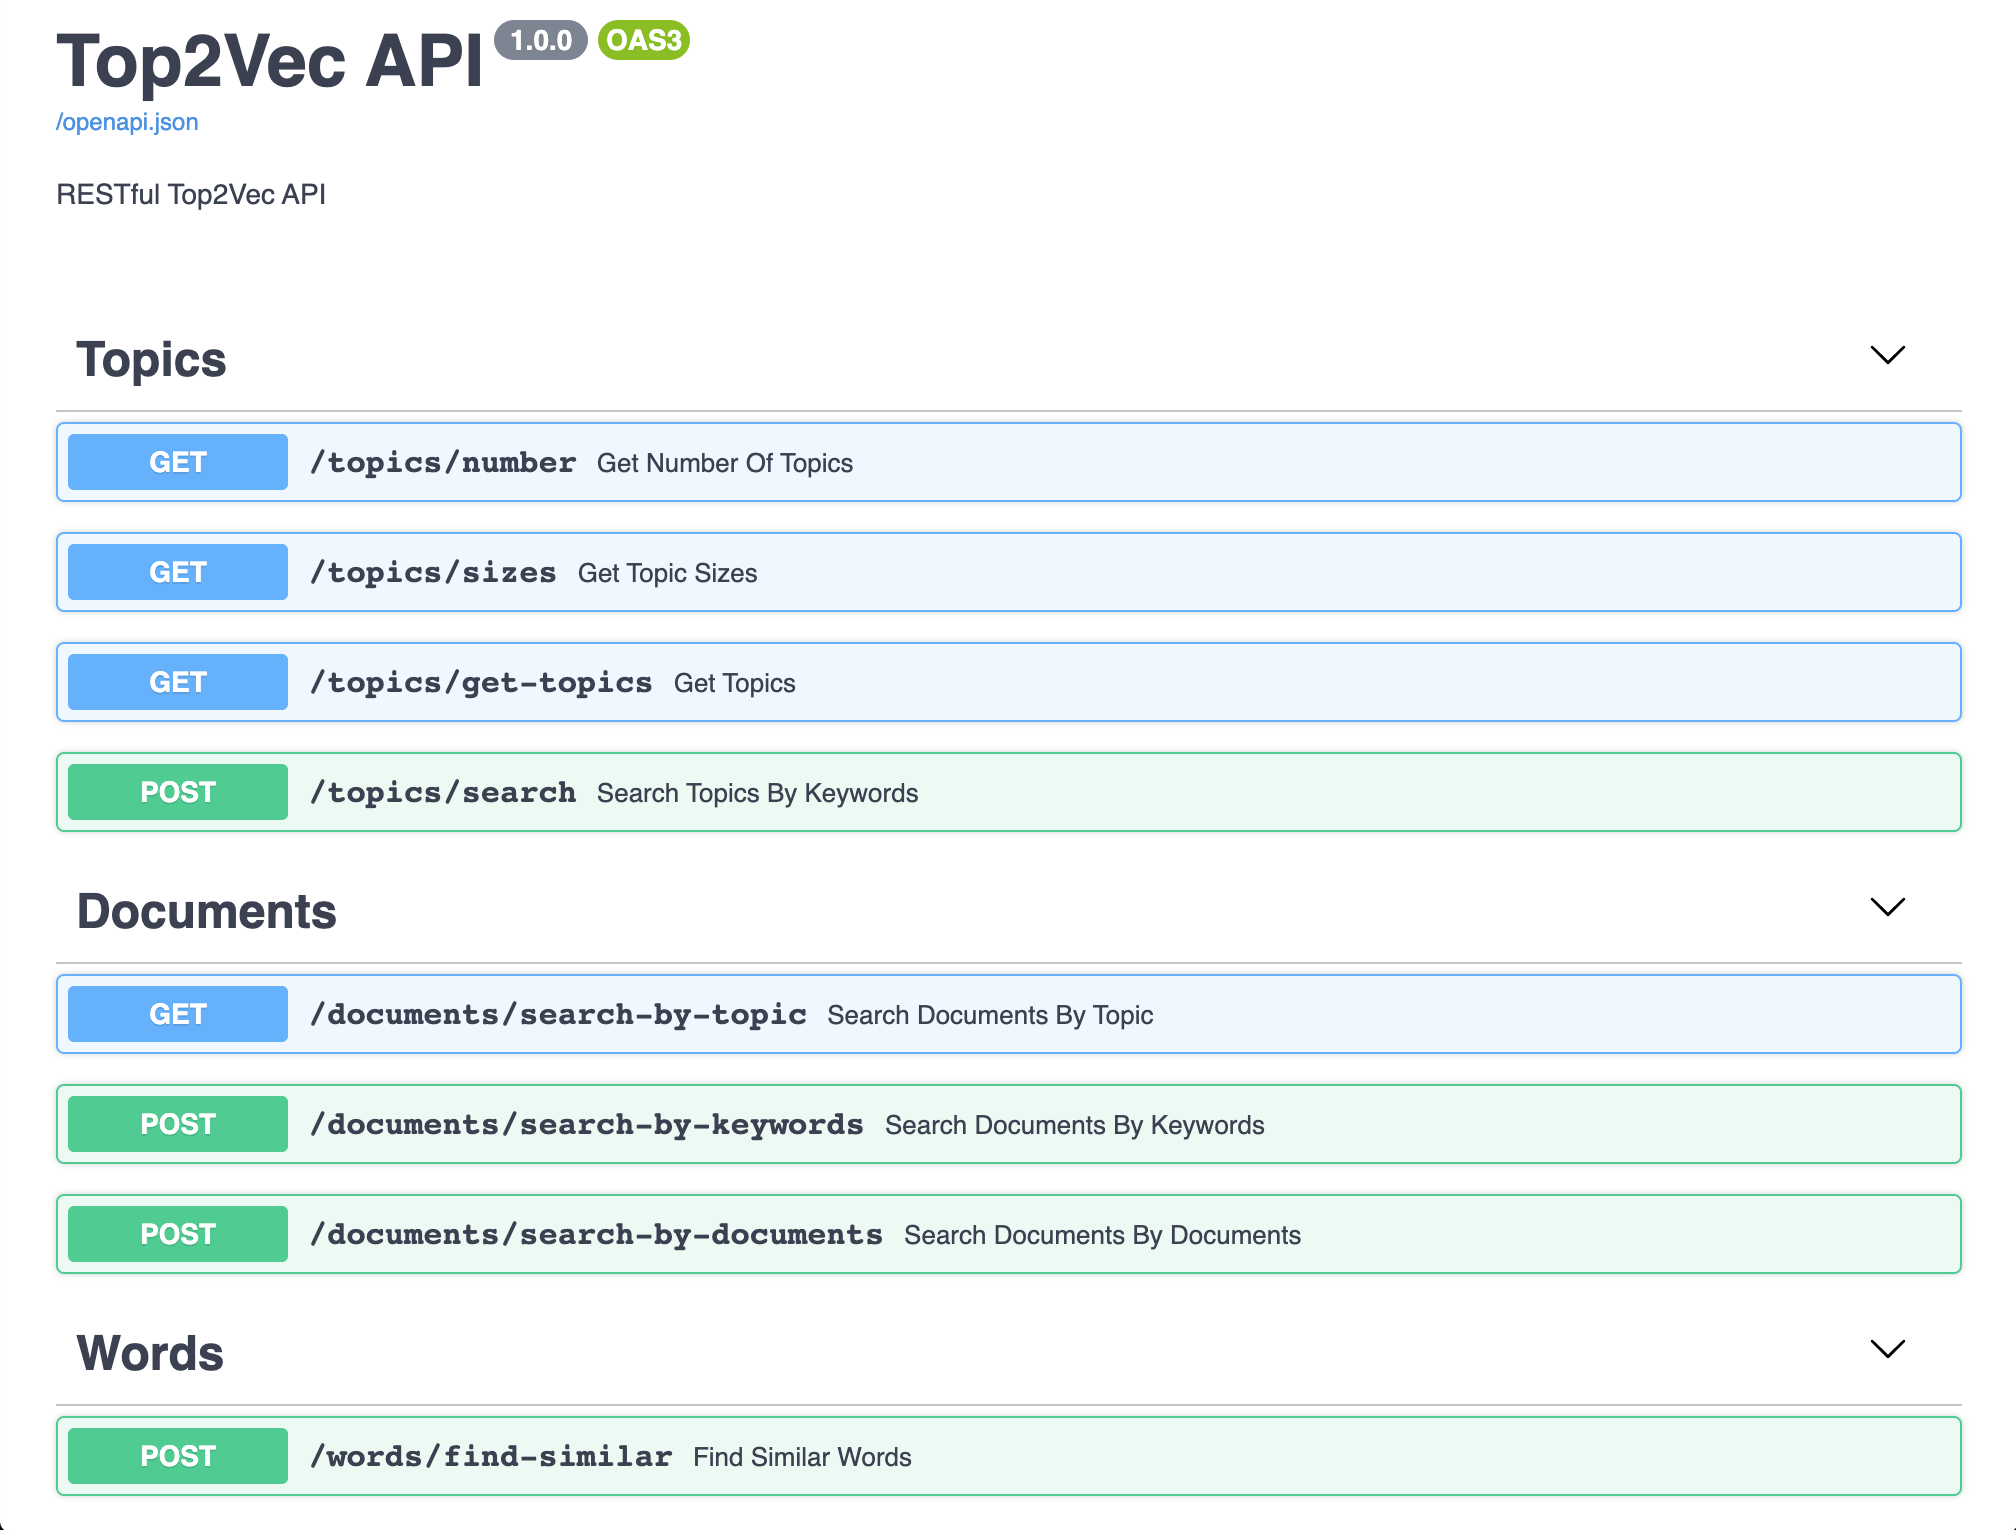
\includegraphics[width=12cm]{img/3.1.restful-top2vec.png}
    \caption{API proposé par Top2Vec}
    \label{fig:api_top2vec}
\end{figure}

\subsubsection{L'algorithme de Top2Vec}
Dans un premier temps, Top2Vec crée des vecteurs de documents et de mots intégrés conjointement à l'aide de Doc2Vec. L'image \ref{fig:docword} illustre un exemple dans lequel les documents qui sont placés à proximité des autres documents similaires et à proximité des mots les plus distinctifs.

\begin{figure}[H] %[!ht]
    \centering
    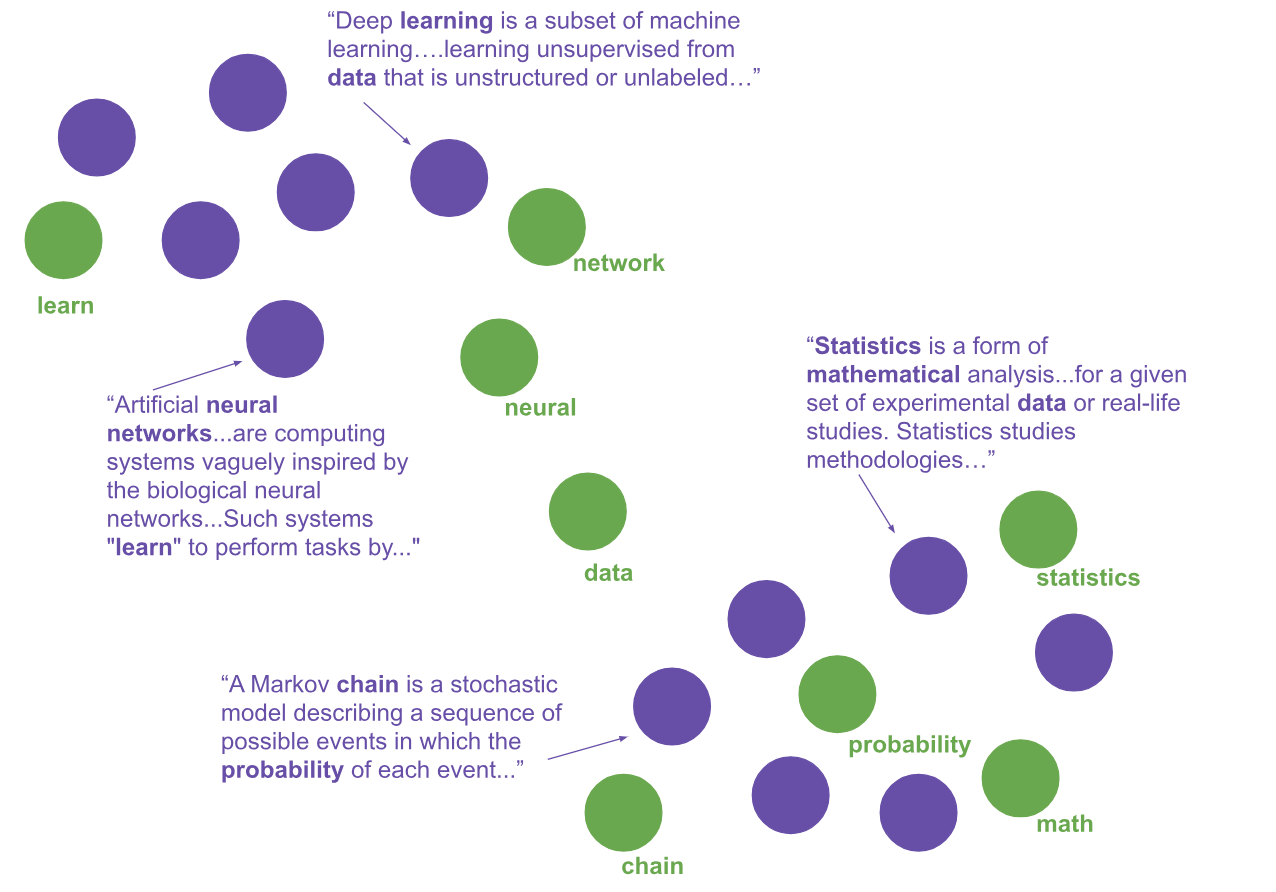
\includegraphics[width=12cm]{img/doc_word_embedding.png}
    \caption{L'emplacement des documents similaires dans l'espace des vecteurs}
    \label{fig:docword}
\end{figure}

Dans le NLP et l’apprentissage automatique, les documents sont souvent représentés sous forme de vecteurs de grande dimension. Chaque dimension de ces vecteurs peut correspondre à un terme (mot) unique dans un vocabulaire, ce qui donne des milliers, voire des millions de dimensions pour un seul document.
Les vecteurs de documents dans un tel espace de grande dimension sont très clairsemés, donc la deuxième étape dans le procès de formation est de réduire des dimensions, qui aide à trouver des zones denses. 
La réduction de dimensions de vecteurs de documents fait référence au processus de réduction des représentations vectorielles originales des documents tout en préservant leurs informations et caractéristiques essentielles.
Cette étape est montrée dans l'image \ref{fig:step2_top2vec}, avec chaque point est un vecteur de document. \footnote{Les images d'illustration de l'algorithme dans cette section sont de la source \cite{Ddangelov}}

\begin{figure}
     \centering
     \begin{subfigure}[b]{0.9\textwidth}
         \centering
         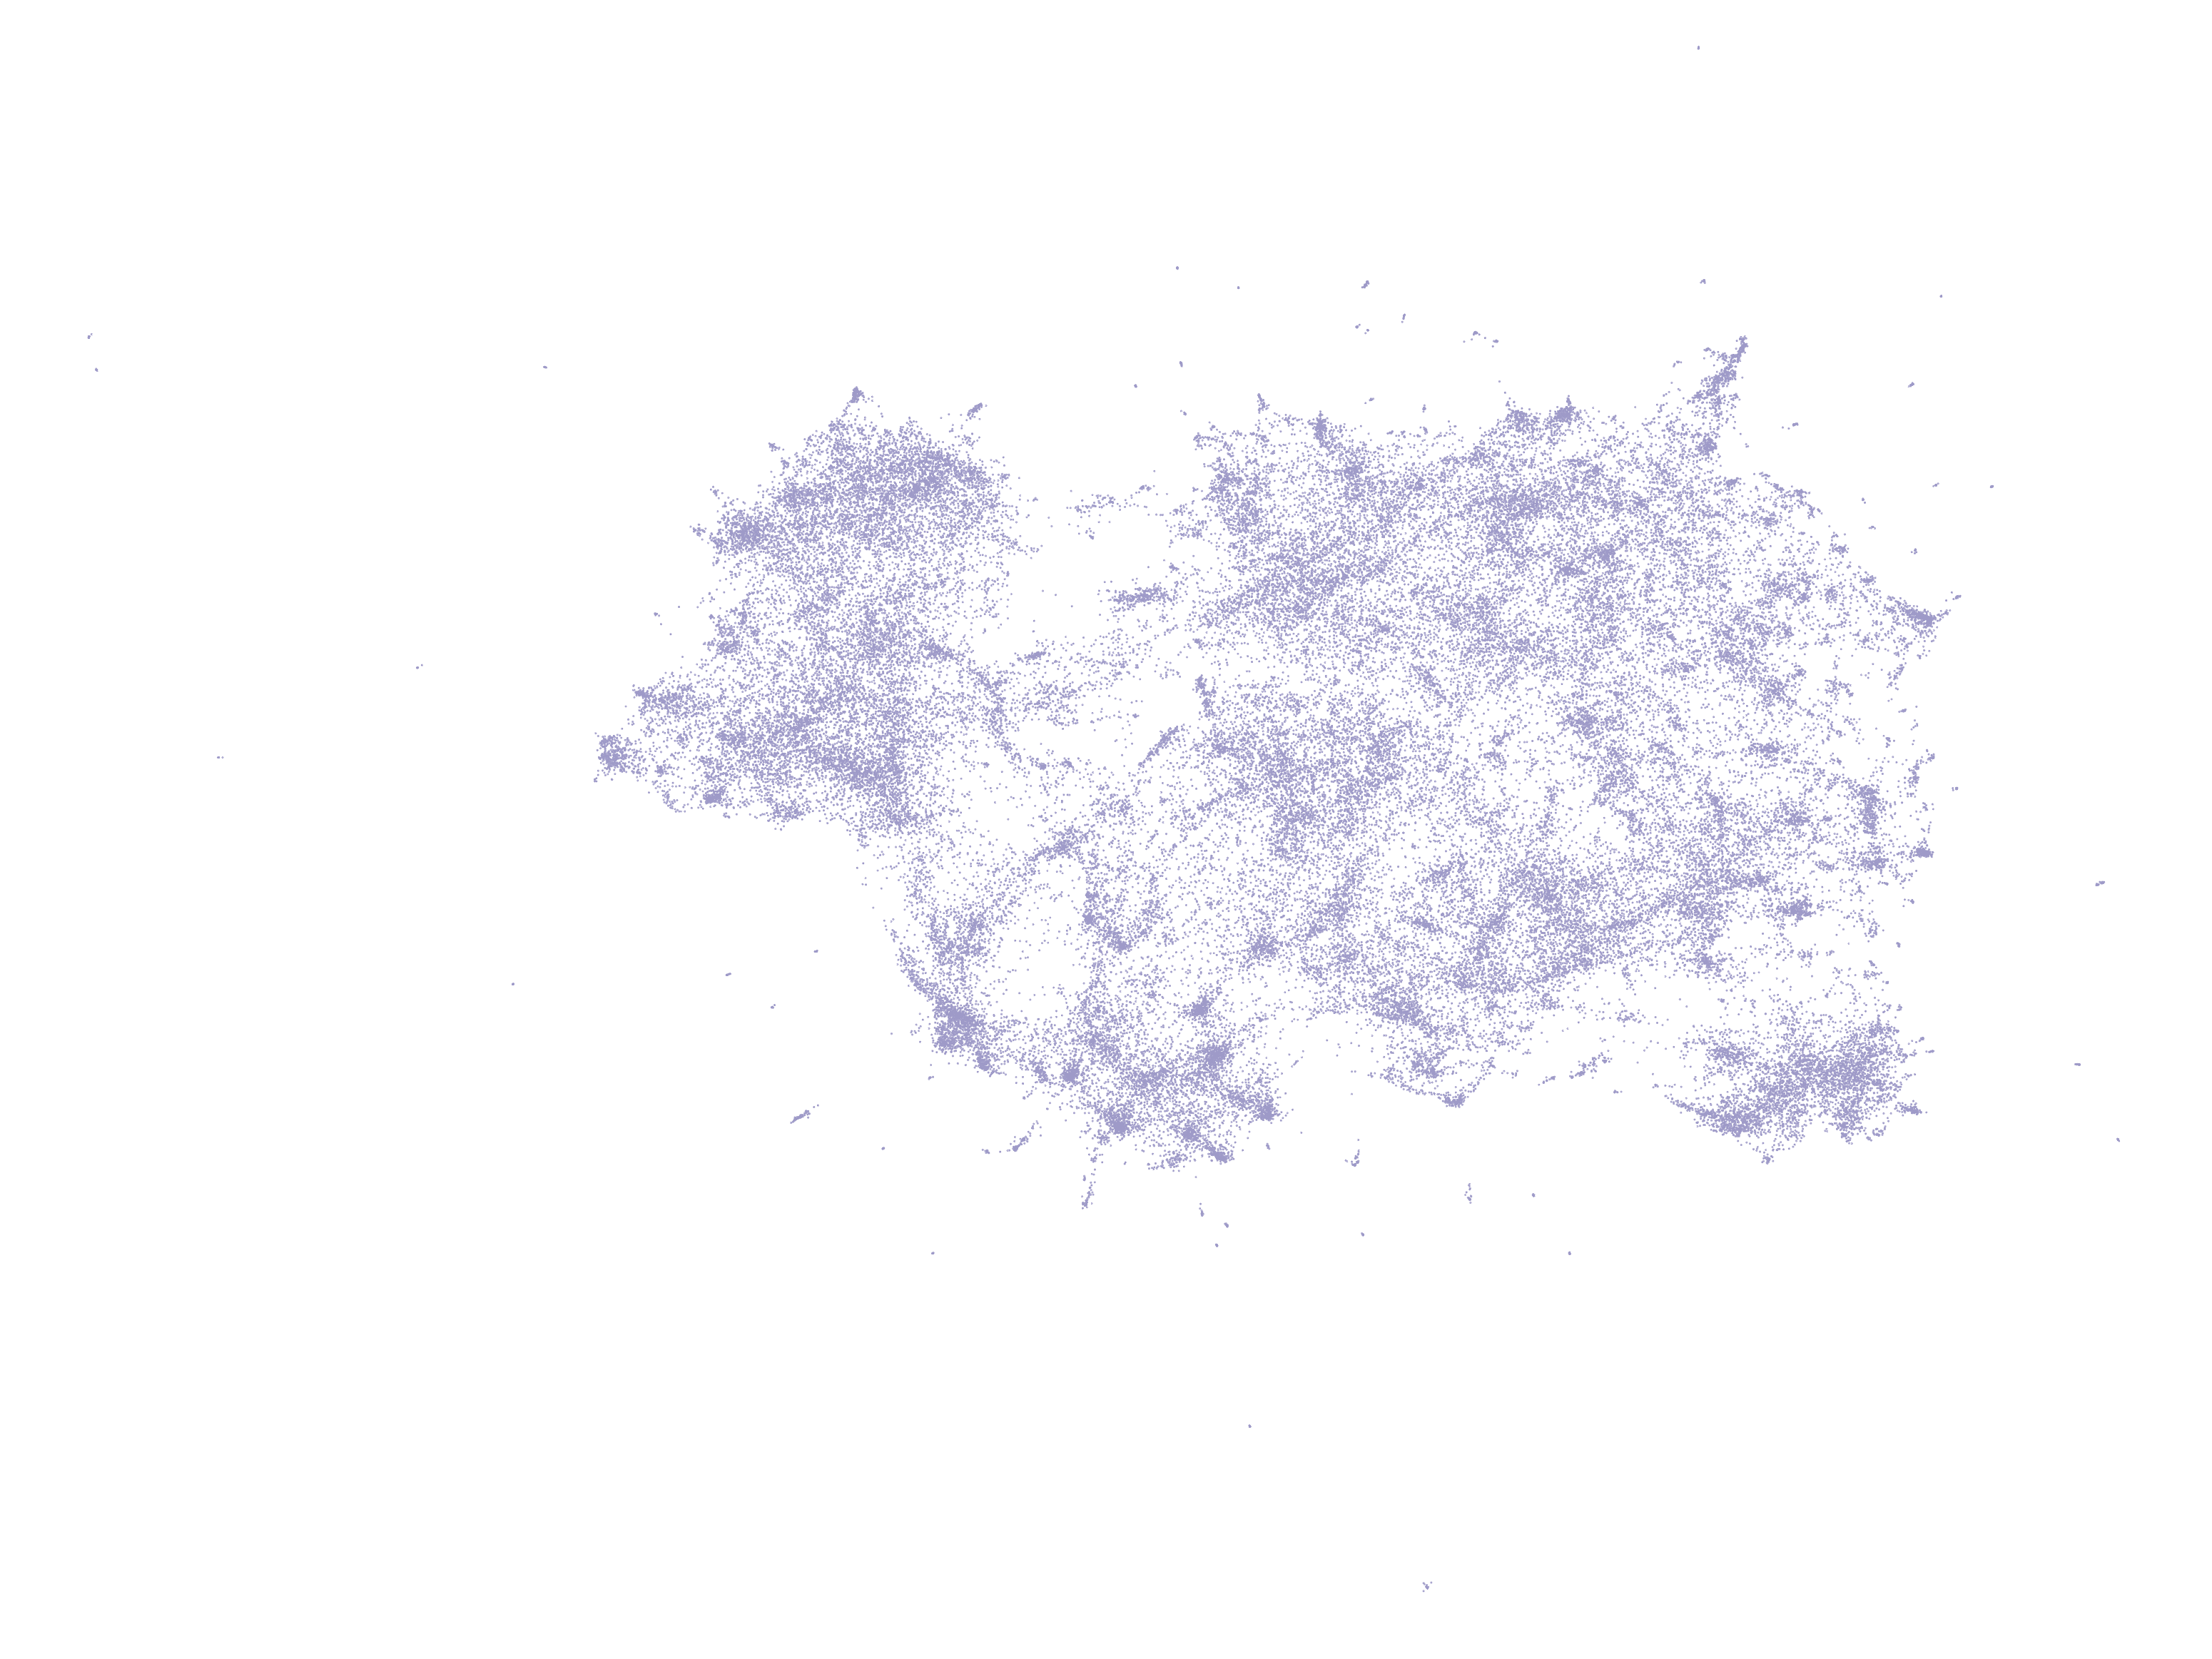
\includegraphics[width=\textwidth]{img/sparse.png}
         \caption{Les vecteurs de grande dimension}
         % \label{fig:tp12_0}
     \end{subfigure}
     \hfill
     \begin{subfigure}[b]{0.9\textwidth}
         \centering
         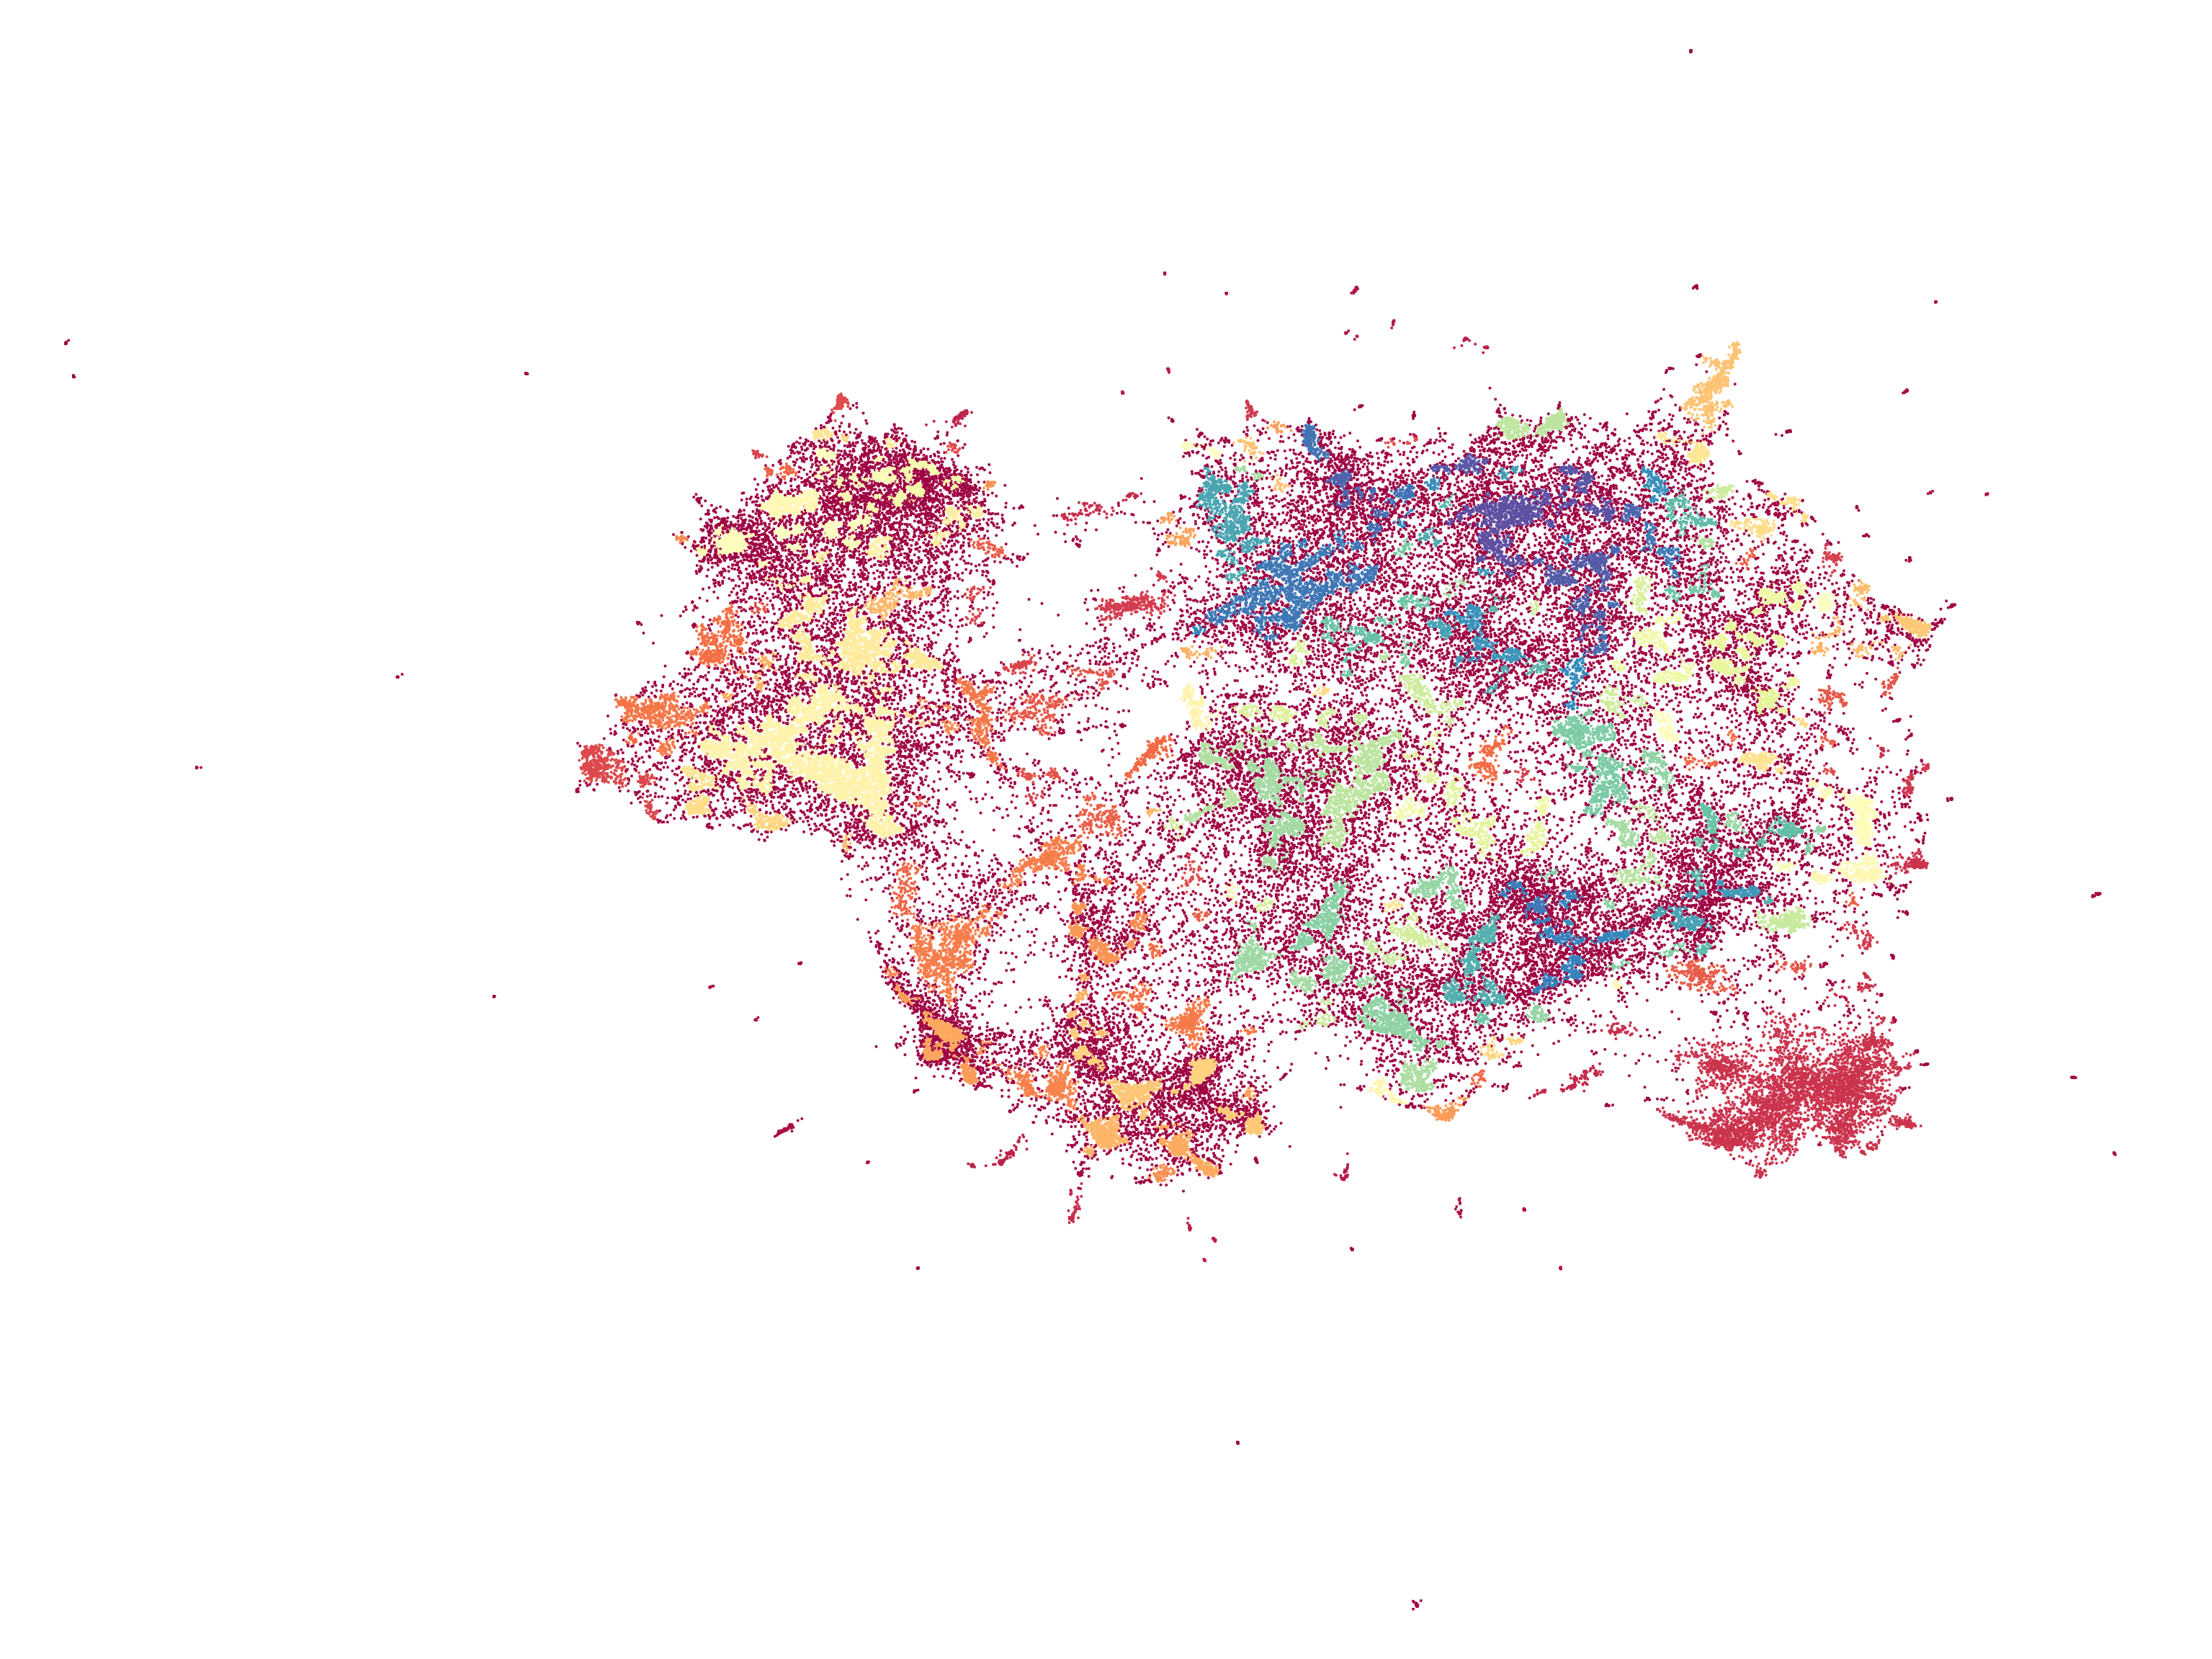
\includegraphics[width=\textwidth]{img/dense.png}
         \caption{Les zones denses des vecteurs de dimension réduite}
         % \label{fig:dense}
     \end{subfigure}
     \hfill
        \caption{La recherche des zones denses avec la réduction de dimension}
    \label{fig:step2_top2vec}
\end{figure}

Ensuite, Top2Vec calcule le centroïde des vecteurs de document pour chaque zone dense, ce centroïde est le vecteur du sujet.
Dans la figure \ref{fig:topic_vector}, les points rouges sont des documents aberrants et ne sont pas utilisés pour calculer le vecteur thématique. Les points violets sont les vecteurs de documents appartenant à une zone dense, à partir de laquelle le vecteur thématique est calculé.

\begin{figure}[H] %[!ht]
    \centering
    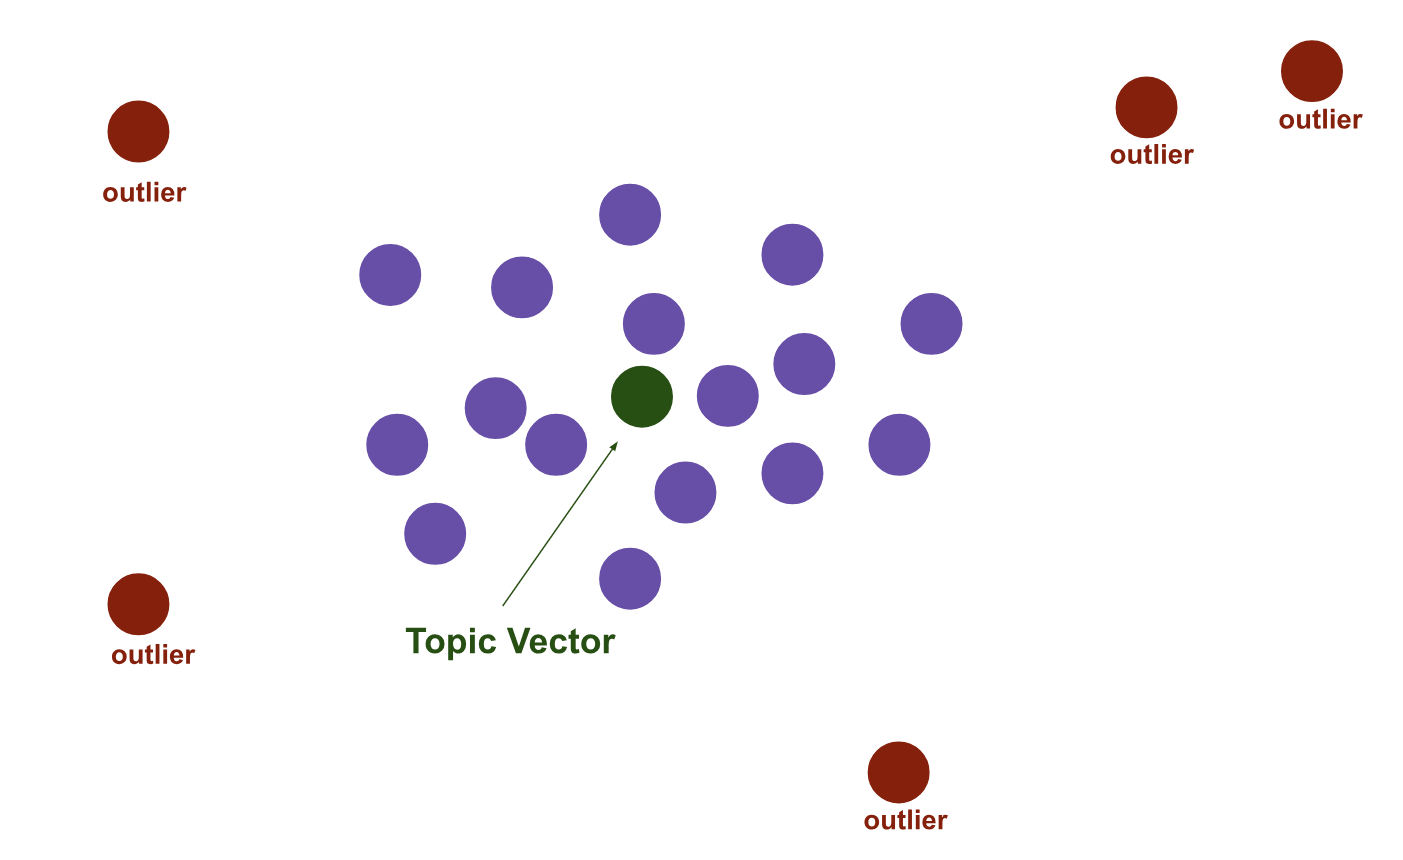
\includegraphics[width=12cm]{img/topic_vector.png}
    \caption{Calcul du centroïde de zone dense alias vecteur du sujet}
    \label{fig:topic_vector}
\end{figure}

Finalement, les vecteurs de mots les plus proches dans la figure \ref{fig:find_keyword} par ordre de proximité deviennent les mots thématiques. Dans Top2Vec, la recherche des plus proches voisins (N-Nearest) est utilisée pour trouver les mots-clés du sujet. 

\begin{figure}[H] %[!ht]
    \centering
    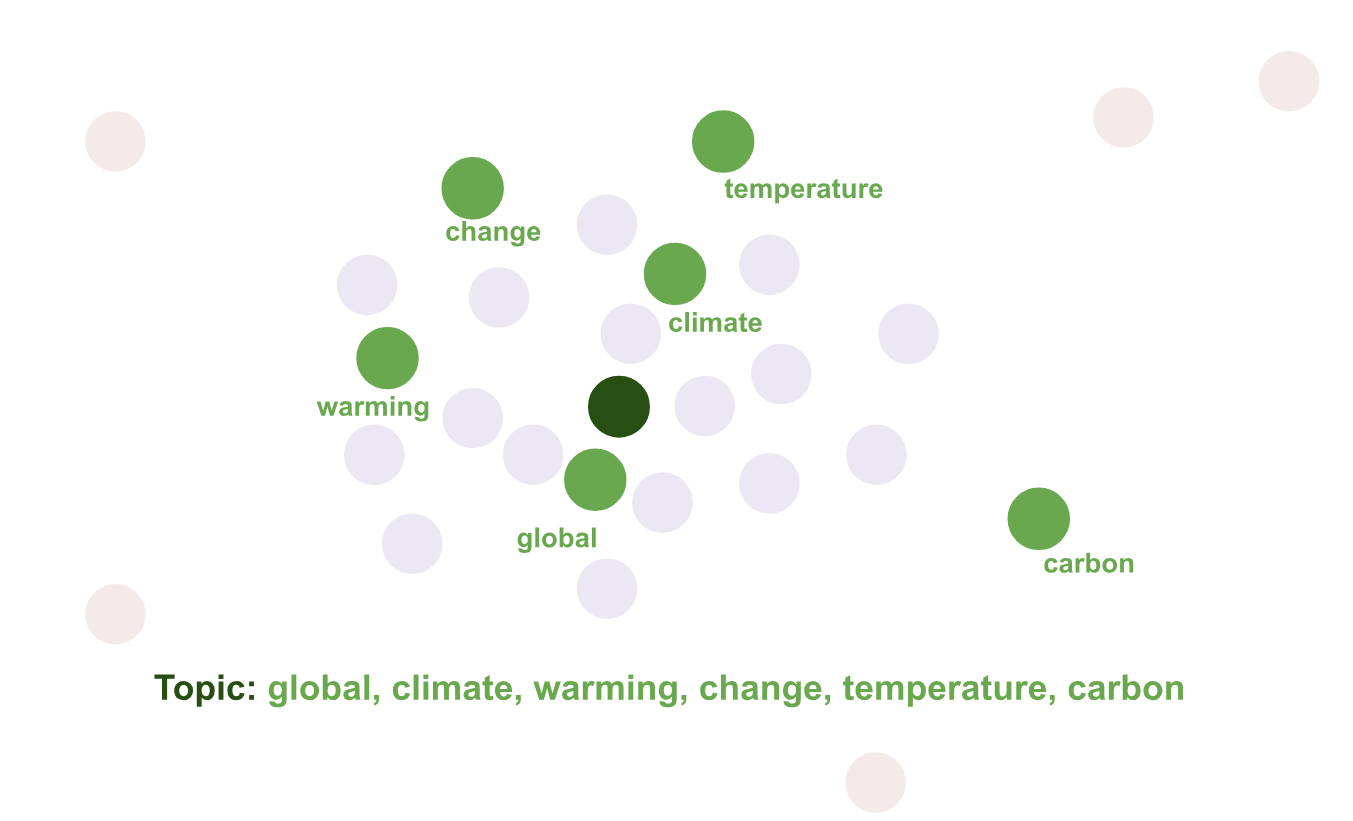
\includegraphics[width=12cm]{img/find_keyword.png}
    \caption{Recherche de mots clés qui sont les mots plus proches au centroïde}
    \label{fig:find_keyword}
\end{figure}

\subsubsection{Structure de l'implémentation}
\textbf{L'objectif de cette étude} est d'effectuer une classification optimale des thèmes présents dans le corpus, en mettant particulièrement l'accent sur les documents de recherche et scientifiques de l'époque de l'Indochine.

Dans la première phase, nous procéderons à plusieurs entraînements en utilisant les modèles LDA et Top2Vec. L'objectif est de comparer l'efficacité de ces deux méthodes. Les résultats devraient confirmer la supériorité de Top2Vec sur LDA en ce qui concerne la modélisation thématique de notre corpus. Nous examinerons également l'impact de certains paramètres essentiels du modèle, notamment le paramètre \textit{min\_count}, qui détermine la fréquence minimale requise pour qu'un mot soit pris en considération, et le paramètre \textit{ngram\_vocab}, qui permet de choisir entre l'analyse de mots individuels ou de collocations n-grammes dans le corpus.

Dans la deuxième phase, nous entreprendrons des ajustements sur le corpus en réduisant certaines catégories de documents moins pertinentes et moins contributives à la thématique scientifique que nous souhaitons identifier. Les résultats de cette étape confirment notre hypothèse selon laquelle le modèle Top2Vec présente encore certaines limites, car il ne parvient pas à détecter les sous-thèmes latents au sein des grands thèmes.

En utilisant un modèle Word2Vec, nous introduisons une étape supplémentaire dans notre processus de modélisation thématique pour les sous-thèmes latents. Nous utilisons des ensembles de mots-clés générés par un modèle Word2Vec bien entraîné, qui prend en compte les mots de faible fréquence dans les documents. Parallèlement, un nouveau modèle Top2Vec est également entraîné en utilisant la même fréquence d'occurrence. Cette approche nous permet d'obtenir des modèles plus compétents dans la compréhension des mots, ce qui facilite la détection précise de petits sous-thèmes associés à des mots-clés spécifiques.

\subsection{Une comparaison de modélisation des sujets entre LDA et Top2Vec}
\subsubsection{LDA performance}
Pour effectuer une allocation de Dirichlet latente (LDA) sur notre corpus, nous utilisons la bibliothèque Gensim. Dans le code ci-dessous, nous créons un dictionnaire Gensim et une représentation de corpus en sac de mots (BoW) à partir du texte prétraité. Ensuite, nous construisons un modèle LDA avec num\_topics = 5 qui définit le nombre de sujets à étudier arbitrairement.

\begin{lstlisting}
# Create a dictionary and a corpus from the preprocessed text
dictionary = corpora.Dictionary(filtered_corpus)
corpus_bow = [dictionary.doc2bow(doc) for doc in filtered_corpus]
# Build the LDA model
lda_model = LdaModel(corpus_bow, num_topics=5, id2word=dictionary, passes=15)
\end{lstlisting}

A la fin de la formation, nous obtenons 5 sujets avec les mots-clés suivants :\newline
\textit{Topic 0: faire,grand,bien,roi,pays,jour,travail,français,cochinchine,chinois \newline
Topic 1: vietnamien,nam,chinois,nguy,langue,étude,thi,bien,histoire,grand\newline
Topic 2: grand,faire,bien,homme,jour,nom,petit,année,chinois,long\newline
Topic 3: société,membre,comité,président,séance,général,saigon,bulletin,etude,secrétaire\newline
Topic 4: saigon,faire,annamite,cochinchine,amiral,lettre,france,pari,bien,français}

Dès la première impression, il est difficile de tirer le thème de chaque sujet en regardant ces mots-clés. Nous essaierons d'extraire quelques documents qui présentent une meilleure similitude dans chaque sujet. Par exemple dans le sujet 0, nous avons trouvé une classe de documents autour du thème de l'architecture ou des monuments de l'époque :\newline
\textit{Document 2 (1799 mots) - Similarité : 1.00 - vue ensemble sculpture modelage chine durant vingt siècles\newline
  Document 3 (11273 mots) - Similarité : 1.00 - vérification dates inscriptions monuments khmers seconde partie\newline
  Document 5 (1501 mots) - Similarité : 0.94 - etude monuments représentatifs art français saigon\newline
}

Mais aussi des documents des chansons :\newline
  \textit{Document 70 (16501 mots) - Similarité : 1.00 - chants antiques montagne\newline
  Document 71 (469 mots) - Similarité : 0.97 - chants populaires proverbes annamites\newline
  Document 114 (1966 mots) - Similarité : 0.98 - folklore musical jara bahnar}

Et les trois grand traductions du roman Les Trois Royaumes qui est le premier des Quatre livres extraordinaires de la littérature classique chinoise :\newline
\textit{Document 190 (73211 mots) - Similarité : 1.00 - trois royaumes traduction notes commentaires nghiêm to louis ricaud\newline
  Document 191 (32268 mots) - Similarité : 1.00 - trois royaumes traduction notes commentaires nghiêm to louis ricaud\newline
  Document 192 (66806 mots) - Similarité : 1.00 - trois royaumes traduction notes commentaires nghiêm to louis ricaud}

Nous constatons une incohérence entre les sujets des documents, qui s'explique principalement par le fait que la méthode LDA est basée sur un ensemble de mots fréquemment associés à ce sujet et pas sur leur relation thématique. LDA nécessite la spécification de paramètres, tels que le nombre de sujets (num\_topics). Si ces paramètres ne sont pas choisis de manière appropriée pour le corpus, les sujets résultants risquent de ne pas être significatifs. Le réglage de ces paramètres peut être difficile et nécessite souvent une expertise du domaine.
Dans ce travail, plusieurs tentatives sur différents paramètres ont été faites mais aucune ne propose une modélisation significative.
\footnote{Les résultats de deux autres modèles de 12 sujets et 24 sujets sont inclus en annexe de cette memoire.}

\subsubsection{Top2Vec performance}
La formation du Top2Vec est implémentée comme suit :
\begin{lstlisting}
from top2vec import Top2Vec
import multiprocessing
# Initialize Top2Vec model
model_T2V = Top2Vec(documents=preprocessed_corpus, 
                tokenizer=lambda x: x.split(), 
                min_count=200,
                speed='deep-learn',
                workers=(multiprocessing.cpu_count())
               )
\end{lstlisting}
Dans cet appel, le paramètre 'min\_count' représente la fréquence minimale à laquelle chaque mot doit apparaître dans le corpus pour être pris en compte. Par exemple, min\_count=100 exige que chaque mot soit présent au moins 100 fois dans le corpus pour être inclus dans le modèle. Le paramètre 'speed' détermine la vitesse à laquelle le modèle est entraîné. L'option 'fast-learn' est la plus rapide mais génère des vecteurs de moindre qualité. L'option 'learn' génère des vecteurs de meilleure qualité mais prend plus de temps à s'entraîner. L'option 'deep-learn' apprend les vecteurs de la meilleure qualité mais nécessite beaucoup plus de temps d'entraînement. Comme l'option 'deep-learn' est choisie, le nombre maximal de threads de travail (workers) est utilisé pour accélérer la formation du modèle.

Nous présentons ici un modèle entraîné avec les mots apparaissant au moins 200 fois. Après l'apprentissage automatique, Top2Vec retourne un regroupement de 10 sujets avec les mots-clés suivants :

\begin{tabular}{|p{15cm}|}
\hline
Regroupement des sujets et les mot-clés\\
\hline
\textbf{Sujet} \textbf{1 }:  lecteur,  pensée,  savant,  étudier,  historien,  civilisation  scientifique,  intellectuel,  auteur,  ouvrage \\ \hline
\textbf{Sujet} \textbf{2} :  surface,  liquide,  sec,  couche,  mètre,  diamètre,  épaisseur,  sol , profondeur,  tige\\ \hline
\textbf{Sujet} \textbf{3} : comité,  membre,  bulletin,  secrétaire,  président,  séance,  réunion  assemblée,  publication,  commission \\ \hline
\textbf{Sujet} \textbf{4} :  amiral,  navire,  capitaine,  expédition,  commandant,  marine  gouvernement,  armer,  établissement,  port \\ \hline
\textbf{Sujet} \textbf{5} : génie,  offrande,  prière,  buffle,  divinité,  parent,  autel  laotien,  maison,  sacrifice \\ \hline
\textbf{Sujet} \textbf{6} :  monument,  angkor,  relief,  sculpture,  édifice,  temple,  style  statue,  khmèr,  décor \\ \hline
\textbf{Sujet} \textbf{7} :  nên,  làm,  nào,  qua,  cœur,  cho,  khi,  mari,  aimer,  nhà  \\ \hline
\textbf{Sujet} \textbf{8} :  asia,  studie,  vietnam,  asie,  rét,  thai,  tnam,  viet,  van,  nam \\ \hline
\textbf{Sujet} \textbf{9} :  géographie,  agriculture,  société,  annal,  journal,  revue,  agricole  colonial,  indo,  tonkin \\ \hline
\textbf{Sujet} \textbf{10} :  directeur,  professeur,  secrétaire,  rue,  président,  administrateur  général,  collège,  colonial,  municipal \\ 
\hline
\end{tabular}
\vspace{1cm}

Intuitivement, les mots-clés de chaque sujet se présentent de manière plus cohérente autour d'un thème spécifique, ce qui nous permet de nommer directement chaque sujet. Par exemple, le thème 1 couvre des mots liés à l'agriculture et aux plantations, le thème 3 s'agit des documents militaires, et le thème 5 mentionne l'architecture et les monuments d'Angkor-Vat (Cambodge). Voici une liste de documents faisant partie des documents les plus similaires dans le sujet "Agriculture" :
\begin{itemize}
    \item culture de l \textbf{abaca} lettre de m le gérant du consulat général de manille 1889
    \item courtes notices sur l indochine i l opium ii les \textbf{pêcheries} la \textbf{préparation} du nuoc mam les salines 1898
    \item rapport présenté par m j josselme sur la culture du \textbf{rocou} 1883 
    \item rapport sur la culture du \textbf{jute} 1895 
    \item de la préparation en cochinchine des \textbf{fromages} de pate de \textbf{haricots} \item notice sur la culture du \textbf{café} libéria 1888
    \item remarques faites dans le drainage d une \textbf{tourbière bois} de trams et armes ou outils en pierre taillée dans la \textbf{tourbe} 1884 
    \item mémoire sur le \textbf{sulfatage} des \textbf{céréales} 1883
    \item notice sur le mac lua \textbf{plante} \textbf{tinctoriale} 1887 
\end{itemize}


On peut observer dans la figure \ref{fig:heatmap} les cartes thermiques (heatmap) qui visualisent les scores de similarité entre 4 modèles en faisant varier les valeurs de min\_count entre 50, 100, 200 et 400. De manière générale, on constate une faible similarité entre les différents sujets. Le modèle avec une fréquence d'occurrence des mots comprise entre 100 et 200 génère plus de sujets que les modèles avec un min\_count de 50 ou 400, ce qui confirme notre hypothèse selon laquelle il existe une plage de fréquence à laquelle les mots deviennent plus bruyants (faible/moyenne fréquence, par exemple 50) ou plus génériques (haute fréquence, par exemple 400). En ce qui concerne la similarité, le modèle à 100 fréquences présente les meilleurs résultats, car il comporte moins de sujets fortement similaires que le modèle à 200 fréquences, par exemple les sujets 7, 8 et 9.

\begin{figure}[H]
        \centering
        \begin{subfigure}[b]{0.45\textwidth}
            \centering
            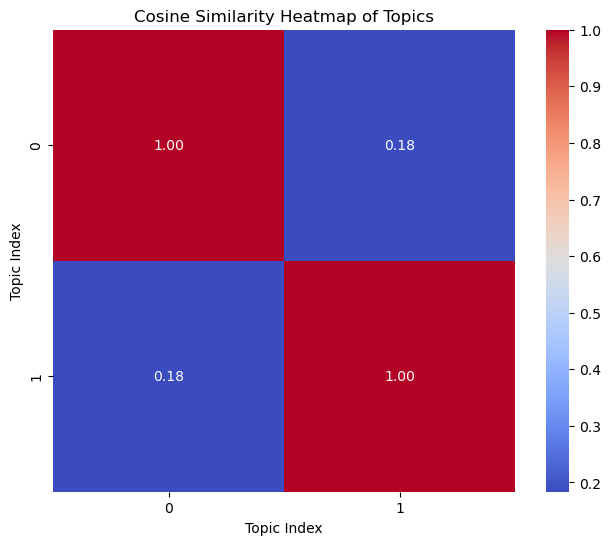
\includegraphics[width=\textwidth]{img/3.2acosine_sim_50_ngram_deep.png}
            \caption[min\_count = 50]%
            {{\small min\_count = 50}}    
            % \label{fig:50}
        \end{subfigure}
        \hfill
        \begin{subfigure}[b]{0.45\textwidth}  
            \centering 
            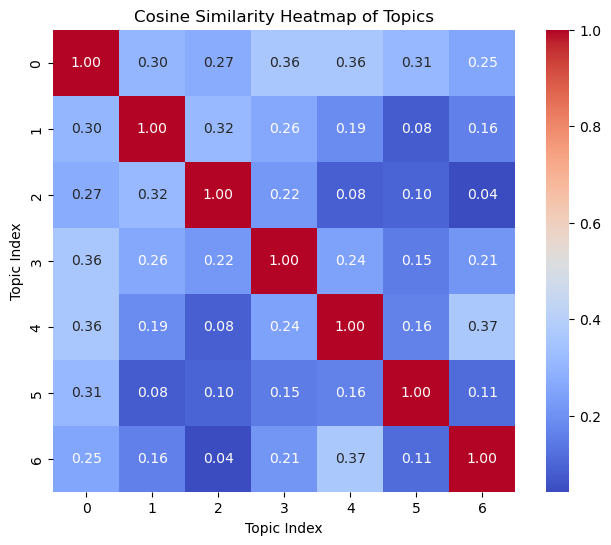
\includegraphics[width=\textwidth]{img/3.2bcosine_sim_100_ngram_deep.png}
            \caption[min\_count = 100]%
            {{\small min\_count = 100}}    
            % \label{fig:100}
        \end{subfigure}
        \vskip\baselineskip
        \begin{subfigure}[b]{0.45\textwidth}   
            \centering 
            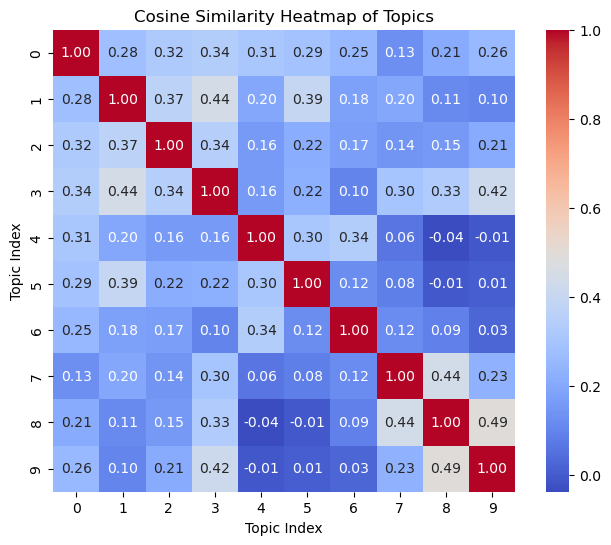
\includegraphics[width=\textwidth]{img/3.2ccosine_sim_200_ngram_deep.png}
            \caption[min\_count = 200]%
            {{\small min\_count = 200}}    
            % \label{fig:200}
        \end{subfigure}
        \hfill
        \begin{subfigure}[b]{0.45\textwidth}   
            \centering 
            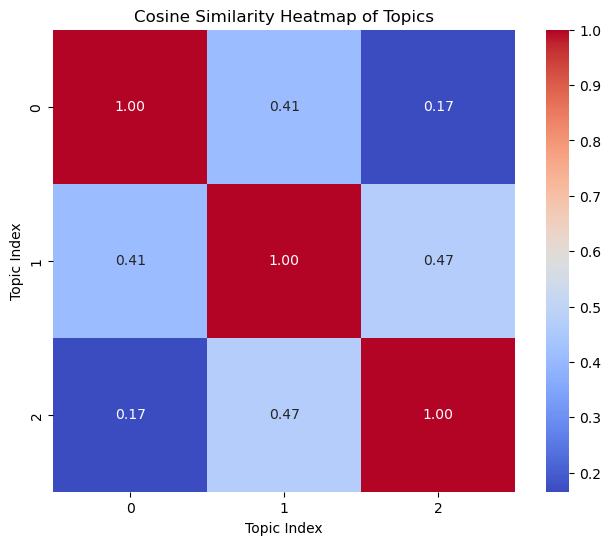
\includegraphics[width=\textwidth]{img/3.2d.cosine_sim_400_ngram_deep.png}
            \caption[min\_count = 400]%
            {{min\_count = 400}}    
            % \label{fig:400}
        \end{subfigure}
        \caption {Carte thermique de la similarité du modèle utilisant différentes valeurs min\_count}
        \label{fig:heatmap}
    \end{figure}

\subsubsection{Entraînement  des sujets avec les collocations ngram}
Non seulement il regroupe les documents en fonction de l'entraînement des mots individuels, mais Top2Vec est également capable de détecter les expressions courantes dans le corpus et de les ajouter au vocabulaire des sujets.

En utilisant le paramètre \textit{ngram\_vocab = True}, le modèle s'entraîne  pour repérer les collocations fréquentes et les considérera lors de la classification des sujets, ce qui renforcera davantage l'identité de chaque sujet par rapport aux mots individuels.

\begin{lstlisting}
mincount = 200
train_speed = 'deep-learn'
model_test_param = Top2Vec(documents=preprocessed_corpus, 
            tokenizer=lambda x: x.split(), 
            min_count=mincount,
                ngram_vocab = True,
            speed=train_speed,
            workers=(multiprocessing.cpu_count() )
           )
model_test_param.save(f'model_ngram_{mincount}_{train_speed}')
\end{lstlisting}

La Figure \ref{wc_militaire_2gram} présente le nuage de mots générés pour le sujet militaire, qui inclut des bigrammes tels que "expédition militaire", "armée canon", "capitaine vaisseau", "port Touraine".

\begin{figure}[H] %[!ht]
    \centering
    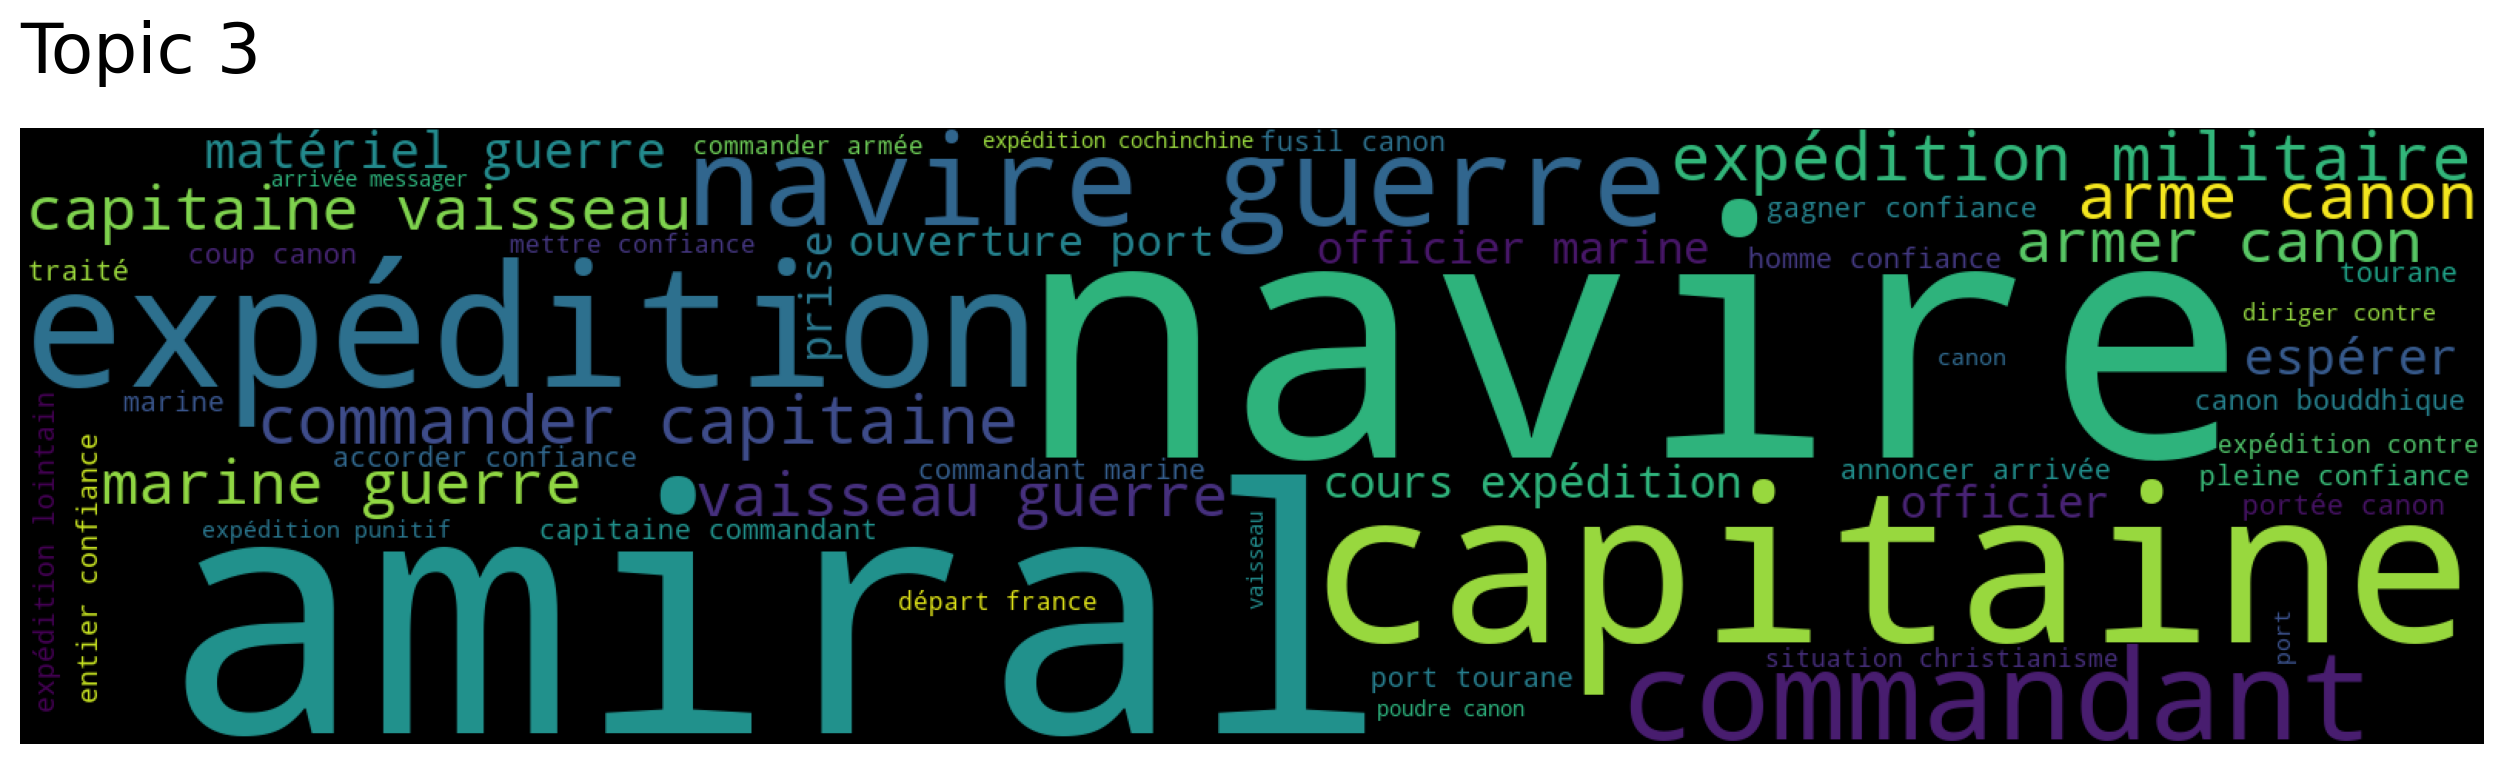
\includegraphics[width=14cm]{img/3.4.wc_militaire.png}
    \caption{WordCloud du sujet militaire avec un modèle de ngram\_vocab}
    \label{wc_militaire_2gram}
\end{figure}

\subsection{Analyses des significations des sujets}

La Figure \ref{fig:topic_size_docs} illustre la distribution de documents parmi les sujets regroupés, y compris ceux que nous avons considérés comme peu utiles, obtenus à la suite d'un entraînement avec l'option ngram\_vocab. Nous pouvons observer que trois grands sujets, à savoir "recherche générale", "militaire" et "traduction/bilingue en vietnamien", représentent une grande partie du corpus, tandis que les groupes de documents 7, 9 et 10 contiennent très peu de documents. Un autre groupe que nous avons identifié  comme "divers" - groupe 4 par contre inclut beaucoup de documents, avec les autres sujets tels que "agriculture", "architecture", "ethnies du Laos", "études asiatiques" et "traduction/bilingue en chinois", chacun de ces sujets occupe également une part importante du corpus. Nous allons examiner de plus près le contenu de chaque groupe de documents afin de mieux comprendre leur vraie signification. Nous espérons identifier les avantages et les inconvénients de cette méthode de regroupement.

\begin{figure}[H] %[!ht]
    \centering
    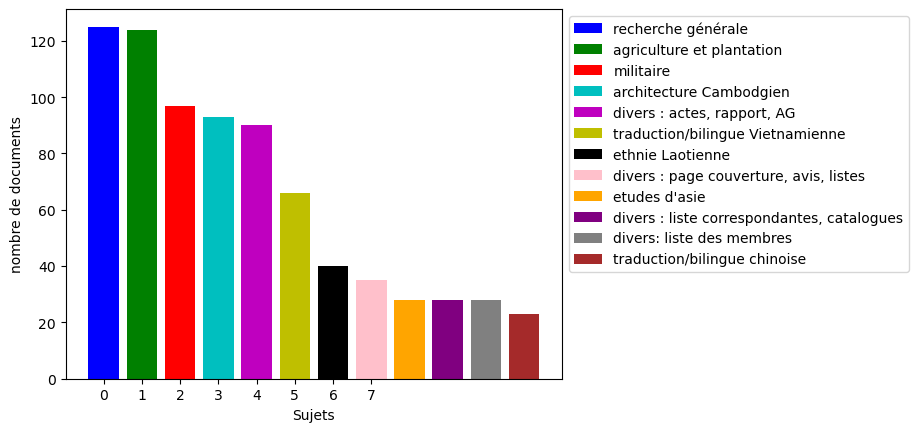
\includegraphics[width=14cm]{img/topic_size_docs.png}
    \caption{Répartition du nombre de documents entre les sujets regroupés}
    \label{fig:topic_size_docs}
\end{figure}

En plus du sujet militaire que nous avons examiné en détail avec son nuage de mots dans la section précédente (voir Figure \ref{wc_militaire_2gram}), notre analyse a également identifié d'autres sujets populaires dans le corpus qui sont détectés de manière assez précise. Parmi ces sujets figurent "Agriculture et Plantation" ainsi que "Recherche générale," qui comprend principalement des documents de recherche en histoire et en sciences humaines. Les nuages de mots correspondants sont visibles dans les Figure \ref{fig:tp12_0} et \ref{fig:tp12_1}.

Cependant, l'inconvénient de ces sujets est qu'ils semblent être un peu trop généraux en ce qui concerne les thèmes qu'ils englobent. Cela suggère qu'il existe encore davantage de sujets intéressants qui se cachent sous chaque thème principal. Par exemple, dans le sujet 1 - "Agriculture et Plantation," il est possible de trouver des articles portant sur des sujets tels que la médecine et les maladies, la nourriture ou la cuisine de l'époque. De même, dans le sujet 0 - "Recherche historique et humanités," les sujets de recherche demeurent trop vastes et peuvent englober d'autres thèmes plus spécifiques à l'intérieur de leur champ d'étude.

\begin{figure}[H]
     \centering
     \begin{subfigure}[b]{0.9\textwidth}
         \centering
         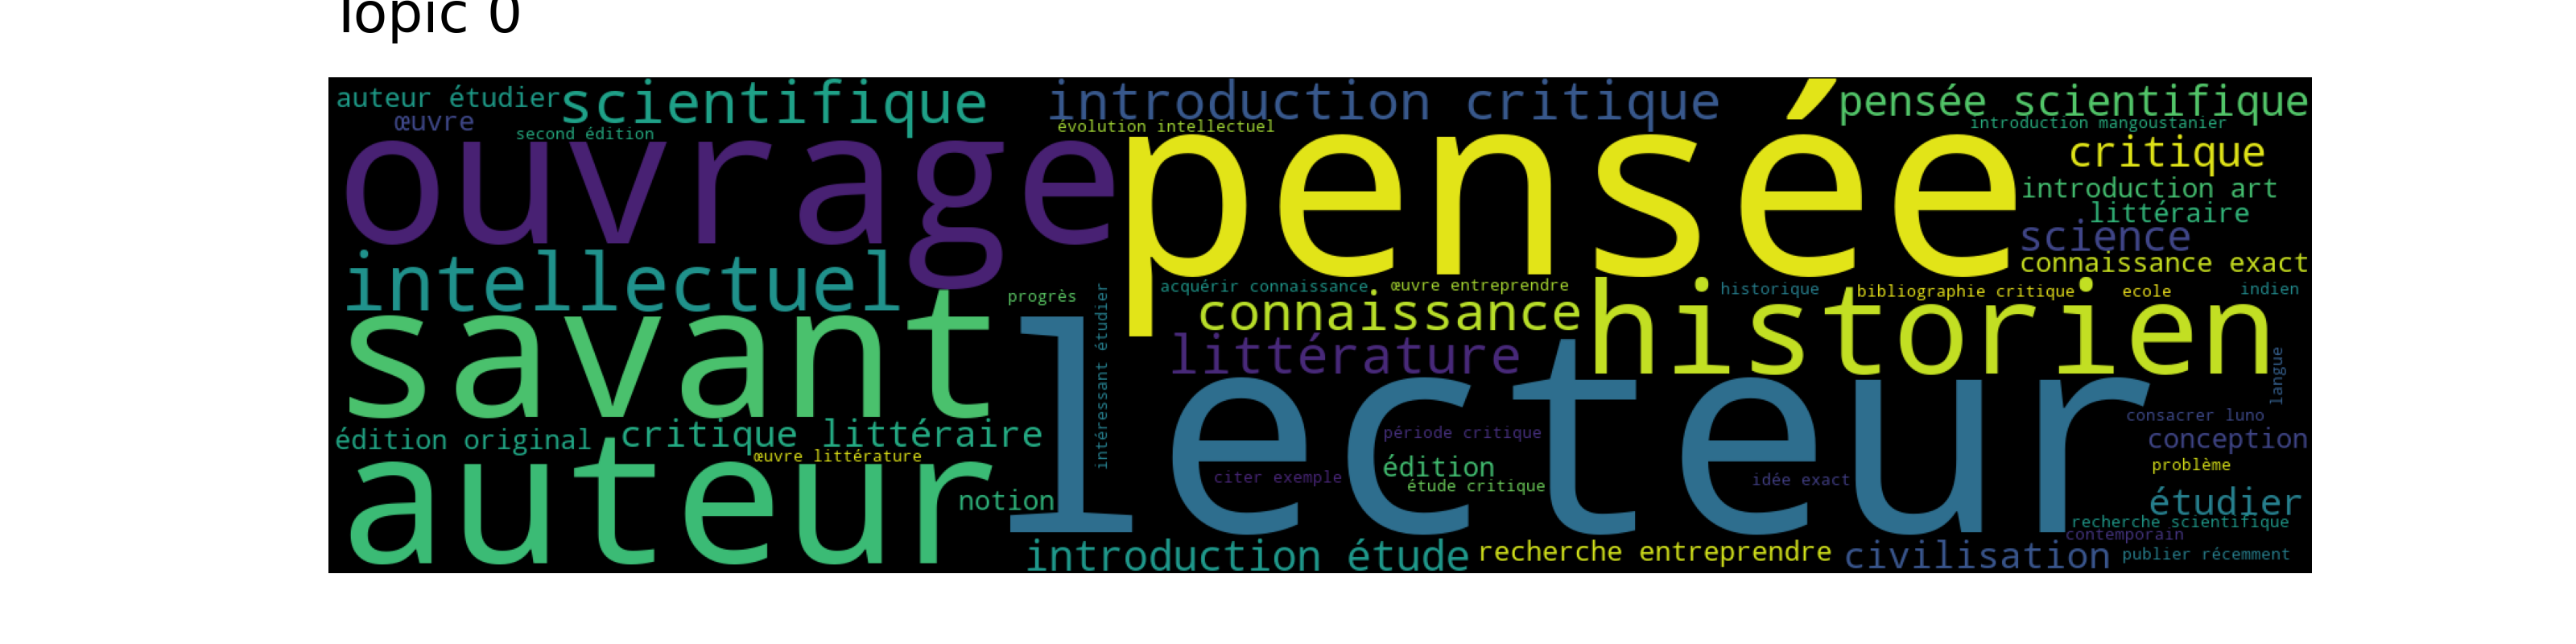
\includegraphics[width=\textwidth]{img/wordcloud model ngram 200 topic 0 .png}
         \caption{Recherche historique et humanité}
         \label{fig:tp12_0}
     \end{subfigure}
     \hfill
     \begin{subfigure}[b]{0.9\textwidth}
         \centering
         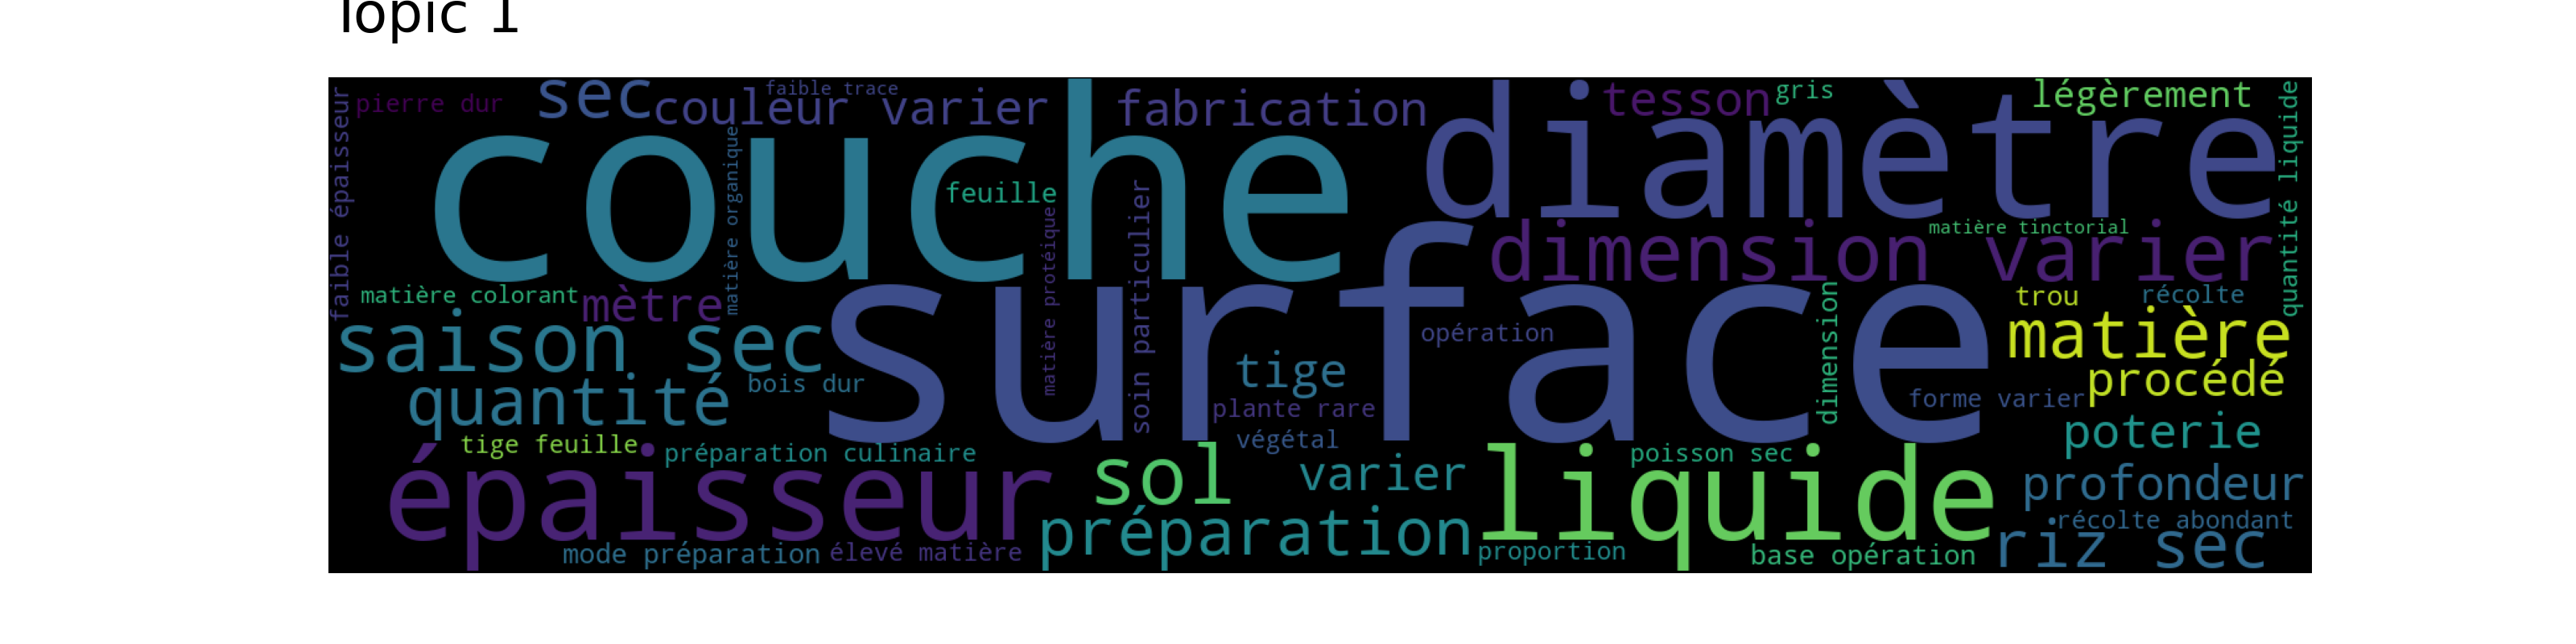
\includegraphics[width=\textwidth]{img/wordcloud model ngram 200 topic 1 .png}
         \caption{Agriculture et Plantation}
         \label{fig:tp12_1}
     \end{subfigure}
     \hfill
        \caption{Les grands sujets du corpus}
    % \label{fig:2_big_topic}
\end{figure}

En outre, certains sujets sont très bien regroupés avec une belle cohérence de contenu dans les documents. La Figure \ref{fig:lao_cam} illustre les nuages de mots pour les sujets "Culture et Architecture Khmer Cambodgien" et "Les ethnies Vietnamiennes/Laotiennes".

\begin{figure}[ht]
     \centering
     \begin{subfigure}[b]{0.9\textwidth}
         \centering
         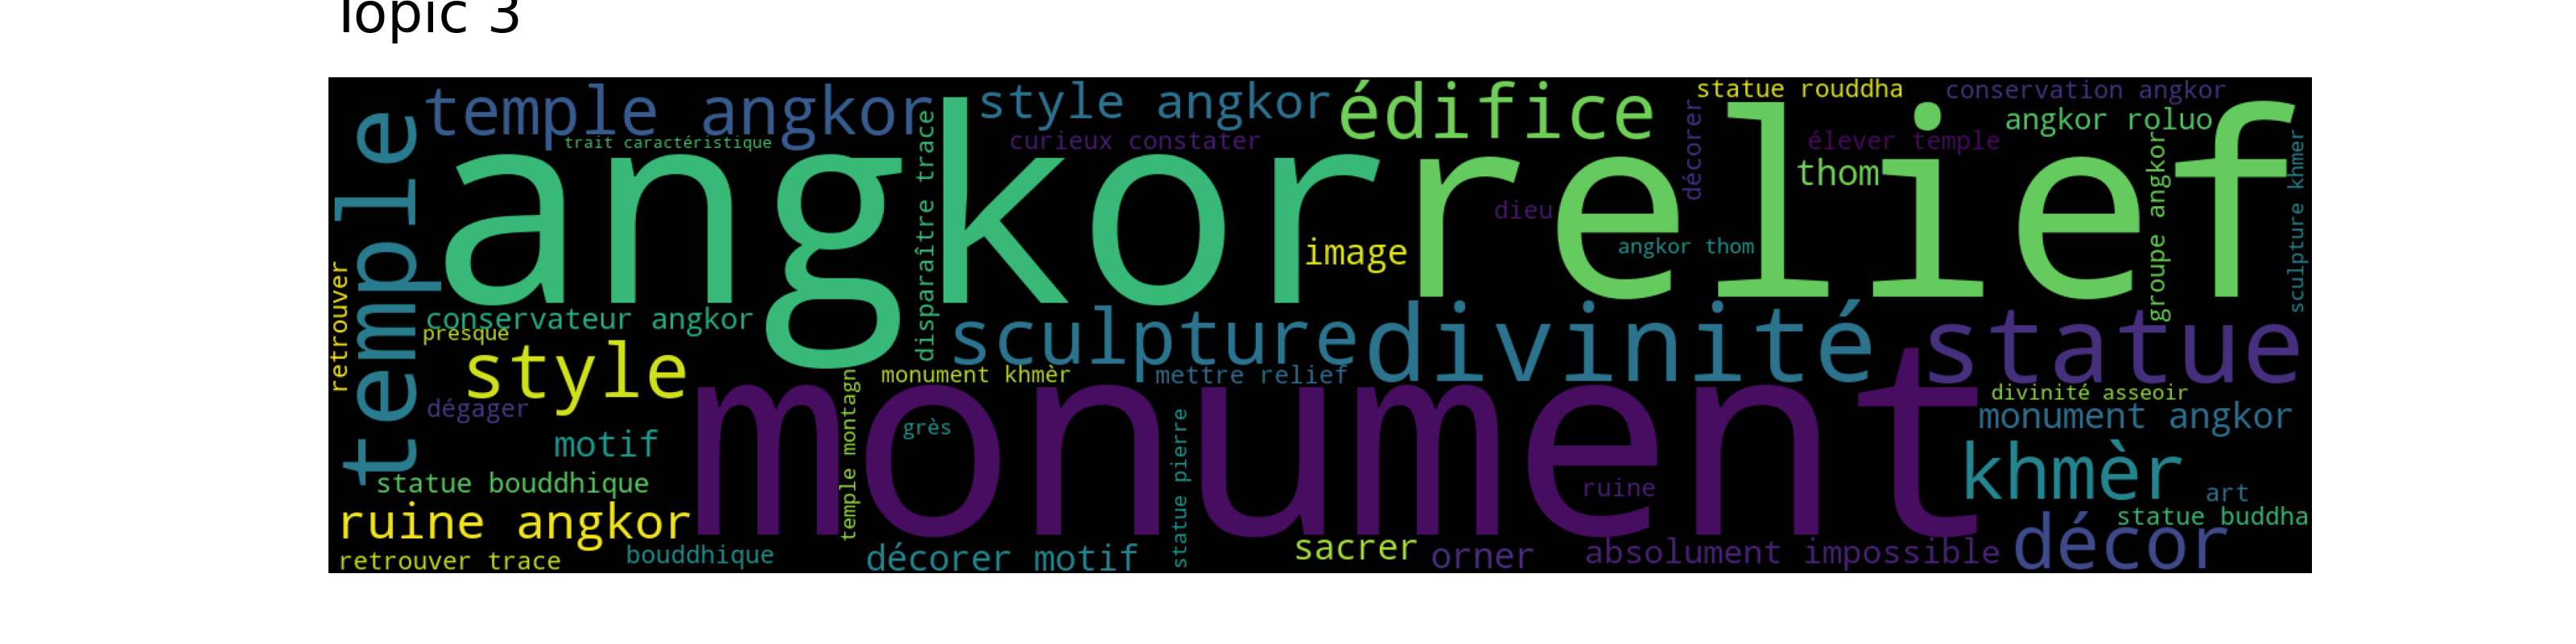
\includegraphics[width=\textwidth]{img/wordcloud model ngram 200 topic 3 .png}
         \caption{Culture et Architecture Khmer Cambodgien}
         \label{fig:tp12_3}
     \end{subfigure}
     \hfill
     \begin{subfigure}[b]{0.9\textwidth}
         \centering
         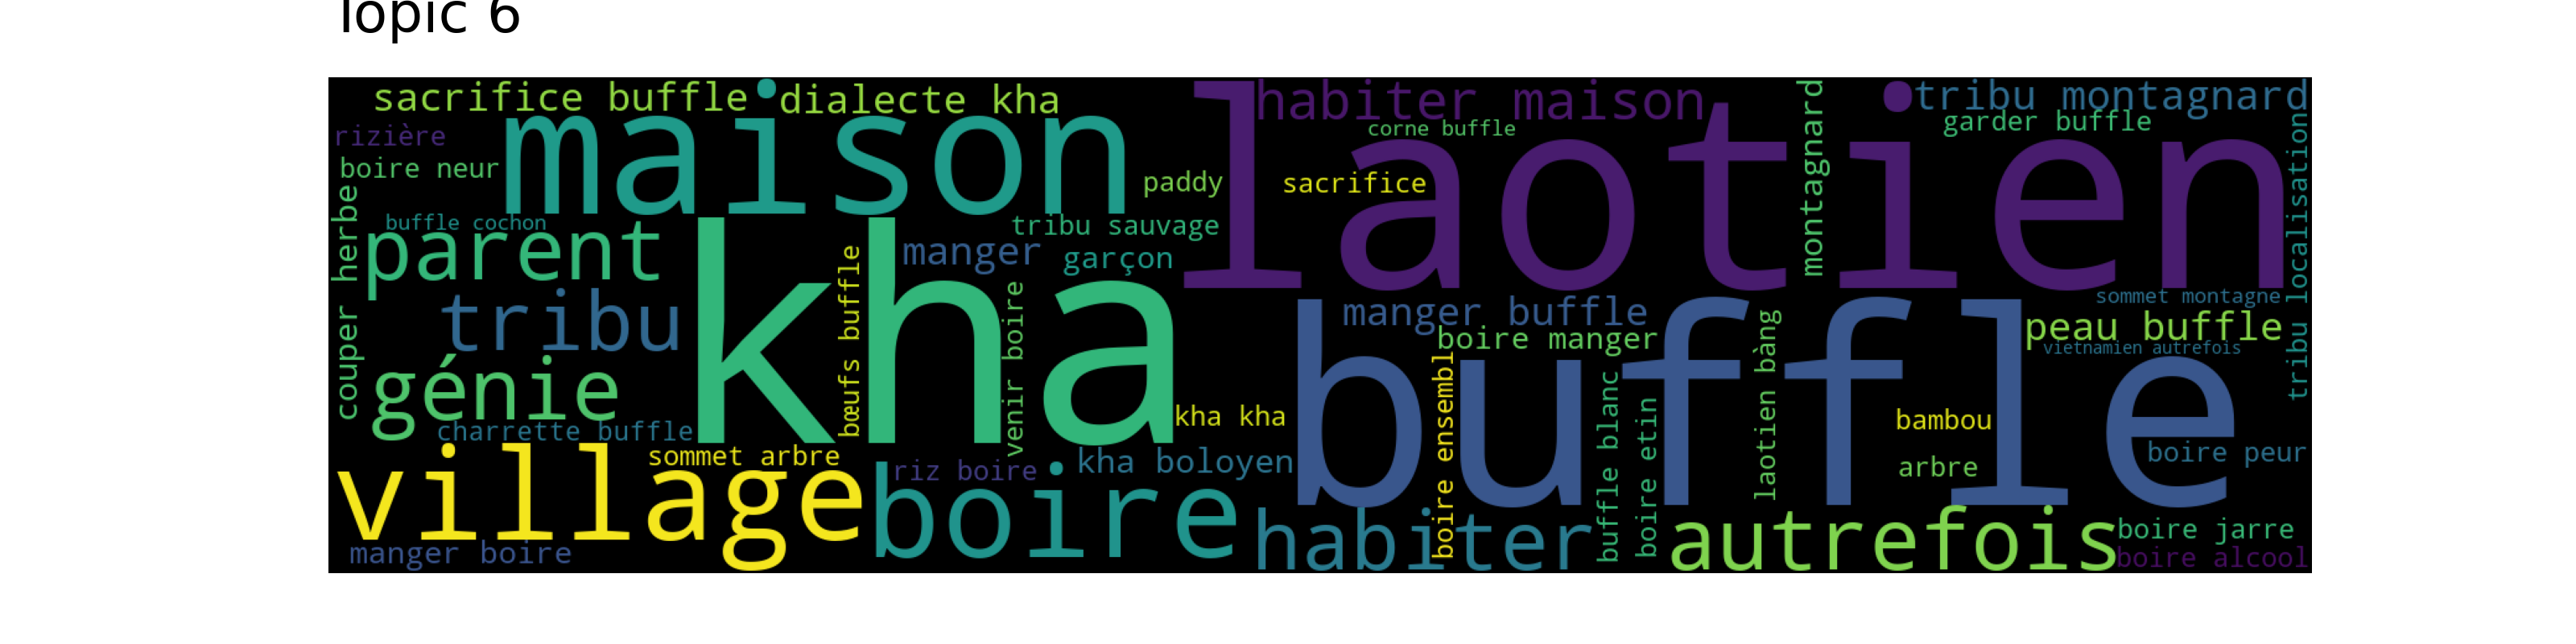
\includegraphics[width=\textwidth]{img/wordcloud model ngram 200 topic 6 .png}
         \caption{Les ethniques Vietnamiens/Laotiens}
         \label{fig:tp12_6}
     \end{subfigure}
     \hfill
        \caption{Les sujets de Laos/ Cambodge}
        \label{fig:lao_cam}
\end{figure}

La Figure \ref{fig:vie_chn} met en évidence deux groupes de documents qui sont regroupés principalement en fonction des langues autres que le français qui coexistent dans les textes. Dans ce cas, le modèle tient compte de la présence de mots étrangers qui apparaissent fréquemment, plutôt que du contenu réel des sujets. Dans le nuage de mots des documents chinois, on trouve de nombreux noms en Pinyin qui n'apportent aucune signification. Cependant, il y a deux mots clés importants, "graver" et "antique", qui proviennent d'un grand article sur la sigillographie chinoise. Malheureusement, il y a également de bons articles sur la médecine traditionnelle et des récits sur les rois vietnamiens qui sont mal classés dans la liste des documents.

\begin{figure}[h]
     \centering
     \begin{subfigure}[b]{.9\textwidth}
         \centering
         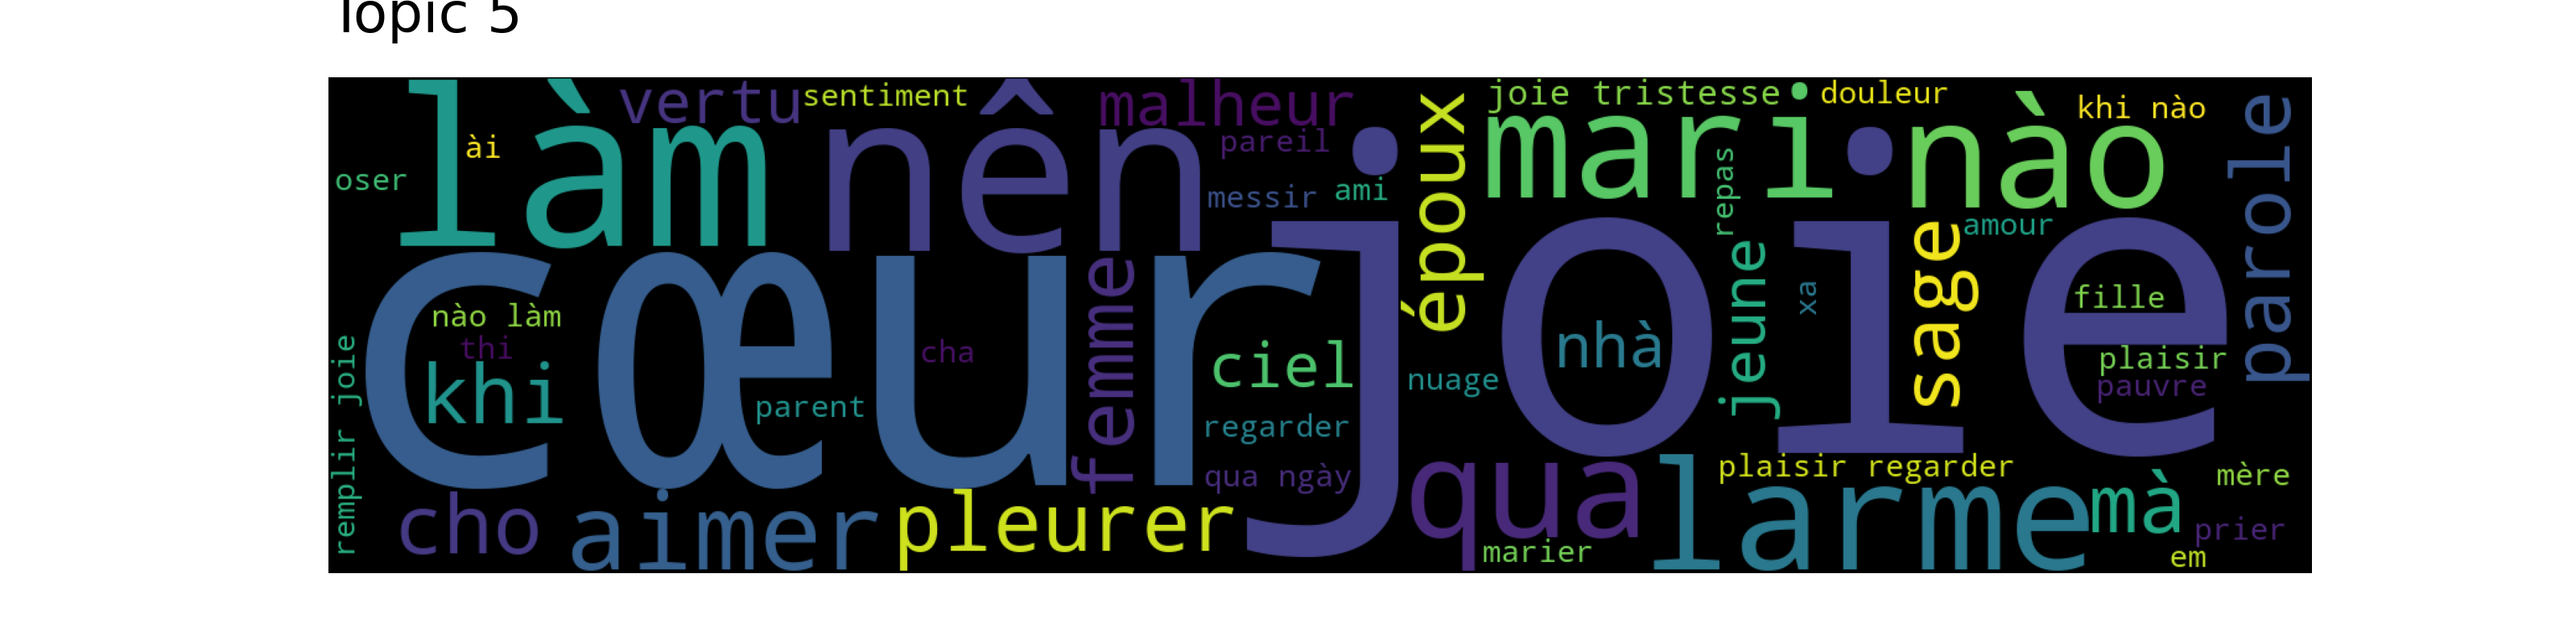
\includegraphics[width=\textwidth]{img/wordcloud model ngram 200 topic 5 .png}
         \caption{Traduction/Bilingue Vietnamien}
         \label{fig:tp12_5}
     \end{subfigure}
     \hfill
     \begin{subfigure}[b]{.9\textwidth}
         \centering
         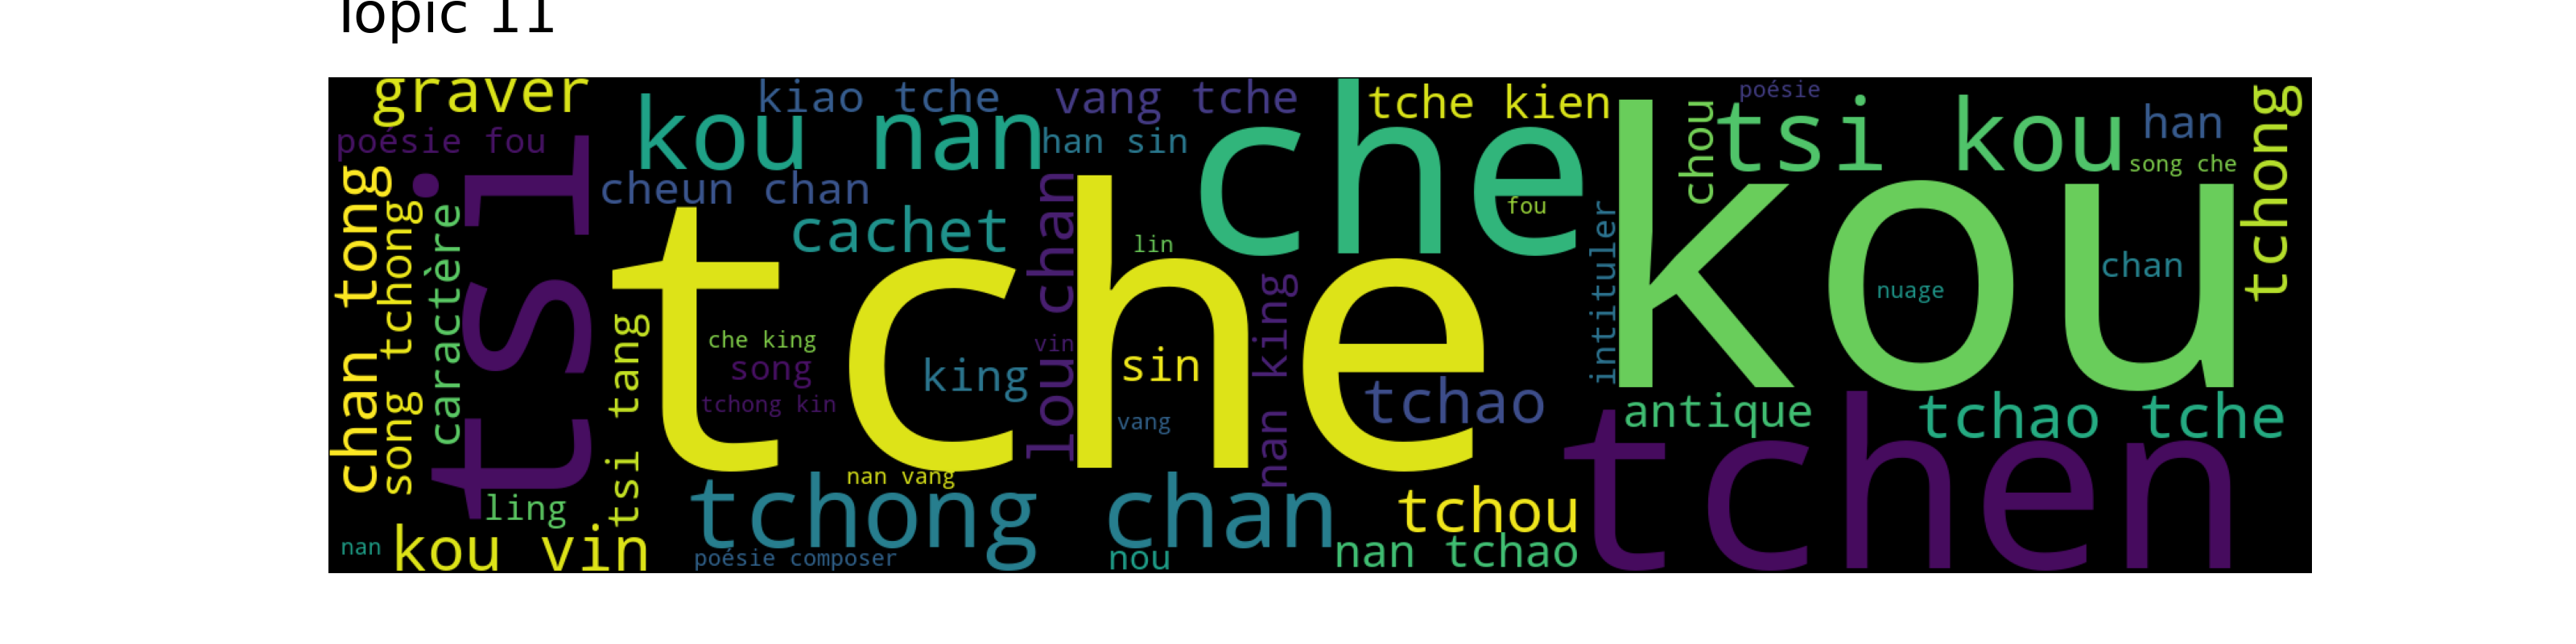
\includegraphics[width=\textwidth]{img/wordcloud model ngram 200 topic 11 .png}
         \caption{Traduction/Bilingue Chinoise}
         \label{fig:tp12_11}
     \end{subfigure}
     \hfill
        \caption{Les documents billingue ou les traductions}
        \label{fig:vie_chn}
\end{figure}

Un autre type de regroupement considéré comme un mauvais regroupement est illustré dans la Figure \ref{fig:noise_topic}, où le modèle a évalué des documents tels que les couvertures, les tables des matières, les avis, les listes de membres, les listes de sociétés correspondantes, ou encore les rapports d'activités trimestriels ou annuels de la société, comme des sujets principaux. Cela souligne également une faiblesse d'un modèle entraîné avec des bigrams, car il met en avant des collocations répétitives dans le texte, telles que "société de géographie", "directeur général", "activité de la société", alors que ces documents sont généralement courts et n'apportent pas suffisamment de contributions sémantiques. Nous considérons ces types de sujets comme du bruit.

\begin{figure}[H]
     \centering
     \begin{subfigure}[b]{0.9\textwidth}
         \centering
         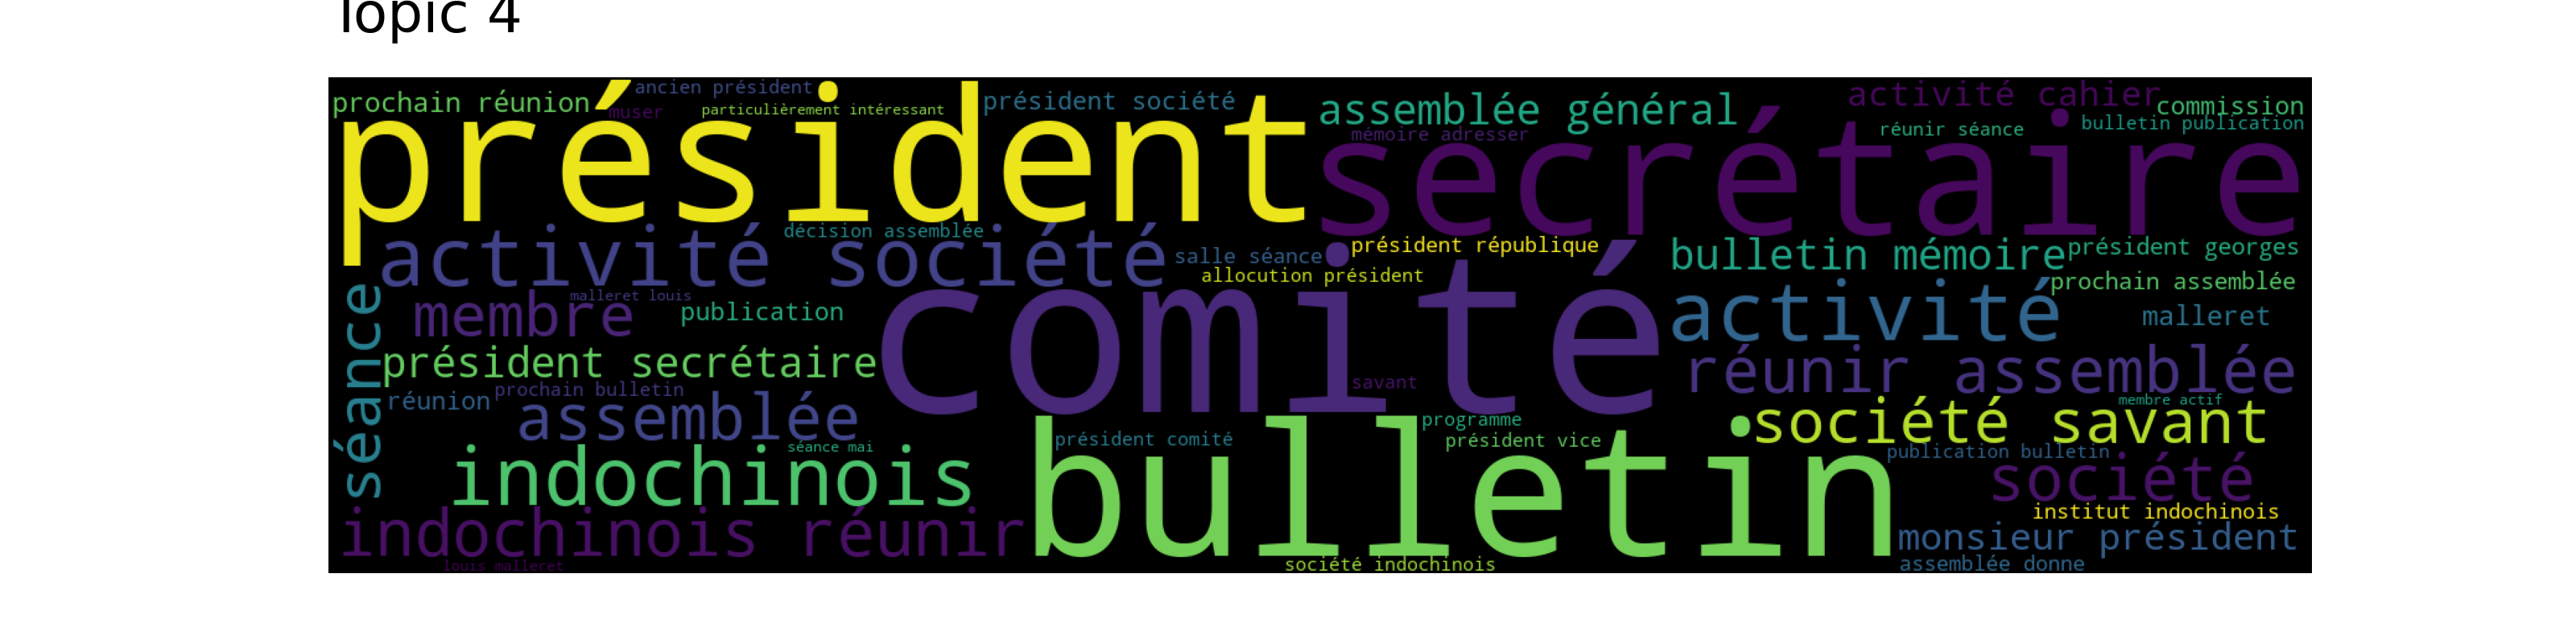
\includegraphics[width=\textwidth]{img/wordcloud model ngram 200 topic 4 .png}
         \caption{Assemblee generale, allocution president}
         \label{fig:tp12_4}
     \end{subfigure}
     \hfill
     \begin{subfigure}[b]{0.9\textwidth}
         \centering
         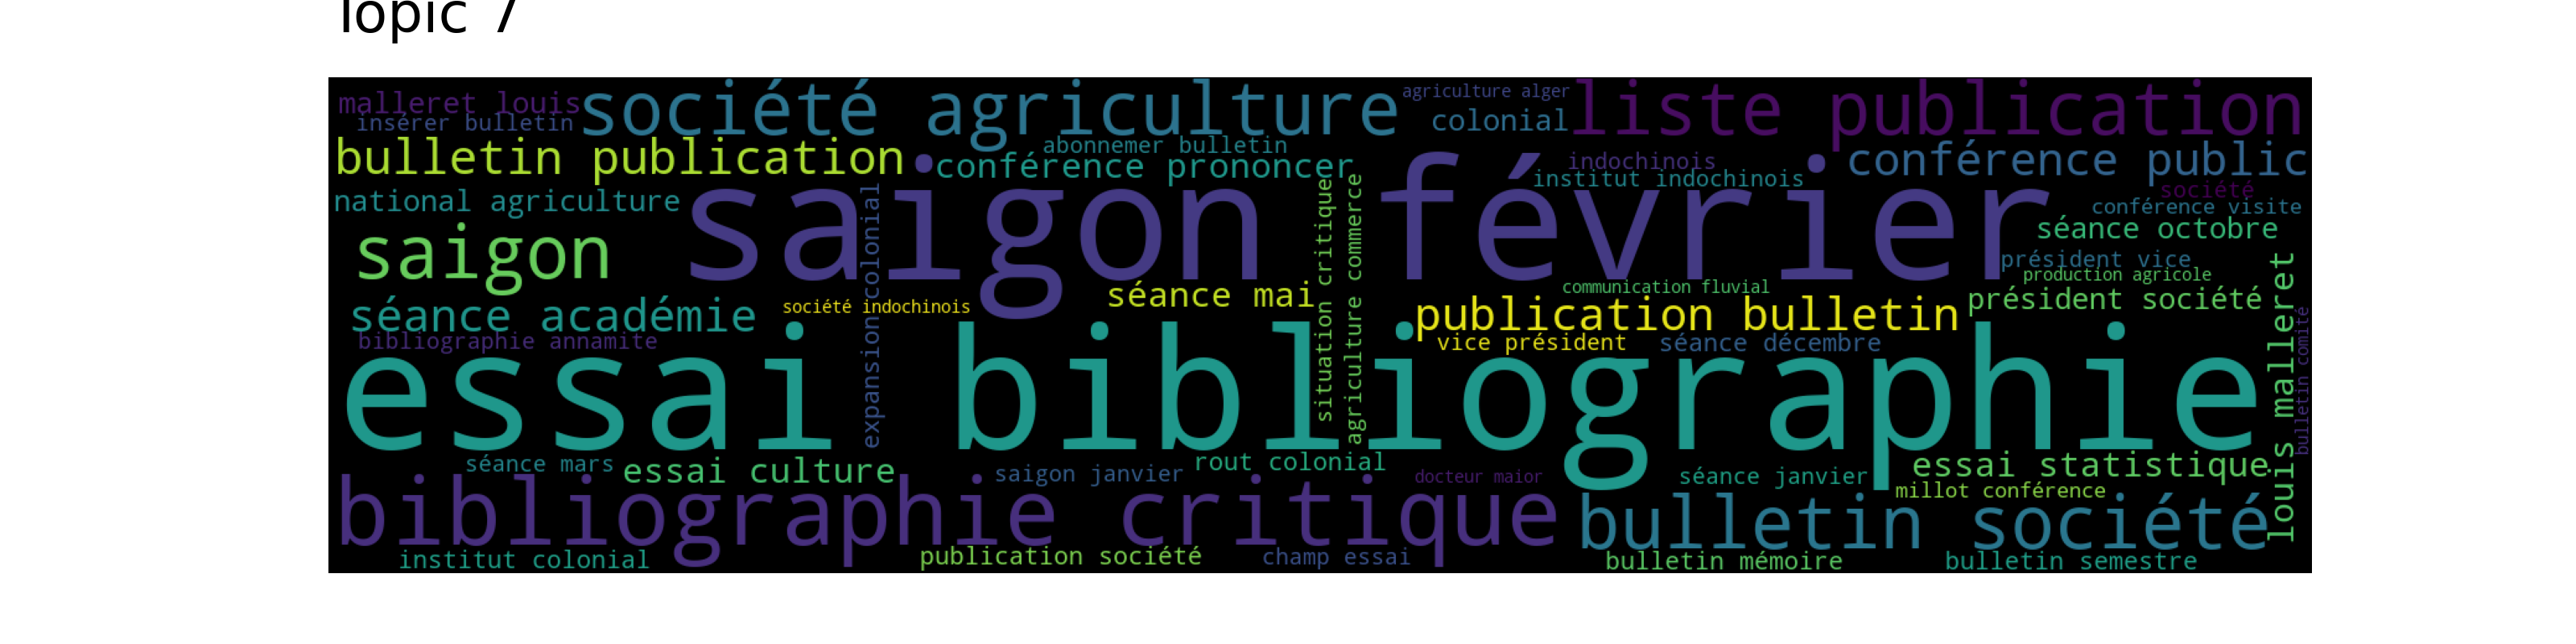
\includegraphics[width=\textwidth]{img/wordcloud model ngram 200 topic 7 .png}
         \caption{Couverture, tables de matiere, avis, liste des membres}
         \label{fig:tp12_7}
     \end{subfigure}
     \hfill
     \begin{subfigure}[b]{0.9\textwidth}
         \centering
         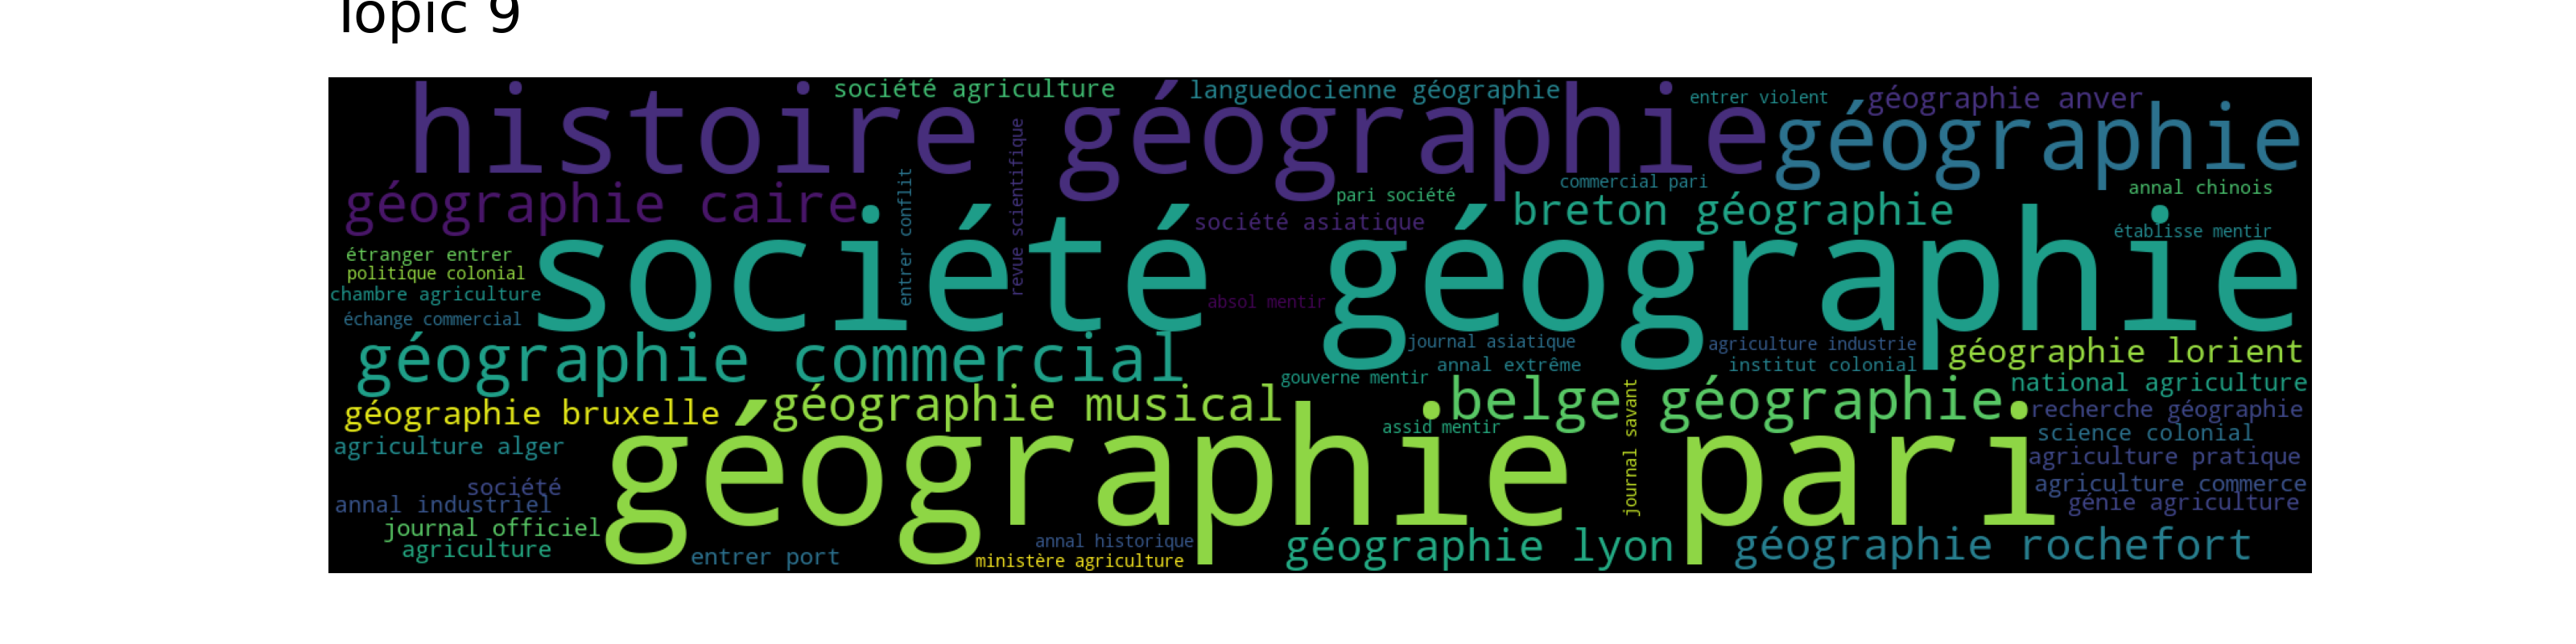
\includegraphics[width=\textwidth]{img/wordcloud model ngram 200 topic 9 .png}
         \caption{Catalogues, listes des correspondantes}
         \label{fig:tp12_9}
     \end{subfigure}
        \caption{Les sujets du bruit}
        \label{fig:noise_topic}
\end{figure}

Les vecteurs associés à chaque document peuvent être représentés visuellement en utilisant une projection UMAP, de manière similaire à ce qui est montré sur la Figure \ref{fig:umap12}. Dans cette représentation, les points symbolisent les segments et sont colorés en fonction de leur sujet principal. Une observation importante est la prédominance de quatre sujets principaux : "recherche générale", "agriculture et plantation", "militaire" et "architecture cambodgienne". Les vecteurs du sujet "recherche générale" se positionnent au centre de l'espace où l'on peut également trouver les vecteurs des autres groupes, un peu comme dans la zone des documents militaires. En revanche, les documents relatifs aux sujets "agriculture" et "architecture cambodgienne" sont assez distinctifs et se trouvent en périphérie de l'espace.

\begin{figure}[t]
    \centering
    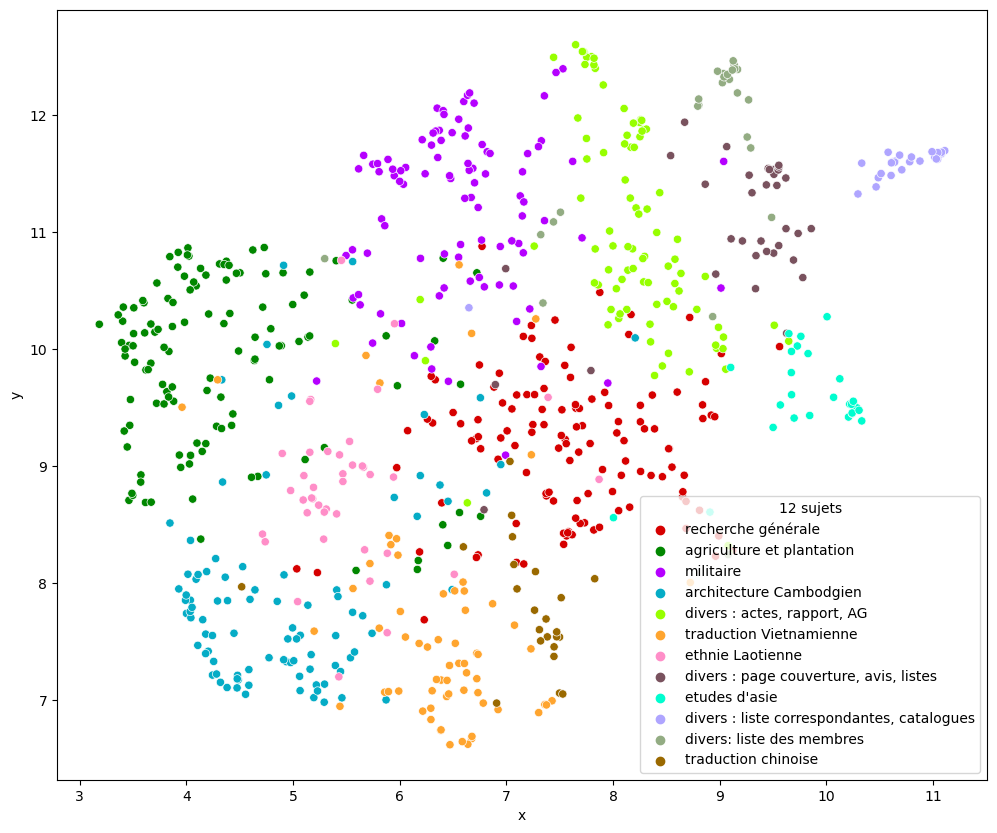
\includegraphics[width=13cm]{img/12umap.png}
    \caption{Distribution spatial des sujets}
    \label{fig:umap12}
\end{figure}

\subsection{Discussion}
Dans cette section, nous présentons deux modèles thématiques qui s'appliquent directement à notre corpus. Contrairement à LDA, une méthode traditionnelle que nous avions initialement envisagée pour la classification de documents, mais qui n'a pas produit de résultats clairs, Top2Vec a rapidement démontré sa supériorité en offrant une compréhension significative de la structure sémantique de ses thèmes. 

En conséquence, nous avons choisi d'exploiter Top2Vec pour approfondir nos recherches dans ce projet. Malgré une analyse approfondie des sujets, certaines limites subsistent. Notre objectif est donc de minimiser autant que possible les thèmes moins pertinents, afin de nous concentrer sur la sélection des textes les plus essentiels qui contribuent à la réputation de ce magazine.

En outre, un autre défi que nous rencontrons avec Top2Vec concerne la tendance des grands sujets à englober un large éventail de petits domaines de recherche, ce qui complique la création de sujets plus précis. Malgré nos nombreux essais avec différents paramètres, nous n'avons pas réussi à obtenir plus que le nombre correct de sujets. 

De plus, en dehors de quelques sujets principaux comme "Agriculture", "Militaire" ou bien "Architecture", chaque exécution de l'apprentissage automatique génère un modèle différent, ce qui pose des problèmes en termes de reproductibilité, similaire à de nombreux modèles d'apprentissage aléatoire. Notre tâche consistera donc à développer une méthodologie de recherche capable de systématiquement identifier les documents liés à chaque sous-thème de manière cohérente.

% Il est également intéressant d'examiner la répartition des sujets au fil du temps à l'époque, la figure \ref{fig:topic_time} présente cet aspect. On peut immédiatement remarquer une distribution inversée dans le temps entre le sujet 6 et le sujet 8. Le sujet 0, composé de sujets liés à l'histoire, à la recherche et à la littérature, est très rare avant 1920, lorsque la colonie indochinoise était encore en cours d'installation. Le sujet 6, qui concerne les traductions et les textes vietnamiens, n'apparaît que après les années 1945, tandis que le sujet 8, qui englobe les documents du gouvernement, se trouve principalement au début du régime colonial de l'époque. On peut également noter que le sujet militaire est plus concentré autour de l'année 1945, une période particulièrement importante de la guerre de libération au Vietnam et en Indochine. Les documents sur l'agriculture (sujet 1) sont moins présents entre 1910 et 1950.

% \begin{figure} %[!ht]
%     \centering
%     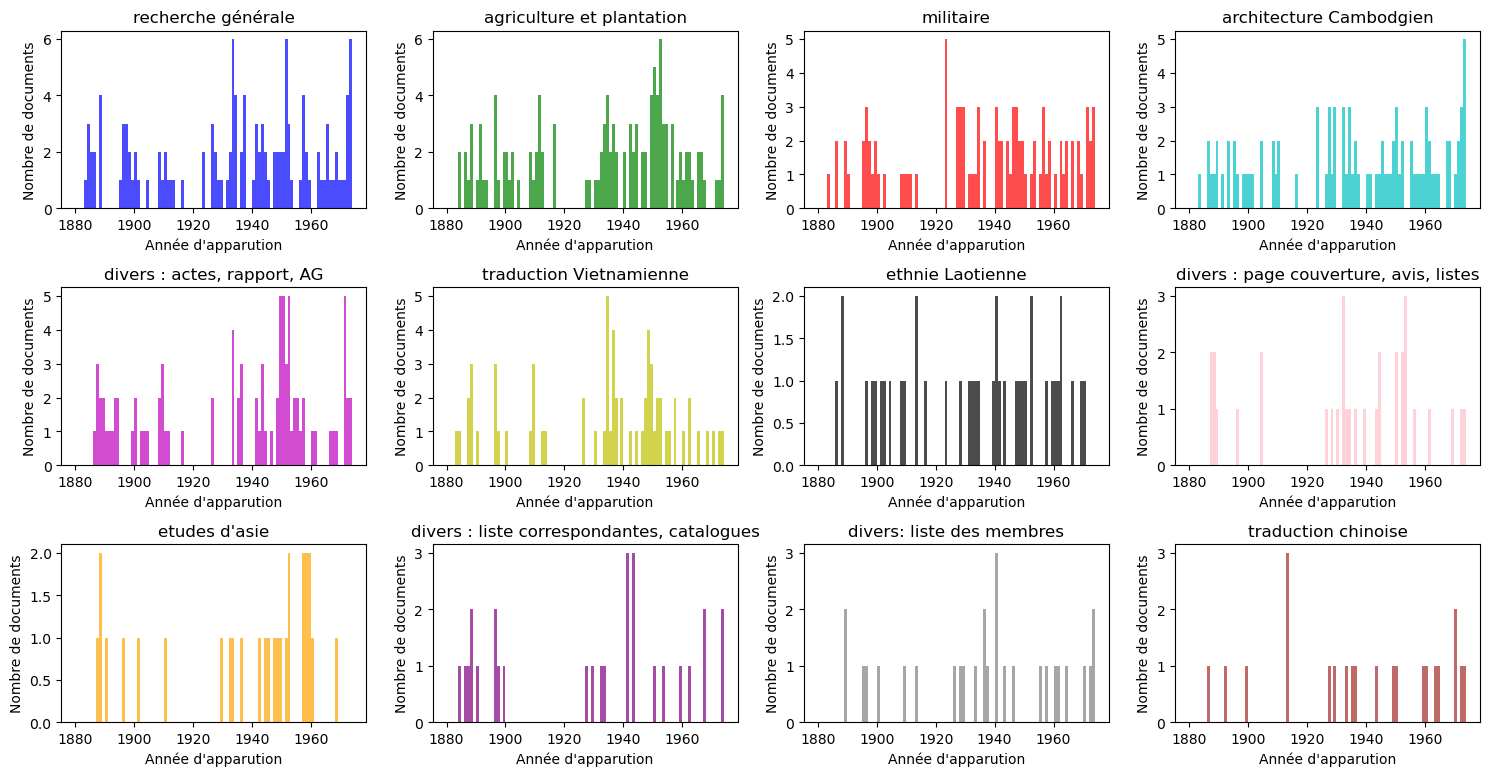
\includegraphics[width=14cm]{img/12temp.png}
%     \caption{Distribution temporelle des sujets}
%     \label{fig:topic_time}
% \end{figure}

\clearpage
\newpage
% \mbox{~}
% \clearpage
% \newpage

\section{Amélioration du modèle de regroupement}
Dans cette section, nous allons proposer deux approches pour améliorer le regroupement des sujets. La première approche est dirigée directement de nos observations quand nous avons constaté qu'une part importante des documents divers sont identifiés comme un sujet en raison de la répétition fréquente de certains vocabulaires ou de la similarité structurelle et de longueur entre ces documents. La présence de ces documents dans le corpus peut influencer le regroupement. Comme ces contenus de documents ne contribuent pas beaucoup de significations, nous avons décidé de les éliminer du corpus en les filtrant par les titres de documents. 

Les résultats de la première approche seront discutés, et il apparaît que le modèle n'arrive toujours pas à distinguer différentes disciplines scientifiques dans le corpus. Un autre problème réside dans les articles qui mélangent le français et une autre langue, souvent le vietnamien ou le chinois, et qui peuvent parfois inclure de véritables articles sur d'autres sujets.
C'est pourquoi nous proposons la deuxième approche, qui consiste à utiliser Word2Vec. Ce modèle est capable de rechercher une liste de mots-clés, et un modèle Top2Vec qui s'entraîne  sur un espace de mots plus large pourrait alors extraire les documents pertinents pour chaque mot-clé. 
Une analyse de cette méthode de recherche sera apportée en fin de la section.

\subsection{Avec un corpus pré-filtré}
\subsubsection{Suppression des documents moins pertinents}
Pour réduire l'impact des documents divers liés à l'administration ou à l'organisation de la société B.S.E.I, nous allons les filtrer avant de procéder à l'entraînement du corpus. Le tableau \ref{tab:acte_societe} présente une statistique sur la quantité de documents et de mots de ce type de documents. Cette partie représente 10,35 \% de l'ensemble du nombre de documents et 4,24 \% en termes de quantité de mots.
\begin{center}
\begin{tabular}{ |c|c|c| } %{|p{5cm}|p{5cm}|p{4cm}|}
\hline
Titre & Nombre de documents & pourcentage de mots\\
\hline
actes société & 45 & 1.34\%  \\ 
liste membres & 22 &  2.22\%  \\
liste générale membres & 15 & 0.37\%  \\
procès verbaux/verbal & 57 & 0.29\% \\ 
bureau-de-la-société & 15 & 0.37\%  \\
\hline
Total & 139 & 4.24\%  \\
\hline
\end{tabular}
\label{tab:acte_societe}
\end{center}

\subsubsection{Analyse des résultats}

Le modèle a ensuite été ré-entraîné, ce qui a abouti à une nouvelle modélisation réduite à 6 sujets, avec les mots-clés qui sont répertoriés dans le tableau \ref{tab:6topic}.

\begin{center}
\begin{tabular}{|p{15cm}|}
\hline
Regroupement des sujets et les mot-cles\\
\hline
 Sujet 0 : centimètre, sécher, sec, couche, acide, sol, liquide, graine, rendement, quantité, humidité, température, mètre, surface, tige \\ \hline
 Sujet 1 : joie, larme, prosterner, malheur, cœur, ciel, écria, parole, pleurer, époux, mari, messir, hsiuan, bouddha, bonheur \\ \hline
 Sujet 2 : chercheur, pensée, civilisation, savant, synthèse, intellectuel, science, conception, spécialiste, ouvrage, documentation, morale, scientifique, lecteur, connaissance \\ \hline
 Sujet 3 : amiral, frégate, expédition, capitaine, canonnière, navire, marine, commandant, prise, débarquer, artillerie, expéditionnaire, colonie, occupation, conquête \\ \hline
 Sujet 4 : conférence, culturel, indochinois, président, activité, société, étude, comité, membre, programme, savant, ecole, congrès, secrétaire, bibliothèque \\ \hline
 Sujet 5 : monument, sculpture, statue, relief, sanctuaire, angkor, khmèr, décoratif, édifice, linteau, architecture, art, temple, buddha, prei \\ \hline
 Sujet 6 : géographie, société, agriculture, journal, revue, rulletin, society, indo, annal, colonial, bulletin, savant, colonie, commercial, courrier \\ \hline
\end{tabular}
\label{tab:6topic}
\end{center}
% \vspace{1cm}

Le modèle a réussi à former une structure de sujets avec une répartition de documents plus équilibrée, comme le montre la Figure \ref{fig:repartition_7topics}. En observant la répartition en nombre de mots, on constate que les deux sujets "Vie et Religieux" et "Militaire" contiennent beaucoup plus de texte que les autres sujets. En effet, parmi les documents du sujet "Militaire", on a trouvé que deux sur trois étaient de grandes traductions du roman historique "Les Trois Royaumes", qui relate une longue période de guerre en Chine et qui est classé parmi les romans les plus longs et les plus anciens de l'histoire chinoise.

\begin{figure*}[]
    \centering
    \begin{subfigure}[t]{0.45\textwidth}
        \centering
        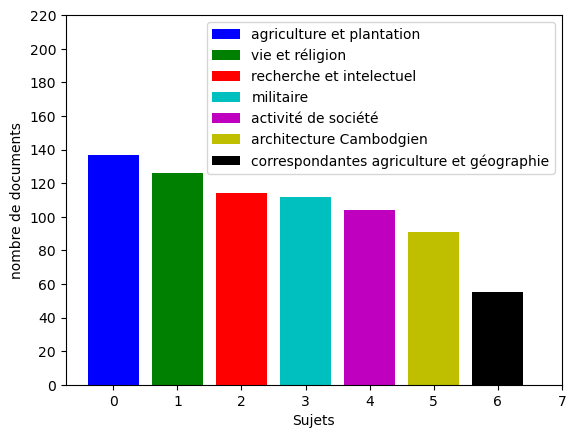
\includegraphics[height=1.9in]{img/6topic_size_docs.png}
        \caption{Répartition de documents}
    \end{subfigure}%
    ~ 
    \begin{subfigure}[t]{0.45\textwidth}
        \centering
        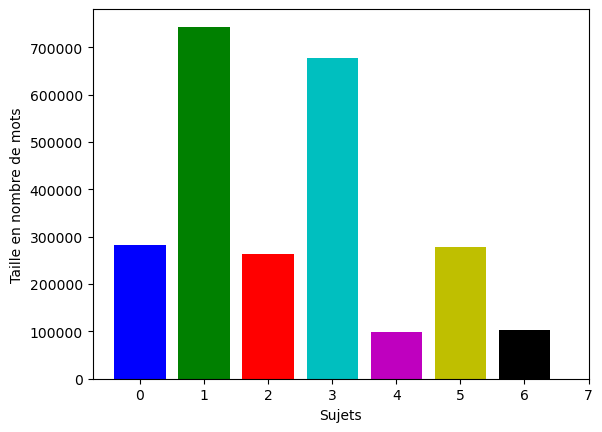
\includegraphics[height=1.9in]{img/6topic_size_words_true.png}
        \caption{Répartition de mots}
    \end{subfigure}
    \caption{Répartition entre les sujets}
    \label{fig:repartition_7topics}
\end{figure*}

En revanche, les documents liés aux activités et aux sociétés correspondantes contiennent très peu de texte dans leurs documents mais malgré tout ils sont bien regroupés par la similarité de leur nature et aussi de leur vocabulaire.

% \begin{figure}[H] %[!ht]
%     \centering
%     \includegraphics[width=14cm]{img/wordcloud filter 2 model ngram 200 topic 0 .png}
%     \caption{WordCloud du sujet }
%     \label{tp0}
% \end{figure}

\begin{figure}[H] %[!ht]
    \centering
    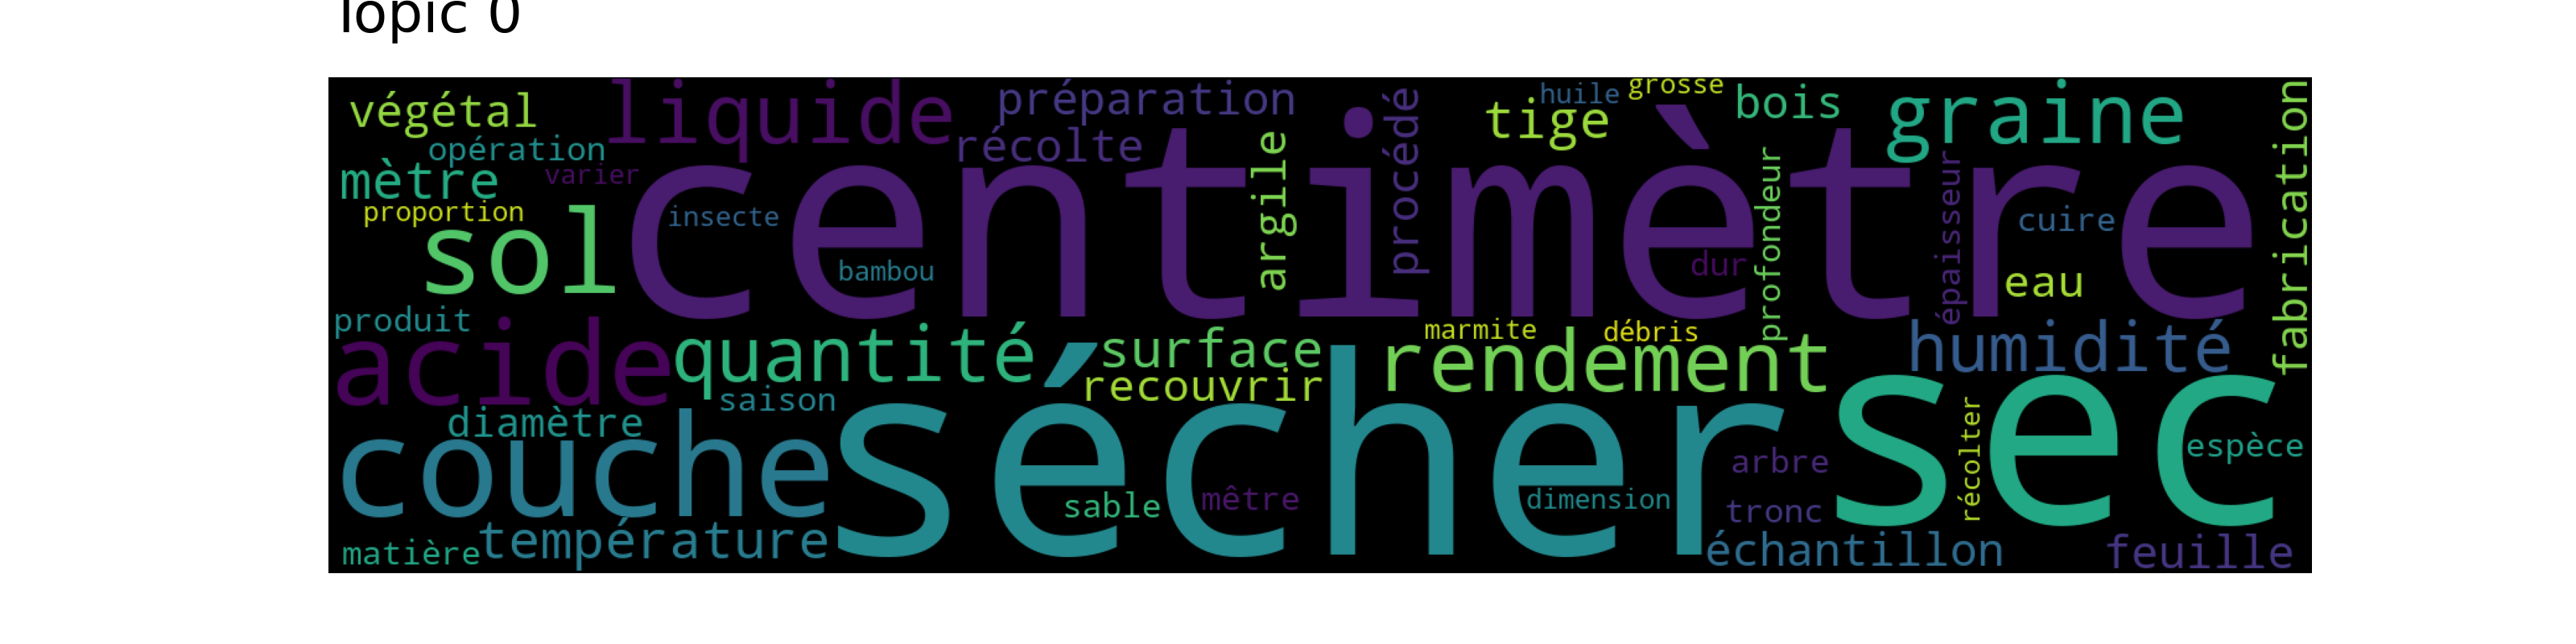
\includegraphics[width=14cm]{img/final_6_topic 0 .png}
    \caption{Agriculture, plantation, alimentation }
    \label{tp0}
\end{figure}
\textbf{Topic 0}: Agriculture, plantation, alimentation\newline
Quelques documents de référence  : 
\begin{itemize}
    \item 
Etudes des minéraux lourds de quelques sables littoraux par Hoang Ngoc Can 1964
    \item 
Résultats des mesures de la température des eaux marines par Hoang Ngoc Can 1964

    \item 
Au sujet des tectes de Dalat par Mailles 1934
    \item 
Compte rendu analytique sur les courants terrestres par Lourme 1883

    \item 
Rapport sur la fabrication de l'acool de riz en Cochinchine par Lévie 1883

    \item 
L'industrie du décortiage du riz en Basse-Cochinchine par Passerat de la Chapelle 1901

    \item 
La poterie dans le Sud-Cambodge par A. Souyris Rolland 1950
\end{itemize}

Les nuages de mots associés à chaque sujet reflètent de manière cohérente l'identité de chaque sujet. En effet, le Bulletin du Comité agricole et industriel de la Cochinchine, en tant que prédécesseur, avait une orientation centrée sur l'agriculture et la culture, et ces thèmes continuent de prédominer dans l'ensemble du corpus. Le premier thème, en particulier, est composé d'articles scientifiques axés sur la recherche en agriculture en Indochine. Les mots-clés révèlent une diversité de cultures tropicales, ainsi que des éléments naturels fondamentaux tels que le sol, l'eau, le sable, la saison, l'argile, la température de surface et leurs caractéristiques telles que "sec", "humidité", "acide", "profondeur", "sécheresse", etc. De plus, on trouve des termes liés au processus de production agricole, tels que "préparation", "fabrication", "récolte", "récolter", qui renforcent la cohérence thématique de ce sujet.

% Effectivement, le thème général de l'agriculture couvre une grande variété de nuances et de domaines d'études plus spécifiques qui ne sont pas facilement discernables à partir d'un simple nuage de mots. Les termes techniques tels que "centimètre", "quantité", "diamètres", "dimension", "échantillon" suggèrent une dimension de précision et de mesure au sein de ce domaine.

Il est important de noter que derrière ce sujet général de l'agriculture, il existe des sujets plus spécialisés et des sous-domaines qui nécessitent une recherche plus approfondie pour être pleinement compris. Par exemple, au sein de cette thématique, il est possible de trouver des recherches portant sur les matériaux, l'industrie, voire des aspects tels que l'artisanat, comme la fabrication de céramique. Ces sujets plus spécifiques et ces nuances offrent d'excellents points de référence dans le corpus. Cependant, une analyse plus détaillée et approfondie est nécessaire pour explorer les thèmes sous-jacents et comprendre pleinement la portée de la recherche dans le domaine de l'agriculture en Indochine.

\begin{figure}[H] %[!ht]
    \centering
    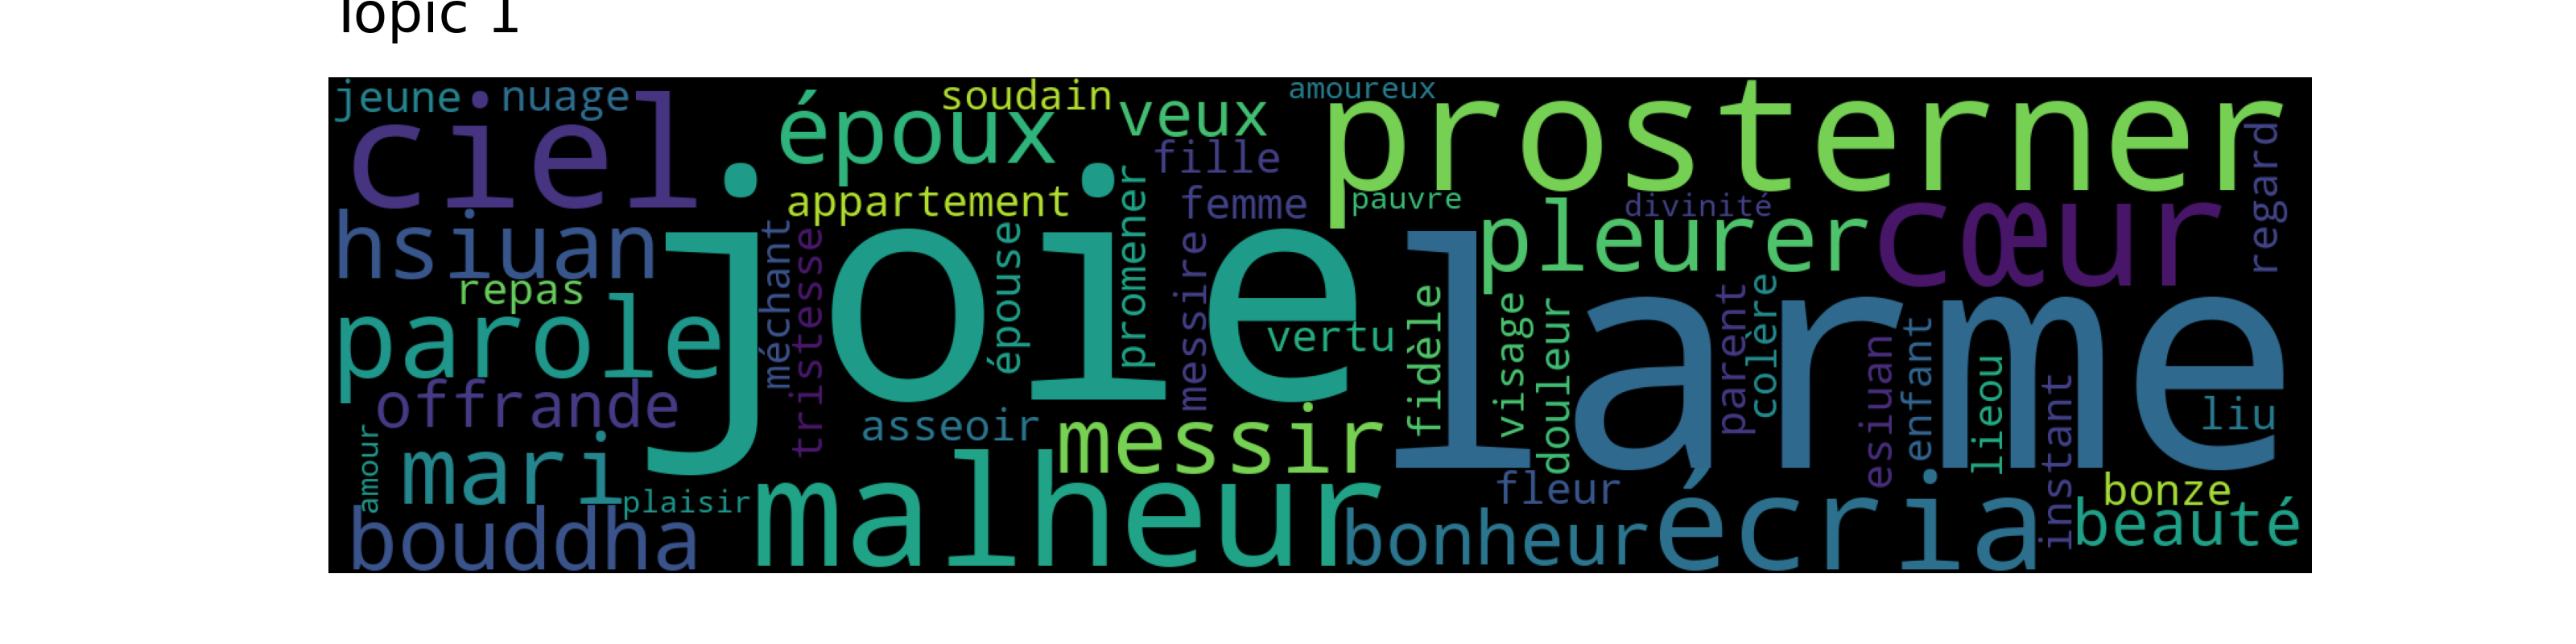
\includegraphics[width=14cm]{img/final_6_topic 1 .png}
    \caption{La vie de famille et religion }
    \label{tp1}
\end{figure}

Topic 1 : La vie de famille et religion

Le bouddhisme et le culte des ancêtres représentent deux des croyances fondamentales du peuple vietnamien, et ils sont intrinsèquement liés à la structure familiale vietnamienne. Les récits et les enseignements religieux sont fréquemment ancrés dans la vie familiale et les émotions humaines. Bien que l'analyse des mots puisse suggérer une prédominance de termes liés aux émotions et à la famille, en réalité, la plupart des articles sur ce sujet sont associés à la dimension religieuse.

"L’Islam est professé par 2\% de la population, 6\% confessent le chris-tianisme et 92\% le bouddhisme. Cette dernière religion est surtout répandue au Camboge et au Laos ; au Viet-Nam, elle est imprégnée de confucianisme"\footcites{truong}


- Topic 2: Intellectuel
\begin{figure}[H] %[!ht]
    \centering
    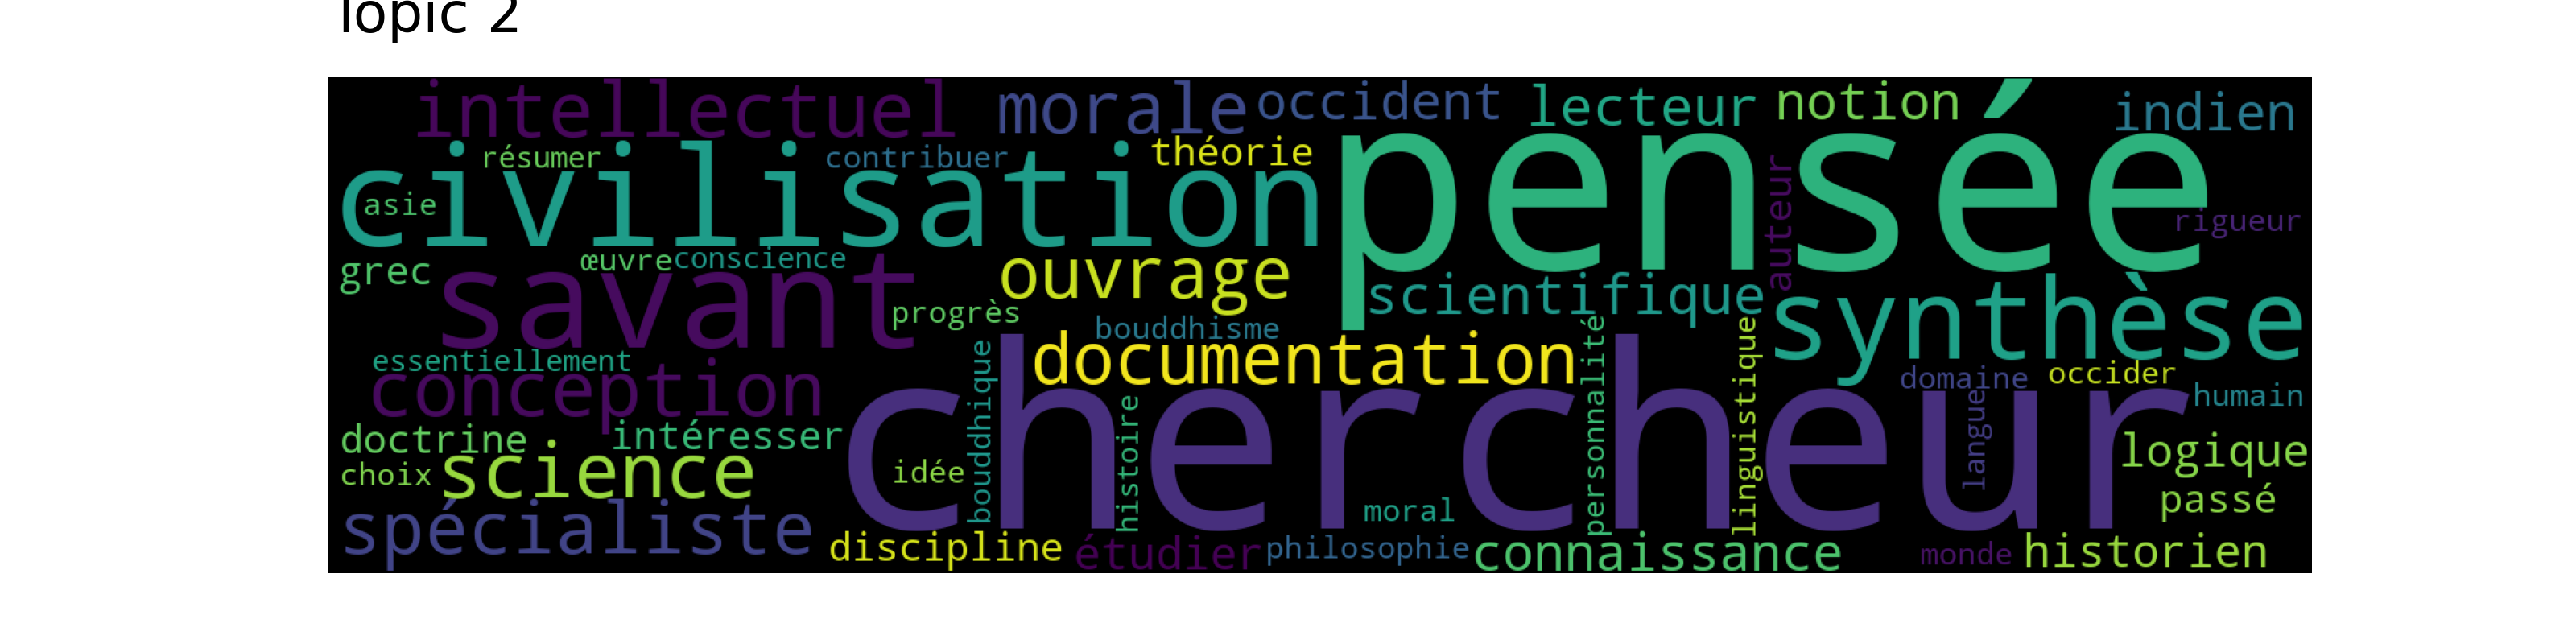
\includegraphics[width=14cm]{img/final_6_topic 2 .png}
    \caption{Intellectuel }
    \label{tp2}
\end{figure}

B.S.E.I reste est une société "savante", car cette expression occupe une place importante dans le deuxième thème du corpus. Ce sujet comprend des sujets intellectuels et scientifiques, des recherches, des essais et des critiques sur l'Indochine. Les discussions tournent autour de sujets autres que l’agriculture
"ouvrage", "documentation", "savant", "intellectuel",  "chercheur", "science", "pensée", "connaissance", "scientifique", "science", synthèse"

Effectivement, il est clair que le B.S.E.I avait un objectif scientifique bien défini et qu'il ne se limitait pas seulement aux articles de recherche scientifique. Il englobait également d'autres types de documents tels que les bibliographies, les catalogues, les publications de l'association et d'autres sociétés savantes. Cette approche montre que le journal avait une vision holistique de la recherche dans l'environnement scientifique et intellectuel de son époque.

En maintenant un réseau complet de documents intellectuels et en répertoriant de manière détaillée les travaux d'autres sociétés savantes, le B.S.E.I a contribué à enrichir les connaissances de ses membres et à promouvoir de nouvelles recherches dans le domaine de l'Indochine. Il a ainsi joué un rôle important dans la diffusion des connaissances et dans la création d'une communauté scientifique dynamique et productive.

Cela montre également que la revue ne se limitait pas à un seul domaine de recherche, mais embrassait une variété de sujets liés à l'Indochine, ce qui contribuait à sa richesse et à sa diversité scientifiques.
Il est important de noter que le magazine restait constamment au courant des développements scientifiques extérieurs et s'efforçait de maintenir son niveau. Cette approche témoigne de l'engagement de la société savante S.E.I. envers la recherche scientifique de haute qualité et son désir de rester à la pointe des avancées dans divers domaines liés à l'Indochine.

En restant à jour avec les développements scientifiques extérieurs, le magazine pouvait non seulement informer ses membres des dernières découvertes et avancées, mais aussi contribuer à la diffusion de ces connaissances au sein de la communauté scientifique indochinoise. Cela renforçait sa réputation en tant qu'organe de diffusion de la connaissance de premier plan dans la région.

En fin de compte, cette approche de maintien du niveau et d'ouverture aux développements extérieurs a contribué à faire du B.S.E.I une revue scientifique de grande qualité et à renforcer son rôle dans la promotion de la recherche en Indochine.

- Topic 3: Militaire
\begin{figure}[H] %[!ht]
    \centering
    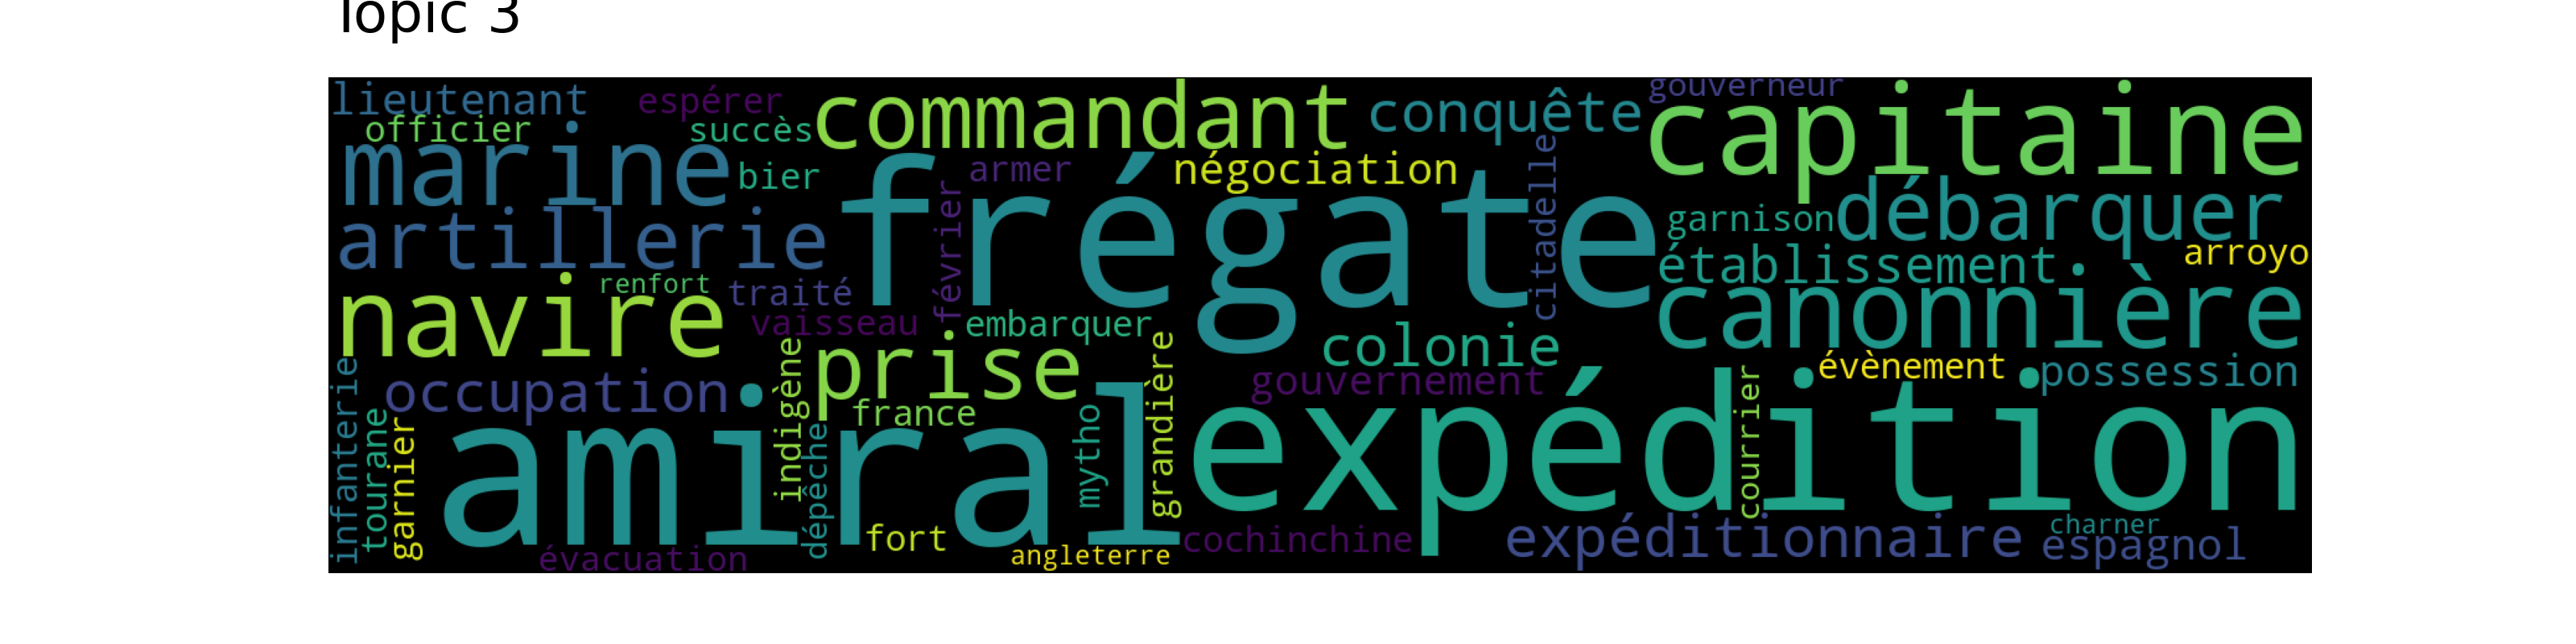
\includegraphics[width=14cm]{img/final_6_topic 3 .png}
    \caption{Document militaire et de la guerre}
    \label{tp3}
\end{figure}

Il est en effet intéressant de noter que, malgré le contexte colonial et les conflits qui ont marqué l'histoire de l'Indochine, la revue B.S.E.I a maintenu une politique de ne pas discuter de politique et de religion. Cela témoigne de sa volonté de se concentrer sur des sujets scientifiques et de recherche, plutôt que de s'engager dans des débats politiques ou religieux.

Le fait que les thèmes liés au militaire dans le nuage de mots comprennent principalement des études sur l'histoire de l'Indochine, les relations passées et les guerres avec les pays voisins est également intéressant. Cela montre que le journal a abordé ces sujets d'un point de vue historique et académique, plutôt que de prendre position sur des questions politiques contemporaines.

Il est également notable que des séries telles que Les trois royaumes ont été abordées dans le journal, ce qui démontre la diversité des sujets traités dans B.S.E.I et son engagement envers la recherche et la diffusion des connaissances purement scientifiques sur l'Indochine.

\begin{figure}[H] %[!ht]
    \centering
    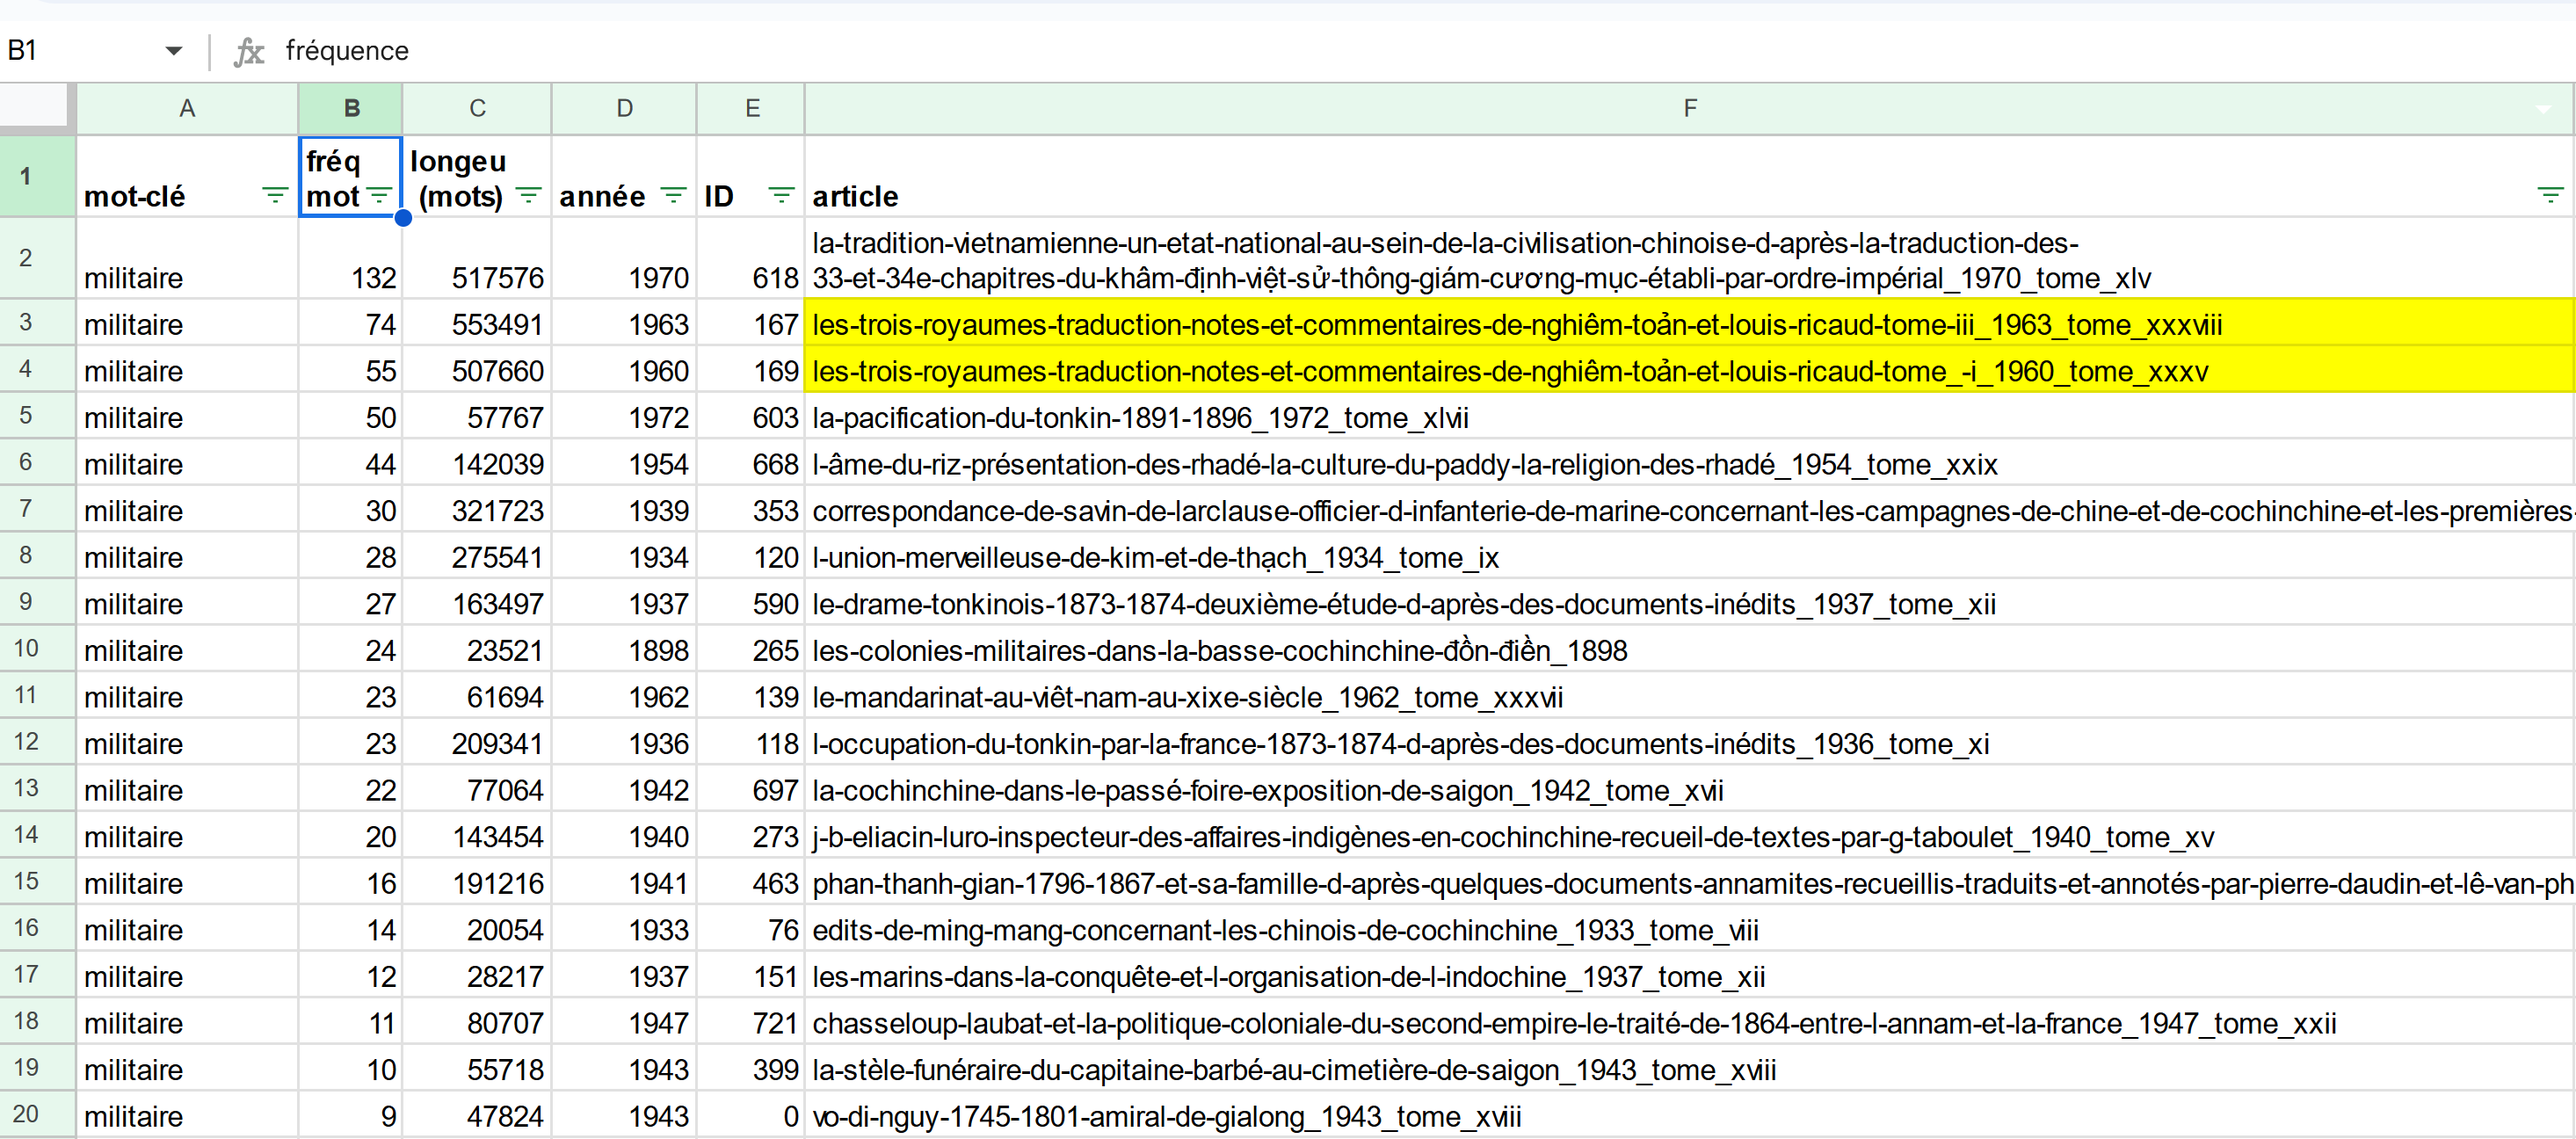
\includegraphics[width=1\linewidth]{img/millitaire.PNG}
    \caption{Enter Caption}
    \label{fig:enter-label}
\end{figure}

- Topic 4:  Activités administratives et intellectuelles de la société
\begin{figure}[H] %[!ht]
    \centering
    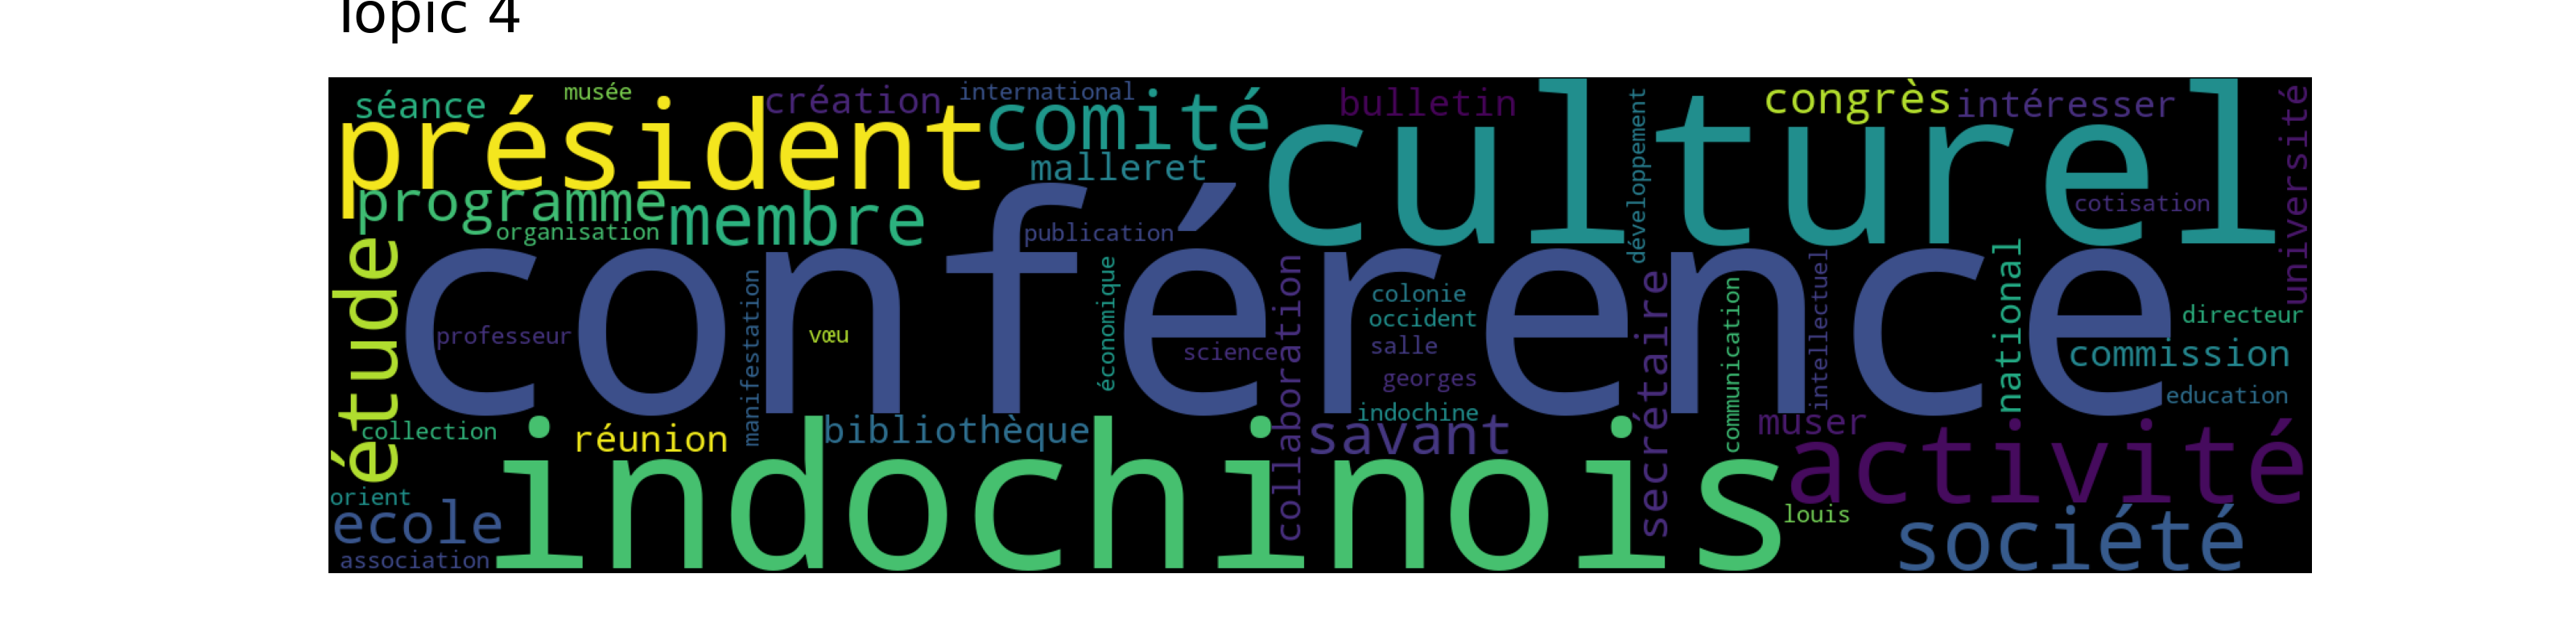
\includegraphics[width=14cm]{img/final_6_topic 4 .png}
    \caption{Activités administratives et intellectuelles de la société }
    \label{tp4}
\end{figure}

En plus de la rédaction d'articles, la société savante s'engage également dans d'autres activités scientifiques importantes telles que l'organisation de séminaires, de réunions, de congrès, de programmes, de séances et de commissions. Toutes ces activités contribuent à enrichir les intérêts de l'organisation et à promouvoir la recherche scientifique. Elles sont regroupées sous un thème distinct qui met en lumière leur importance au sein de la société savante.


- Topic 5: Architecture cambodgien  - Angkor Vat

\begin{figure}[H] %[!ht]
    \centering
    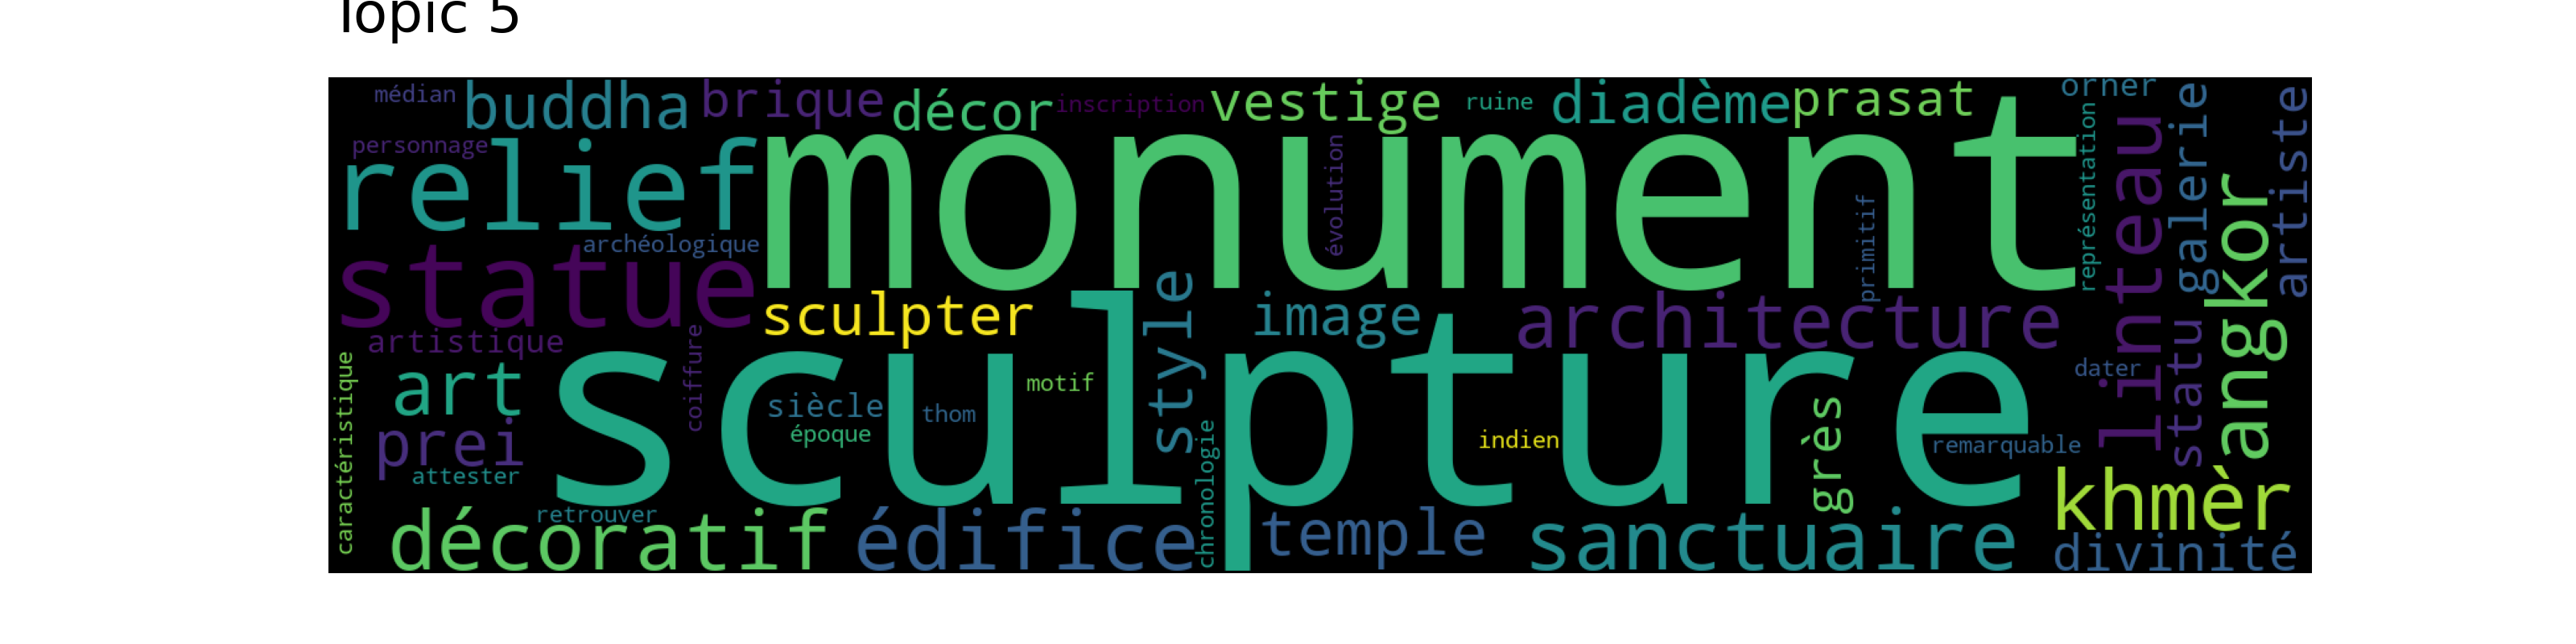
\includegraphics[width=14cm]{img/final_6_topic 5 .png}
    \caption{Architecture cambodgien }
    \label{tp5}
\end{figure}
L'architecture khmère et ses mystères ont toujours captivé l'attention des chercheurs indochinois. Dans lesquels, nous avons trouvé Angkor Wat qui est l'un des monuments emblématiques de l'architecture cambodgienne et l'un des sites historiques et religieux les plus importants au Cambodge.

« sculpture », « monument », « angkor », « décoratif », « khmer », « relief », « santuaire », « angle, « dégager », « statue », « divinité », « motif », «style », "temple", "édifice"

Bien que la plupart des recherches portent sur le Vietnam, en particulier sur la Cochinchine, il existe une exception notable en ce qui concerne les monuments et l'architecture. En observant le tableau de répartition ci-dessous, on peut voir que ce domaine, représenté en rose, suscite un intérêt particulièrement élevé au sein de la société savante. Les aspects artistiques de ces œuvres architecturales ont été étudiés en profondeur, avec une fréquence élevée, surtout dans les années 1950, et ce jusqu'aux derniers numéros. 

Ce tableau montre clairement que l'expertise dans le domaine de l'architecture des temples au Cambodge a évolué et s'est développée au fil du temps, passant d'une connaissance limitée à une compréhension approfondie, et cette expertise a été maintenue au fil des ans.
\begin{figure}[H] %[!ht]
    \centering
    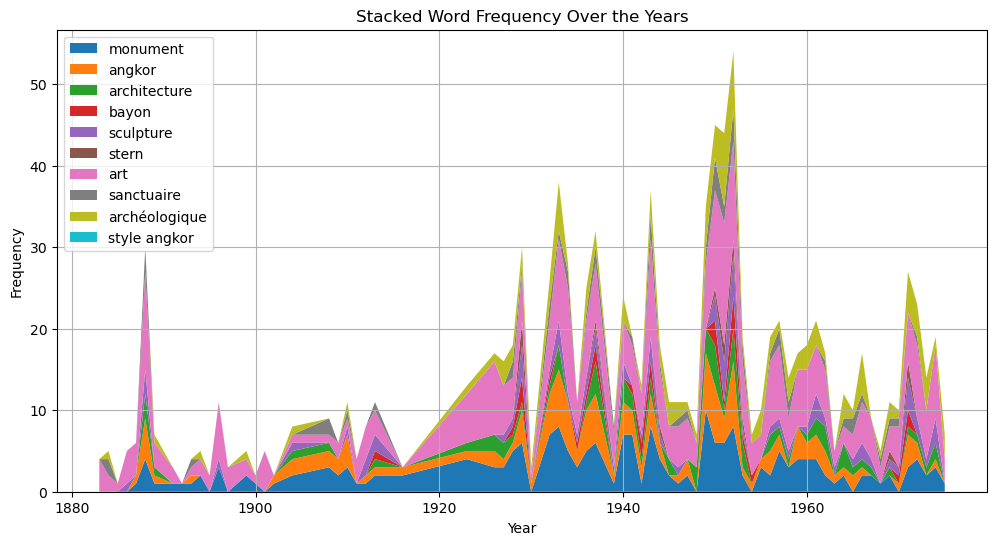
\includegraphics[width=14cm]{img/stackfreq_year_keyword_cambodge.png}
    \caption{Fréquence mots de l'architecture cambodgien}
    \label{stackfreq_year_keyword_cambodge}
\end{figure}

L'un des auteurs éminents qui a contribué aux recherches sur l'architecture des temples au Cambodge est Henri Marchal (1876-1970),un architecte français, mais aussi un explorateur, un archéologue et un philologue et épigraphe affecté à la Conservation d'Angkor.

Parmi les articles sur ce sujet, on peut citer :
\begin{itemize}
    \item 
L'art cambodgien moderne par H. Marchal (1913)

    \item 
Des influences étrangeres dans l'art de la civilisation khmers par H. Marchal (1936)

    \item 
Sur l'architecture de l'art Khmer primitif du Founan par H. Parmentier (1933)

    \item 
Le Naga dans l'art Khmer par H. Marchal (1937)

    \item 
Evolution du diademe dans la statuaire khmer par J. Boiseelier (1950)

    \item 
Note sur les alignements khmers par P. Paris (195é)

    \item 
Les travaux de la Conservation d'Angkors par H. Marchal (1953)

    \item 
Reconnaissance de l'ancienne chausssée khmer d'Angkor au Mékong par Kompong (1904)
\end{itemize}

- Topic 6: Correspondantes d'agriculture et de geographie

\begin{figure}[H] %[!ht]
    \centering
    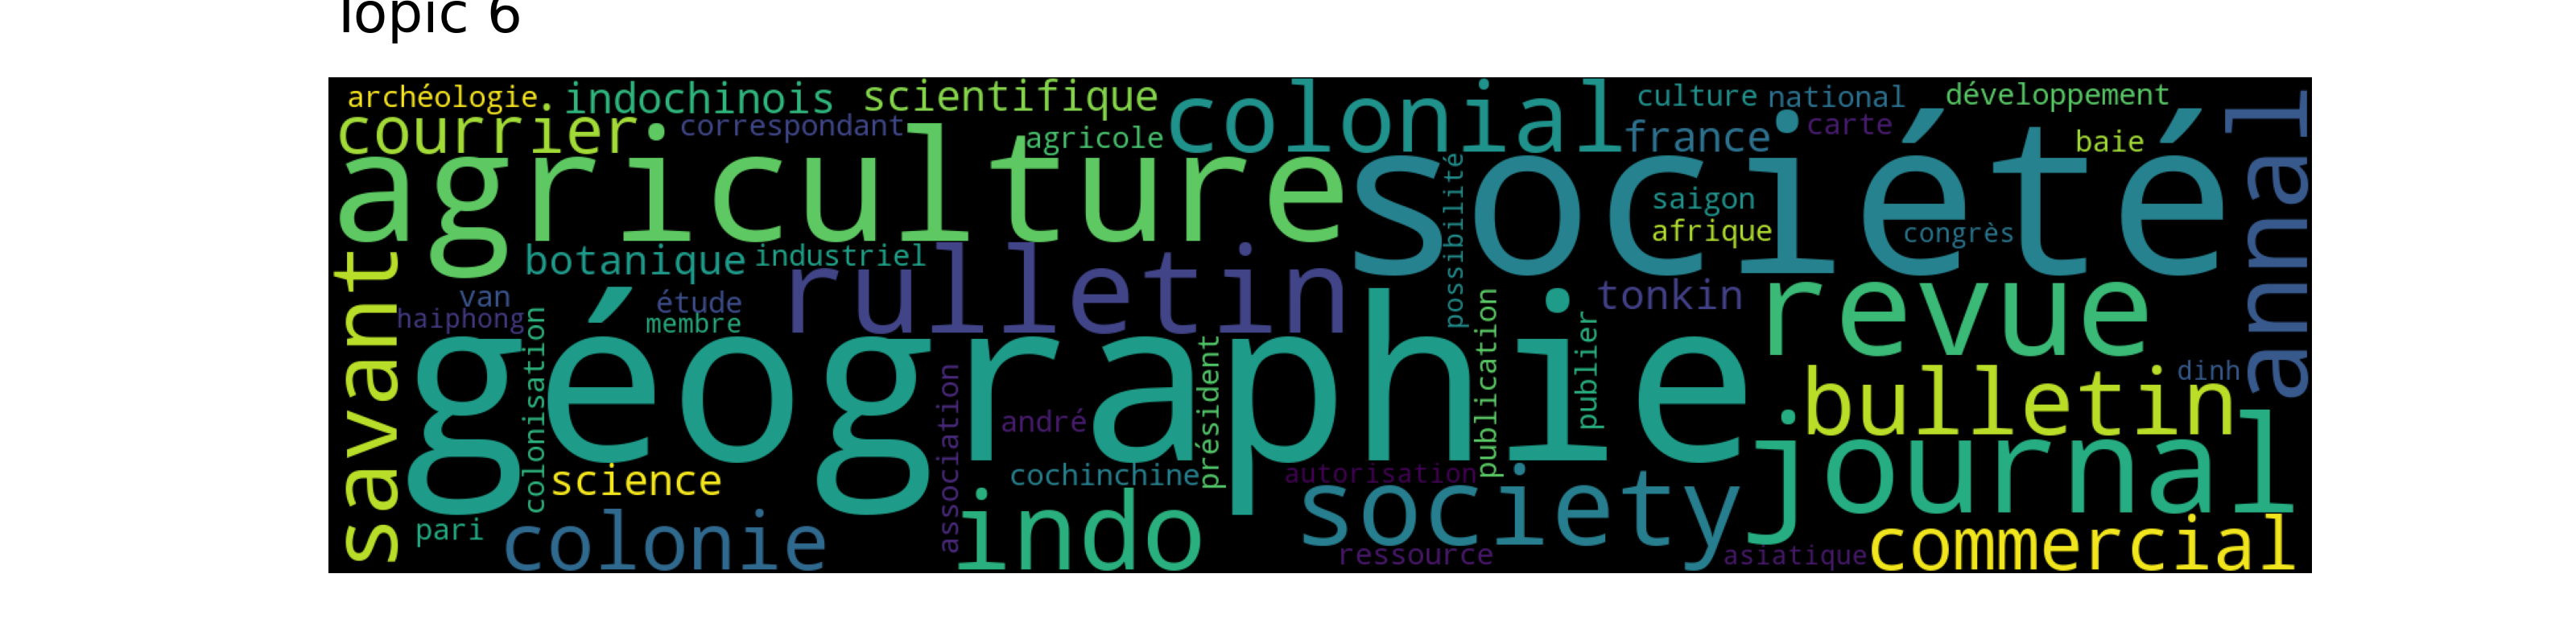
\includegraphics[width=14cm]{img/final_6_topic 6 .png}
    \caption{WordCloud du sujet }
    \label{tp6}
\end{figure}

Le modèle regroupe non seulement les sujets de mots-clés proches les uns des autres, mais distingue également implicitement les types de texte. Dans ce thème, l'agriculture, qui est le thème le plus important du corpus, revient, mais sous une forme différente. Il contient principalement des textes courts, de correspondances et les noms de livres dans la catégorie bibliographie ou publication, tous liés à l'agriculture et à la géographie.

En regardant la distribution des nombres sur la Figure \ref{fig:repartition_7topics}, on constate que c'est le sujet avec le moins de mots, mais cela est principalement dû au fait que les mots ont le même vocabulaire et les mêmes caractéristiques de longueur, ce qui les regroupe. Cela montre également qu'un modèle Top2vec avec une haute fréquence de mots n'atteint toujours pas des résultats optimaux pour les sujets.

Il est intéressant de constater que la répartition des articles et des mots dans les différents sujets varie considérablement. Certaines catégories, telles que l'agriculture et la plantation, les correspondants, et les activités de la société, contiennent de nombreux articles mais ces articles sont généralement courts en longueur. En revanche, d'autres sujets, tels que le militaire (à l'exception d'un biais lié aux textes des trois royaumes) et surtout la vie et la religion, peuvent avoir moins d'articles, mais ces articles sont souvent beaucoup plus longs.

Cette variation suggère qu'il existe un potentiel pour explorer davantage les sujets qui ont été moins développés dans le corpus. Par exemple, les sujets liés à la vie et à la religion pourraient offrir des opportunités de recherche approfondie, étant donné la longueur des articles disponibles dans ces catégories. Il est également possible qu'il existe de nombreux petits sujets inexplorés au sein de ces thèmes plus larges, ce qui pourrait permettre de découvrir de nouvelles perspectives et de nouvelles idées de recherche.

En fin de compte, l'analyse de la répartition des articles et des mots dans les différents sujets peut aider à identifier les domaines de recherche qui ont été moins explorés et à orienter les futurs travaux de recherche dans ces domaines. Cela peut contribuer à une compréhension plus complète des sujets abordés dans le B.S.E.I et à l'exploration de nouvelles pistes de recherche.

L'analyse du graphique révèle une certaine logique dans la proximité et la distance entre les thèmes abordés dans le B.S.E.I. Plusieurs observations peuvent être faites à partir de la visualisation sur la Figure \ref{umap7}.

\begin{figure}[H] %[!ht]
    \centering
    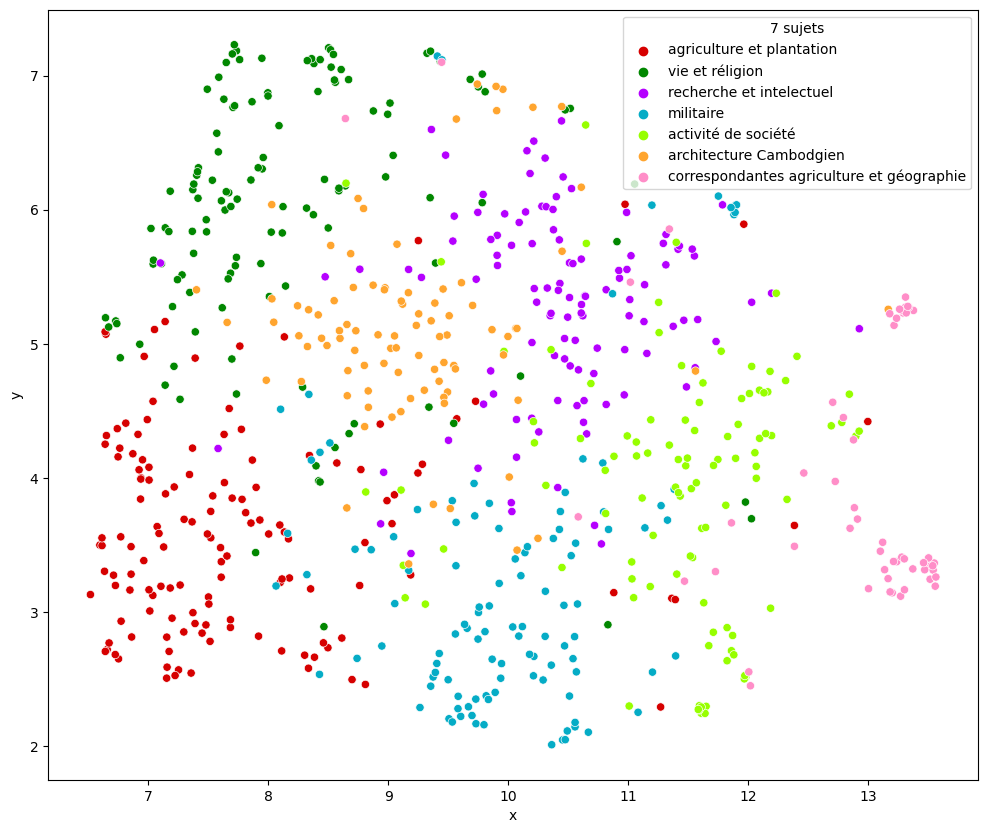
\includegraphics[width=14cm]{img/umap7.png}
    \caption{Projection spatial UMAP des vecteurs documents}
    \label{umap7}
\end{figure}

Proximité des thèmes : On remarque que les thèmes des activités de la société et les correspondants de l'association sont très proches les uns des autres dans le graphique. Cela suggère une certaine similarité ou corrélation entre ces deux catégories de sujets, ce qui est logique puisque les correspondants font partie intégrante des activités de la société.

Séparation des correspondants : Les correspondants de l'association sont complètement séparés des autres thèmes dans le graphique, ce qui indique qu'ils constituent une catégorie distincte et isolée. Cela reflète leur rôle particulier au sein de la société savante.

Proximité des thèmes de la vie et de la religion : Le thème de la vie et de la religion apparaît proche des thèmes de la vie de l'agriculture et des plantations, ainsi que du contenu de l'architecture religieuse du Cambodge. Cela suggère une connexion entre ces sujets, peut-être liée à l'influence de la religion sur la vie quotidienne et l'agriculture dans la région.

Liens des sujets intellectuels : Les sujets intellectuels sont étroitement liés à la société et à la plupart des autres thèmes dans le graphique. Cela suggère que l'intellectualisme était un élément central dans les activités de la société savante et qu'il était souvent en relation avec d'autres domaines de recherche.

En résumé, le graphique met en lumière les relations et les connexions entre les thèmes abordés dans le B.S.E.I. Il offre des informations précieuses sur la manière dont ces sujets étaient organisés et liés au sein de la société savante, ce qui peut aider à mieux comprendre la structure et l'orientation de la recherche menée par la Société des Études Indochinoises.

\subsubsection{Discussion}
En éliminant préalablement les documents moins pertinents par rapport à notre objectif de recherche, nous avons réussi à construire un modèle Top2Vec plus compact et équilibré en termes de nombre de documents, ainsi qu'à regrouper des documents similaires en termes de sens et de caractéristiques. 

Cependant, il est clair que cette approche n'a pas suffisamment contribué à extraire des sous-thèmes plus spécifiques. En effet, dans le modèle actuel composé de 7 thèmes, les thèmes principaux restent relativement redondants par rapport au modèle précédent qui en comportait 12. Il semble donc que cette méthode de filtrage ne soit pas aussi efficace que souhaité. Pour aller plus en profondeur dans l'exploration du corpus et découvrir des sujets plus détaillés, notamment en termes de vocabulaire, nous envisageons d'utiliser Word2Vec, dont nous présenterons l'application dans la section suivante.
\newpage 
\subsection{Avec l'application de Word2Vec}
\subsubsection{Introduction}
La technique du \textbf{Word Embedding} est un pilier fondamental du Traitement Automatique du Langage Naturel (NLP) qui transforme des mots ou des phrases en vecteurs numériques dans un espace de grande dimension continue. L'idée essentielle consiste à représenter les mots de manière à capturer leurs relations sémantiques et syntaxiques. Cette représentation permet aux modèles d'apprentissage automatique de mieux appréhender et exploiter les données textuelles, car elle encode des informations sur la signification des mots, les contextes et les similitudes.

En règle générale, les Word Embeddings sont appris à partir de vastes corpus de textes grâce à des techniques non supervisées. En plaçant les mots ayant des significations ou des utilisations similaires à proximité les uns des autres dans l'espace d'intégration, ces modèles d'intégration de mots contribuent à saisir la structure sémantique du langage. Parmi les modèles d'intégration de mots populaires, citons Word2Vec, GloVe (Global Vectors for Word Representation), et FastText.

Word2Vec représente un modèle d'intégration de mots spécifique, introduit par Tomas Mikolov et son équipe de Google en 2013 \footcite{DBLP:journals/corr/MikolovSCCD13}, marquant ainsi le début d'une ère nouvelle dans le domaine du NLP.

Word2Vec est un algorithme d'apprentissage automatique qui permet de créer des représentations vectorielles de mots, appelées embeddings. Ces embeddings sont utilisés dans diverses tâches de traitement du langage naturel, notamment le regroupement de mots, la classification et la génération de texte \footcite{articleMikolovW2V}. Pour ce faire, Word2Vec exploite des réseaux de neurones pour apprendre ces embeddings à partir de vastes quantités de données textuelles. Les résultats sont des vecteurs, un par mot du corpus d'apprentissage, qui capturent efficacement les relations entre les mots.

Dans l'espace vectoriel ainsi créé, des vecteurs proches les uns des autres signifient que les mots ont des sens similaires en fonction du contexte, tandis que des vecteurs éloignés indiquent des sens différents. Par exemple, les mots "Hanoï" et "Saigon" seraient proches, tandis que "Saigon" et "véhicule" seraient plus éloignés. Cette caractéristique représente une amélioration significative par rapport au modèle "sac de mots" qui se contente de compter les occurrences de mots dans un corpus de données textuelles. \footcite{inproceedingsWord2vec}.

Les modèles Word2Vec sont remarquablement efficaces sur le plan informatique, capables de gérer de vastes vocabulaires et corpus textuels. Les embeddings résultants sont utiles dans de nombreuses applications de NLP, comme l'analyse des sentiments, la traduction automatique, les systèmes de recommandation et le regroupement de documents. Ils permettent aux machines de comprendre et de travailler avec des données textuelles en reflétant la sémantique sous-jacente du langage, faisant ainsi office de pierre angulaire des applications modernes de NLP.

\subsubsection{Entraînement du modele Word2Vec}
Dans cette étude, nous allons explorer Gensim, une bibliothèque Python très répandue pour la création de modèles d'apprentissage automatique basés sur du texte. Nous allons l'utiliser pour former un modèle Word2Vec. Un modèle Word2Vec est créé en appelant la fonction suivante :

\begin{lstlisting}
from gensim.models import Word2Vec
from nltk.tokenize import word_tokenize

# Create and train a Word2Vec model
model_w2v = Word2Vec(sentences=tokenized_corpus, vector_size=1000, window=10, min_count=20, sg=0)

# Get the word vector for a specific word
word_vector = model_w2v.wv['scienctifique']

# Find similar words to a given word
similar_words = model_w2v.wv.most_similar('science', topn=20)

\end{lstlisting}

\textbf{vector\_size} spécifie la dimensionnalité des vecteurs de mots (incorporations de mots) que le modèle Word2Vec apprendra. vector\_size = 100 par exemple détermine la longueur des vecteurs représentant chaque mot dans l'espace d'intégration. Des vecteurs de plus grande taille peuvent capturer des relations plus complexes entre les mots, mais nécessitent plus de données d'entraînement et de mémoire.

\textbf{window} définit la distance maximale entre le mot actuel et le mot prédit dans une phrase (ou un contexte).
Il contrôle la taille de la fenêtre contextuelle du modèle.
Par exemple, si \textit{window = 5}, le modèle prend en compte les cinq mots avant et les cinq mots après le mot actuel lors de l'apprentissage des incorporations de mots.
Une taille de fenêtre plus petite capture les relations locales entre les mots, tandis qu'une taille de fenêtre plus grande capture un contexte plus global.

\textbf{min\_count }spécifie le nombre minimum (fréquence) d'un mot dans le corpus pour qu'il soit pris en compte lors de la formation ce qui est similaire à son utilisation dans Top2Vec.

La visualisation des intégrations Word2Vec à l'aide de t-SNE (t-Distributed Stochastic Neighbor Embedding) peut être un outil précieux pour observer la manière dont les mots se regroupent dans un espace de dimension réduite.

Dans un graphique de visualisation t-SNE, les deux axes représentent un espace bidimensionnel dans lequel les données de grande dimension (dans ce cas, les embeddings de mots Word2Vec) sont projetées. En d'autres termes, l'algorithme t-SNE tente de disposer les points de données (dans ce contexte, les mots) de manière à ce que les mots similaires soient proches les uns des autres et que les mots différents soient éloignés les uns des autres dans cet espace bidimensionnel.

La Figure \ref{sne} présente une telle distribution pour les mots qui apparaissent au moins 100 fois dans le corpus. On peut facilement remarquer que les mots regroupés sont très similaires, par exemple : (roi, empereur, titre, troupe), (mer, terre, eau), (Van, Thi, Nguyen, Vietnamien), (homme, femme), (famille, père, vie, mort), (séance, président, comité, membre), etc.

Cette représentation visuelle permet de mettre en évidence les relations sémantiques et syntaxiques entre les mots, facilitant ainsi la compréhension des regroupements de mots ayant des significations similaires dans l'espace Word2Vec.

\begin{figure}[H] %[!ht]
    \centering
    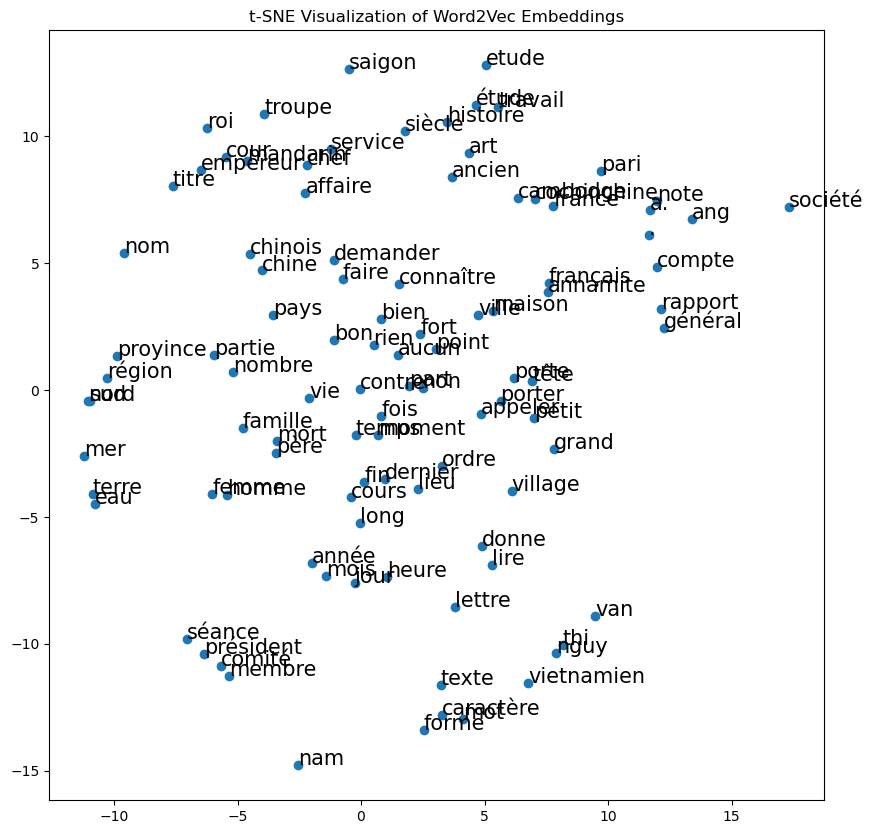
\includegraphics[width=14cm]{img/SNE.png}
    \caption{Distribution stochastique des voisins t-SNE}
    \label{sne}
\end{figure}

\subsubsection{Application des vecteurs Word2Vec pour la recherche des sujets}

Dans cette section, nous allons utiliser Word2Vec pour extraire un ensemble de mots-clés liés à notre thème d'intérêt, qui est la recherche et la science. Nous allons commencer par fournir une liste de mots-clés classiques associés à la science. Un modèle Word2Vec déjà entraîné sera capable de calculer et de retourner une liste de mots de longueur arbitraire considérés comme "similaires" dans leur espace vectoriel.

En étudiant cette liste, nous pourrons sélectionner différents mots ou collocations de mots qui pourraient représenter différents axes de recherche que nous souhaitons découvrir dans les couches internes de chaque sujet donné par Top2Vec. Nous aurons également la possibilité d'étendre cette liste en prenant chaque mot de la liste initiale et en demandant à Word2Vec de trouver de nouveaux mots similaires.

Cette approche nous permettra d'explorer et d'identifier des concepts et des domaines spécifiques liés à la recherche et à la science, en utilisant les informations capturées dans l'espace sémantique des mots par le modèle Word2Vec.

\textbf{Recherche des mots similaires}

En réalité, Top2Vec propose également une fonction pour rechercher des mots similaires en se basant sur ce qu'il a appris lors de la modélisation des sujets. Cependant, d'un point de vue algorithmique, l'objectif principal de Top2Vec n'est pas la similarité des mots. Il découvre des sujets dans un corpus et associe des mots à ces sujets. Bien que nous puissions mesurer la similarité entre des sujets ou des documents avec Top2Vec, il n'est pas principalement conçu pour les tâches de similarité entre les mots.

En revanche, Word2Vec apprend des représentations continues des mots dans un espace vectoriel de telle manière que des mots similaires soient regroupés à proximité les uns des autres dans cet espace vectoriel.

Voici un exemple qui illustre comment la méthode `Word2Vec.similar\_to\_keyword()` fonctionne pour obtenir une liste de 20 mots similaires au terme "scientifique".
\begin{lstlisting}
model_W2V.wv.similar_by_word('science',20)
>>
[('scientifique', 0.8899936676025391),
 ('médecine', 0.887998640537262),
 ('international', 0.885227620601654),
 ('contribution', 0.8683810830116272),
 ('archéologie', 0.8623462319374084),
 ('ethnologie', 0.8555389046669006),
 ('collaboration', 0.849744439125061),
 ('universel', 0.8497161865234375),
 ('médical', 0.8341251611709595),
 ('orientaliste', 0.8278639316558838),
 ('enrichir', 0.8277556896209717),
 ('unesco', 0.8257268071174622),
 ('ethnographie', 0.8231016993522644),
 ('manuel', 0.8221821188926697),
 ('revue', 0.822064995765686),
 ('indochine', 0.8218351602554321),
 ('national', 0.8206552267074585),
 ('savant', 0.8202723264694214),
 ('philosophie', 0.8200579285621643),
 ('orientalisme', 0.8192302584648132)]
\end{lstlisting}

Nous pouvons effectuer une comparaison entre cette liste et ce que le modèle Top2Vec suggère, en tenant compte du fait que ces deux modèles ont été tous deux entraînés en utilisant la même fréquence d'occurrence minimale (min\_count = 10) afin de garantir la comparabilité des résultats.

\begin{lstlisting}
model_T2V.similar_words(['science'],20)
>>
    [('scientifique', 0.6902187722544227), ('philosophie', 0.5809475431503167), ('étude', 0.5521098714814373), ('université', 0.5203653772090963), ('asie', 0.5196150235942933), ('recherche', 0.5191305586368542), ('congres', 0.5051189088436547), ('histoire', 0.49536285900614574), ('orient', 0.4939587142138291), ('savant', 0.4929562825259586), ('institut', 0.49073761852770154), ('technique', 0.4883345871370738), ('connaissance', 0.4840244353445985), ('extrême', 0.4768467212086376), ('probleme', 0.4734519460738481), ('orientalisme', 0.47328741068810387), ('international', 0.470452656842586), ('humain', 0.46990407416850477), ('géographie', 0.4688430974692131), ('mathématique', 0.46787602909710624)]
\end{lstlisting}
Nous observons une différence entre les deux listes en ce qui concerne l'évaluation de la similarité entre les mots. Alors que le mot 'scientifique' reste en tête de liste car il est directement dérivé du mot 'science', les scores attribués par les deux modèles sont nettement différents : 0,8899 pour Word2Vec, mais seulement 0,6902 pour Top2Vec. Nous observons le même phénomène pour quelques autres mots, tels que 'savant' et 'orientalisme'.

Cela peut s'expliquer par l'objectif de l'entraînement de chaque modèle : Word2Vec est formé pour prédire les mots contextuels à partir d'un mot cible (modèle Skip-gram) ou vice versa (modèle Continuous Bag of Words). Cet objectif conduit à la création de vecteurs de mots où des mots sémantiquement similaires sont regroupés étroitement dans l'espace vectoriel.

En revanche, Top2Vec est conçu pour découvrir des sujets puis associer des mots à ces sujets. Son objectif principal est de regrouper les mots dans des sujets plutôt que de créer des embeddings de mots basés sur la similarité sémantique.

En ce qui concerne la richesse et la variété du vocabulaire, Word2Vec présente un avantage avec une plus grande diversité de mots spécifiques couvrant différents domaines scientifiques. Sur une liste de 50 mots similaires, nous nous intéressons particulièrement aux mots qui désignent des domaines scientifiques tels que : médecine, archéologie, orientalisme, ethnographie, philosophie, géographie, anthropologie, sociologie, astrobiologie, anatomie, et paléontologie.

En revanche, avec Top2Vec, la sélection de mots liés aux domaines scientifiques est un peu plus restreinte : histoire, orientalisme, géographie, mathématiques, astronomie, linguistique, physique, archéologie, et anthropologie.

Il est effectivement notable que Word2Vec offre une plus grande variété de termes. Cette différence peut s'expliquer en partie par la dimensionnalité des embeddings de mots, qui est plus élevée dans Word2Vec et permet ainsi de capturer des relations sémantiques plus nuancées.

En plus de trouver des mots liés aux disciplines scientifiques, Word2Vec est également capable d'identifier des entités de personnes qui ont travaillé dans la recherche à l'époque, telles que Renou, Burnouf, Herbert, Grosset, et Fistoir. En revanche, Top2Vec ne propose aucune entité de ce type dans sa liste. Cette capacité de Word2Vec à extraire des entités spécifiques est un exemple de sa capacité à capturer des informations sémantiques fines et des relations contextuelles entre les mots. Il peut être particulièrement utile pour identifier des chercheurs, des auteurs ou d'autres entités spécifiques dans un corpus de texte. Cela met en évidence l'avantage de Word2Vec dans la découverte de termes spécifiques et d'entités dans le domaine de la recherche scientifique.

\textbf{Exploration de sujets à partir de mots-clés}

Après avoir obtenu la liste de mots-clés similaires à notre mot-cible, comme par exemple 'science', nous avons la possibilité d'utiliser une méthode de l'API du modèle Top2Vec pour découvrir les documents les plus pertinents dans divers domaines scientifiques.

Illustrons cela avec le terme 'médecine'. Nous trouvons ci-dessous un extrait de code permettant d'extraire les documents liés à un mot-clé donné. L'argument num\_doc=10 indiquera de récupérer les 10 documents les mieux classés en termes de similarité :

\begin{lstlisting}
from top2vec import Top2Vec

num_doc = 10
keyword = 'médecine'
model = Top2Vec.load('model_ngram_10_deep-learn')

[search_doc,search_score, search_doc_ID] = model.search_documents_by_keywords([keyword],num_doc)
for id,score in zip(search_doc_ID, search_score):
    print(score, ";" ,id, ";" ,data[id]["FolderName"])
\end{lstlisting}

Et voici le résultat :
\begin{lstlisting}
0.6868148446083069 ; 434 ; lãn-ông-et-la-médecine-sino-vietnamienne_1953_tome_xxviii
0.5724442601203918 ; 41 ; bio-bibliographie-de-la-médecine-chinoise_1956_tome_xxxi
0.46906882524490356 ; 318 ; bibliographie-etudes-historiques-sur-l-ancienne-médecine-au-viêt-nam-et-en-chine_1955_tome_xxx
0.44850513339042664 ; 95 ; histoire-de-l-acupuncture-chinoise_1959_tome_xxxiv
0.3707107901573181 ; 357 ; de-la-diffusion-de-la-médecine-européenne-en-cochinchine_1895_3e-fascicule
0.3464908003807068 ; 472 ; quelques-aspects-de-la-pénétration-des-sciences-occidentales-au-japon-depuis-le-xvie-siècle_1952_tome_xxvii
0.33641865849494934 ; 573 ; la-science-au-viêt-nam_1963_tome_xxxviii
0.3148581087589264 ; 206 ; panorama-médical-du-viêt-nam-d-autrefois_1951_tome_xxvi
0.23182639479637146 ; 277 ; médecine-populaire-au-cambodge_1965_tome_xl
0.23011955618858337 ; 694 ; variétés_1959_tome_xxxiv_4
\end{lstlisting}

Parmi les 10 documents mentionnés, nous avons immédiatement identifié 7 documents liés à la médecine ou à des sujets médicaux. En examinant de plus près les trois documents restants avec les indices 472, 573 et 694, nous avons constaté une fréquence élevée de termes médicaux tels que 'médecine', 'médical', 'chirurgie', 'chirurgien', 'chirurgical', etc., comme le montre la figure \ref{fig:medical}, ce qui confirme la pertinence de la sélection effectuée par Top2Vec.

\begin{figure}[H] %[!ht]
    \centering
    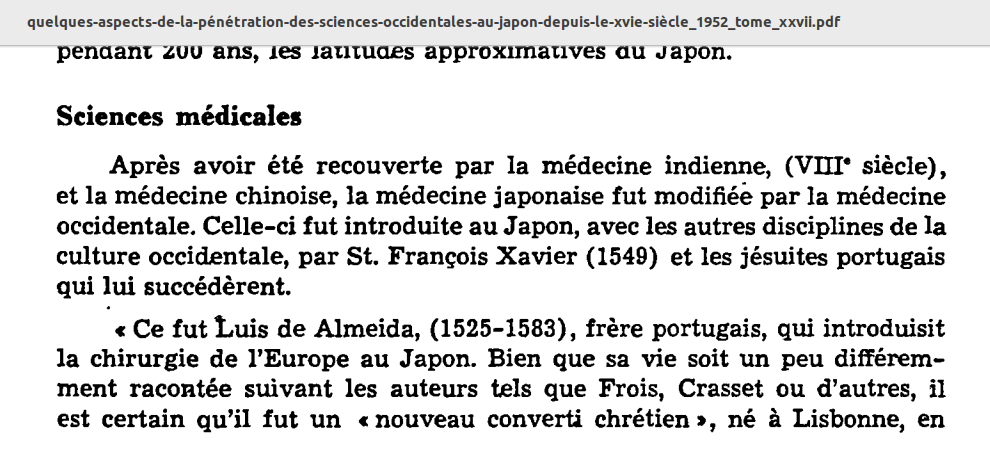
\includegraphics[width=14cm]{img/preuve_medecine_Top2Vec.png}
    \caption{Les textes medicaux dans l'article ID 472}
    \label{fig:medical}
\end{figure}

Un autre exemple qui illustre la performance de cette méthode concerne le terme 'laotien'. Comme mentionné précédemment, ce sujet spécifique se rapporte principalement aux ethnies laotiennes, mais il peut parfois être masqué sous des sujets plus généraux de recherche humaine. En utilisant cette technique, nous pouvons efficacement retrouver les documents relatifs à ce sujet plus spécifique parmi le corpus, même s'ils sont étroitement liés au sujet de recherche plus large.

\begin{lstlisting}
les-villages-du-plateau-des-bolovens_1951_tome_xxvi
le-dialecte-des-kha-boloven_1949_tome_xxiv
les-tribus-sek-et-kha-de-la-province-de-cammon_1950_tome_xxv
les-tribus-sô-de-la-province-de-cammon_1950_tome_xxv
rapport-à-m-le-gouverneur-général-par-j-taupin-résultat-de-sa-mission-au-laos_1888_semestre_2
monographie-de-la-province-de-stung-treng-cambodge_1913_semestre_1
monographie-de-la-province-de-savannakhet_1904_semestre_1
la-population-du-laos-en-1943-dans-son-milieu-géographique_1957_tome_xxxii
notes-sur-les-phou-theng-et-thai-bo_1949_tome_xxiv
essai-d-histoire-des-populations-montagnardes-du-sud-indochinois-jusqu-à-1945_1955_tome_xxx
\end{lstlisting}

C'est ainsi qu'en répétant cette méthode pour tous les mots-clés qui nous intéressent, les documents seront triés correctement avec un taux de réussite très élevé. Les termes sélectionnés et les résultats des documents pour ces termes sont présentés dans l'Annexe.

\textbf{**Exploration de documents dans diverses disciplines scientifiques**}

En examinant les mots suggérés par Word2Vec, nous avons finalement identifié les termes suivants qui représentent les disciplines de recherche à l'époque indochinoise : \textbf{\textit{ethnologie, philologie, sociologie, archéologie, géographie, ethnographie, anthropologie, médecine, orientalisme, philosophie, anatomie, paléontologie, économie, linguistique, précolombien, astrobiologie, philologue, préhistoire, astronomie, sinologie, mathématiques, et nationalisme}}. 

Pour garantir un certain niveau de précision dans les documents recherchés, nous avons appliqué un filtre aux résultats, exigeant que le score de similarité soit supérieur à 0,25. Il est important de noter que la méthode de notation de Top2Vec est assez exigeante, et avec un score d'environ 0,4, nous avons déjà pu identifier des documents étroitement liés à notre mot-clé. Les documents les plus pertinents dans chaque domaine de recherche, accompagnés de leurs scores et de l'année de publication, sont répertoriés dans l'annexe de ce mémoire.

Les figures \ref{fig:circle_topic} et \ref{fig:theme_nbdoc_scientifique} présentent la répartition des documents appartenant à différentes disciplines scientifiques que nous avons sélectionnées parmi les mots-clés les plus marquants. Parmi les sujets les plus populaires de l'époque, nous pouvons mentionner l'archéologie, la géographie, l'ethnologie, la préhistoire, la linguistique et la philosophie, qui englobent de nombreuses sciences humaines.

Malgré une limite en termes de quantité de documents disponibles, des domaines de recherche plus spécifiques et avancés tels que l'astronomie, la paléontologie et l'astrobiologie sont déjà présents dans ce corpus. Ils auraient tout à fait pu jouer un rôle pionnier dans la recherche dans ces domaines en Indochine.

\begin{figure} [H]%[!ht]
    \centering
    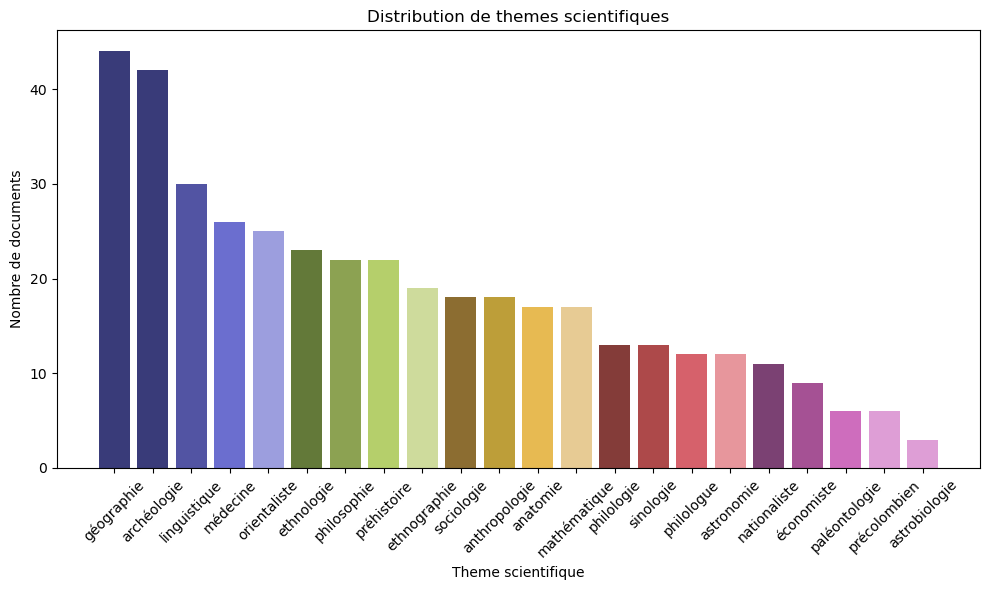
\includegraphics[width=14cm]{img/theme_nbdoc_scientifique_0.2.png}
    \caption{Nombre de documents par sujet scientifique}
    \label{fig:theme_nbdoc_scientifique}
\end{figure}

% "Nous examinerons successivement l'intérêt que présentent pour nos études: 1) l'histoire de la civilisation; 2) I ‘histoire de la technologie; 3) l'histoire des religions; 4) l'histoire des beaux-arts, enfin 5) les recherches archéologiques, anthropologiques et ethnologiques."\footnote{\cite{sarton}}


\begin{figure} [t]%[!ht]
    \centering
    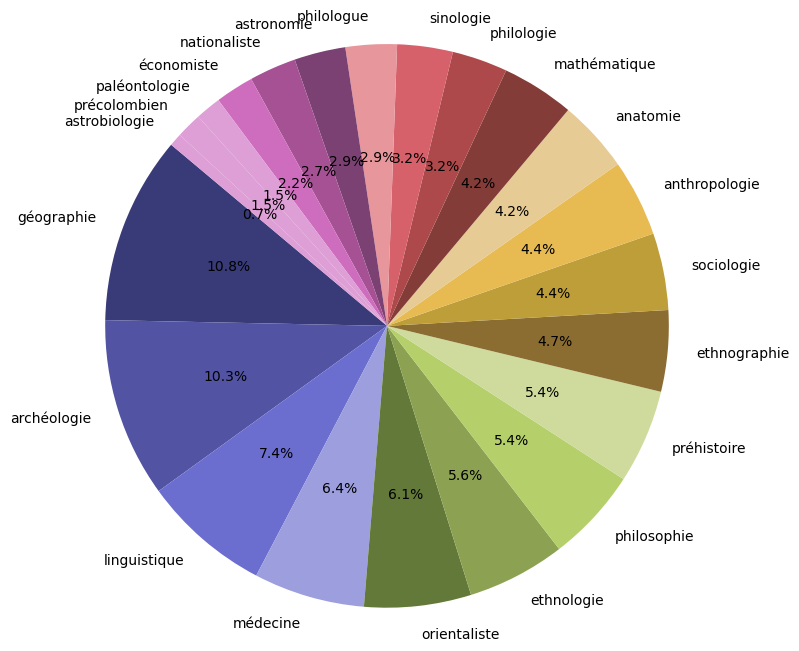
\includegraphics[width=14cm]{img/circle_topic.png}
    \caption{ Partitions des disciplines scientifiques}
    \label{fig:circle_topic}
\end{figure}

% \begin{figure} [H]%[!ht]
%     \centering
%     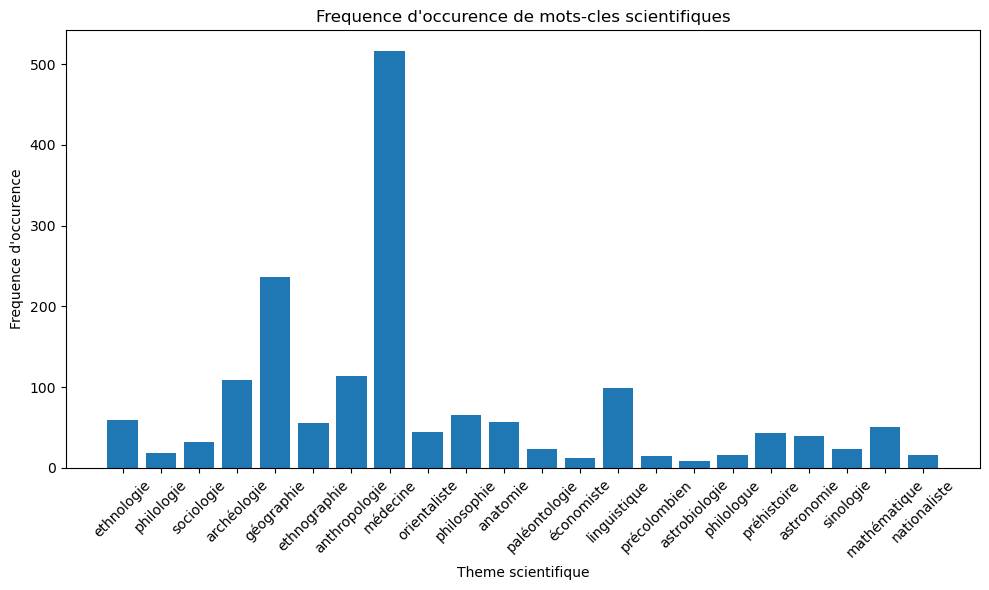
\includegraphics[width=14cm]{img/theme_freq_scientifique.png}
%     \caption{Frequence de mots-cles par sujet scientifique}
%     \label{fig:theme_freq_scientifique}
% \end{figure}

Dans la Figure \ref{fig:theme_freq_per_doc}, nous calculons la fréquence moyenne de présence du mot-clé par document. Malgré le fait que les documents médicaux ne représentent que le troisième plus grand nombre de documents, leur fréquence d'occurrence est exceptionnellement élevée par rapport aux autres termes. Cette observation souligne l'importance et la prévalence des sujets médicaux dans le corpus étudié.

\begin{figure} [H]%[!ht]
    \centering
    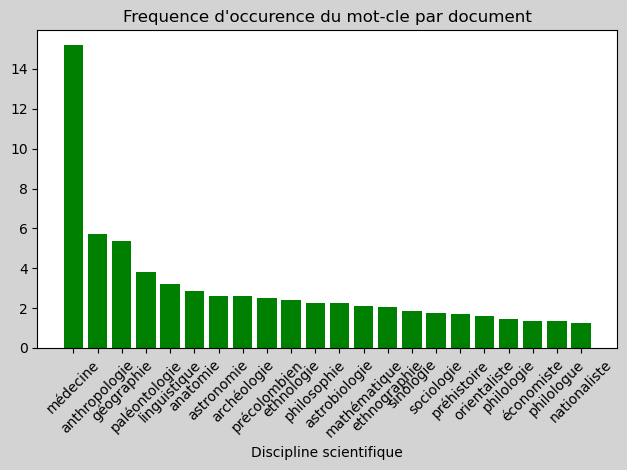
\includegraphics[width=14cm]{img/theme_freq_per_doc.png}
    \caption{Fréquence de mots-cléés par documents dans chaque sujet}
    \label{fig:theme_freq_per_doc}
\end{figure}

La figure \ref{fig:all_theme_year_scientifique} présente la distribution temporelle de toutes les disciplines scientifiques. En général, on observe une augmentation de la fréquence des documents scientifiques au fil du temps. Cependant, il est intéressant de noter que quatre années en particulier se démarquent par un nombre significativement plus élevé de documents, à savoir 1933, 1951, 1959 et 1971. Ces années pourraient avoir été marquées par des développements importants ou des événements particuliers qui ont conduit à une production accrue de documents scientifiques dans le domaine de l'Indochine. Une analyse plus approfondie des documents de ces années pourrait fournir des informations précieuses sur les tendances et les événements scientifiques de l'époque.

\begin{figure}[H] %[!ht]
    \centering
    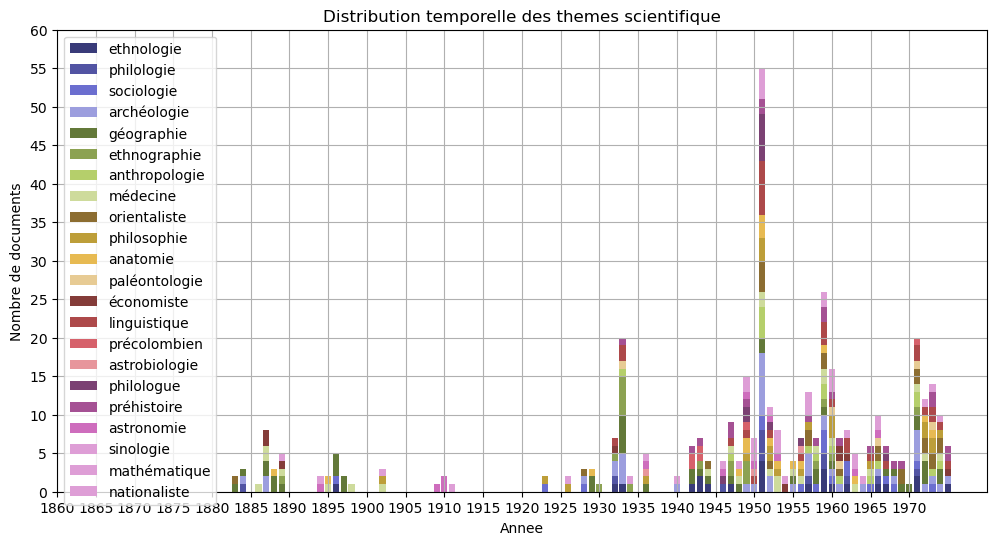
\includegraphics[width=14cm]{img/all_theme_year_scientifique.png}
    \caption{ Distribution de documents scientifique en periode Indochine}
    \label{fig:all_theme_year_scientifique}
\end{figure}

L'analyse des emplacements vides sur la carte thématique du B.S.E.I révèle des informations intéressantes sur l'évolution de la revue au fil du temps. Voici quelques observations à partir de cette analyse :

Évolution en deux étapes : Le graphique montre clairement deux étapes distinctes dans le développement du magazine. La première étape est caractérisée par un nombre limité de sujets fondamentaux, ce qui indique que la revue se concentrait principalement sur des domaines spécifiques de recherche. La seconde étape montre une diversification des sujets et une augmentation significative du nombre d'articles publiés chaque année.

Anniversaire du 50e anniversaire : En 1933, il y a une augmentation marquée du nombre de sujets et d'articles. Cela correspond au 50e anniversaire du lancement de la revue, ce qui suggère que cet événement a été célébré par une édition spéciale plus volumineuse et diversifiée.

L'année 1952 représente une exception notable dans l'histoire du B.S.E.I en raison du nombre exceptionnellement élevé de pages du journal publiées cette année-là, atteignant jusqu'à 602 pages. Cette situation se démarque nettement des normes générales observées dans l'ensemble du corpus de la revue.

Développement quantitatif et qualitatif : Au fil des ans, le nombre de sujets et d'articles dans la revue a continué de croître, indiquant un développement à la fois quantitatif et qualitatif. Cela suggère que la revue est devenue de plus en plus dynamique et productive au fil du temps.

En résumé, l'analyse des emplacements vides sur la carte thématique du B.S.E.I montre comment la revue a évolué au fil des ans, passant d'une phase de concentration sur des sujets spécifiques à une phase de diversification et de croissance. Cette évolution reflète la maturation et l'expansion de la société savante au fil du temps.

% \begin{figure}[H] %[!ht]
%     \centering
%     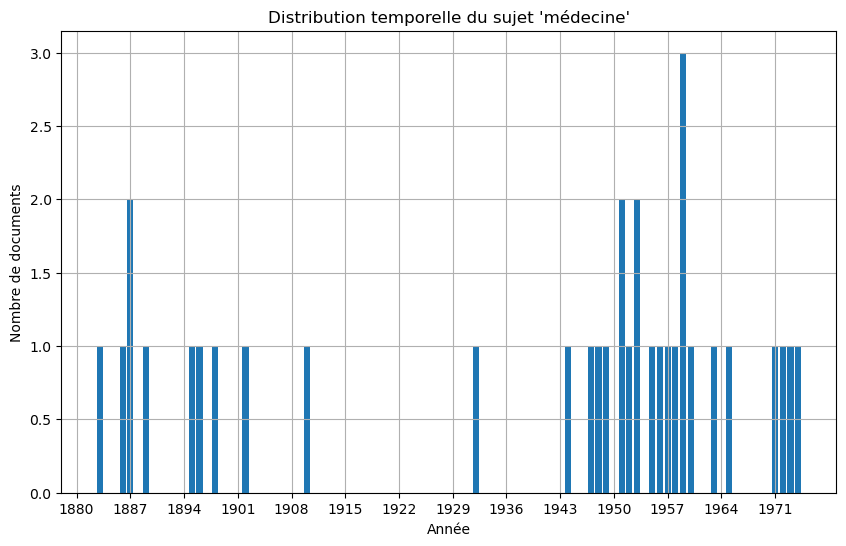
\includegraphics[width=14cm]{img/theme_year_medecine.png}
%     \caption{Distribution des document sujet medecine dans le temps}
%     \label{fig:theme_year_medecine}
% \end{figure}

\subsubsection{Discussion}
Dans cette section, l'utilisation de Word2Vec pour identifier des mots-clés importants s'est avérée extrêmement utile pour mettre en avant des sujets cachés au sein de diverses sources de documents, qui n'étaient pas encore suffisamment organisés par la méthode Top2Vec. Cette approche permet de résoudre le dilemme auquel Top2Vec est confronté lorsqu'il s'agit d'apprendre à partir de fréquences de mots trop faibles. En capitalisant sur la capacité du modèle Top2Vec à comprendre les termes à basse fréquence, nous pouvons désormais filtrer avec une grande précision les documents liés à des domaines de recherche spécifiques.

Cependant, il est important de noter que dans certains domaines où les recherches sont encore limitées à un stade précoce, il peut être difficile pour notre modèle de filtrer avec une précision absolue. Néanmoins, cette méthode permet au moins de repérer les documents qui mentionnent un domaine de recherche donné, ce qui peut ensuite faciliter la découverte d'autres documents importants, y compris ceux provenant d'autres agences correspondantes à travers le monde, et non seulement en Indochine.

